\documentclass[10pt,journal,compsoc]{IEEEtran}

% *** CITATION PACKAGES ***
%
\ifCLASSOPTIONcompsoc
  % IEEE Computer Society needs nocompress option
  % requires cite.sty v4.0 or later (November 2003)
  \usepackage[nocompress]{cite}
\else
  % normal IEEE
  \usepackage{cite}
\fi

\usepackage{booktabs} % For formal tables
\usepackage[utf8]{inputenc}
\usepackage[english]{babel}
\usepackage[T1]{fontenc}
\usepackage{url}
\usepackage{graphicx}
\usepackage{graphics}
\usepackage{listings}  
\usepackage{array}
\newcolumntype{L}[1]{>{\raggedright\let\newline\\\arraybackslash\hspace{0pt}}m{#1}}
\newcolumntype{C}[1]{>{\centering\let\newline\\\arraybackslash\hspace{0pt}}m{#1}}
\newcolumntype{R}[1]{>{\raggedleft\let\newline\\\arraybackslash\hspace{0pt}}m{#1}}
\usepackage{multirow}
%\usepackage[table]{xcolor}
\usepackage{float}
\usepackage{array}
\usepackage{ragged2e}
\usepackage{cleveref}
\usepackage{subcaption}
\usepackage{tikz}
\usepackage[normalem]{ulem}
\usepackage{amsmath}
\usepackage{amsfonts}

\newcolumntype{P}[1]{>{\RaggedRight\hspace{0pt}}p{#1}}

\lstset{language=Java,
	tabsize=2,
	basicstyle=\ttfamily\footnotesize,
	moredelim=[is][\dotuline]{@}{@},
	mathescape=true
} 

\newcommand{\squeezeup}{\vspace{-0.5mm}}

\usepackage{etoolbox}
\makeatletter
\patchcmd{\@makecaption}
{\scshape}
{}
{}
{}
\makeatother

\newcolumntype{"}{@{\hskip\tabcolsep\vrule width 1pt\hskip\tabcolsep}}

\newcommand\FIXME[1]{{\color{red}\textbf{FIXME: #1}}}

% correct bad hyphenation here
%\hyphenation{op-tical net-works semi-conduc-tor}

\begin{document}

\title{Outdated and License-Violating Code on Stack Overflow}

\author{Chaiyong Ragkhitwetsagul,~Matheus Paixao,~Jens Krinke,~Giuseppe Bianco,~Rocco Oliveto}

% The paper headers
\markboth{IEEE TRANSACTIONS ON SOFTWARE ENGINEERING,~Vol.~X, No.~Y, August~2017}%
{Ragkhitwetsagul \MakeLowercase{\textit{et al.}}: Outdated and License-Violating Code on Stack Overflow}
% The only time the second header will appear is for the odd numbered pages
% after the title page when using the twoside option.
% 
% *** Note that you probably will NOT want to include the author's ***
% *** name in the headers of peer review papers.                   ***
% You can use \ifCLASSOPTIONpeerreview for conditional compilation here if
% you desire.

% The publisher's ID mark at the bottom of the page is less important with
% Computer Society journal papers as those publications place the marks
% outside of the main text columns and, therefore, unlike regular IEEE
% journals, the available text space is not reduced by their presence.
% If you want to put a publisher's ID mark on the page you can do it like
% this:
%\IEEEpubid{0000--0000/00\$00.00~\copyright~2015 IEEE}
% or like this to get the Computer Society new two part style.
%\IEEEpubid{\makebox[\columnwidth]{\hfill 0000--0000/00/\$00.00~\copyright~2015 IEEE}%
%\hspace{\columnsep}\makebox[\columnwidth]{Published by the IEEE Computer Society\hfill}}
% Remember, if you use this you must call \IEEEpubidadjcol in the second
% column for its text to clear the IEEEpubid mark (Computer Society jorunal
% papers don't need this extra clearance.)

% for Computer Society papers, we must declare the abstract and index terms
% PRIOR to the title within the \IEEEtitleabstractindextext IEEEtran
% command as these need to go into the title area created by \maketitle.
% As a general rule, do not put math, special symbols or citations
% in the abstract or keywords.
\IEEEtitleabstractindextext{%
\begin{abstract}
% We studied online code clones on the popular programming Q\&A
% website, Stack Overflow, and their issues on outdated code and
% software licensing violations. 
\FIXME{Outdated.~Revise the last.}~Online code clones are code fragments that are copied from software
projects or online sources to Stack Overflow as examples in
questions and answers.
% They can be discovered by using code clone
% detectors, yet they are inherently different from normal code clones
% in software projects in several aspects. 
Due to an absence of a checking mechanism after the code has been
copied to Stack Overflow, online code clones may suffer from
becoming outdated or violating the original software license.
% Moreover, we also found that majority of online code clones do not
% contain the license of their originals.
We present a study incorporating several state-of-the-art tools and
techniques to automatically extract, prioritise, and filter detected
online clone pairs between 144,064 Java code snippets on Stack
Overflow and 111 Java open source projects in the curated Qualitas
corpus. We discovered and analysed 32,533 non-trivial online clone
candidates. Our investigation of 3,636 manually confirmed clone
pairs revealed strong evidence that 112 clones have been copied from
a Qualitas project to Stack Overflow.  We found 64 of them (57\%) 
to be outdated and potentially harmful for reuse.  Furthermore, we
found 357 code snippets on Stack Overflow that violate the license
of their original software.
% These snippets are questionable for reuse.
% Our study is among the first to address the problem of
% outdated and license-violating code snippets on Stack Overflow.
\end{abstract}

% Note that keywords are not normally used for peerreview papers.
\begin{IEEEkeywords}
Clone Detection, Stack Overflow, Outdated Code, Software Licensing
\end{IEEEkeywords}}


% make the title area
\maketitle


% To allow for easy dual compilation without having to reenter the
% abstract/keywords data, the \IEEEtitleabstractindextext text will
% not be used in maketitle, but will appear (i.e., to be "transported")
% here as \IEEEdisplaynontitleabstractindextext when the compsoc 
% or transmag modes are not selected <OR> if conference mode is selected 
% - because all conference papers position the abstract like regular
% papers do.
\IEEEdisplaynontitleabstractindextext
% \IEEEdisplaynontitleabstractindextext has no effect when using
% compsoc or transmag under a non-conference mode.



% For peer review papers, you can put extra information on the cover
% page as needed:
% \ifCLASSOPTIONpeerreview
% \begin{center} \bfseries EDICS Category: 3-BBND \end{center}
% \fi
%
% For peerreview papers, this IEEEtran command inserts a page break and
% creates the second title. It will be ignored for other modes.
\IEEEpeerreviewmaketitle

\IEEEraisesectionheading{\section{Introduction}\label{sec:introduction}}

%The popularity of the Internet encourages tremendous amount of source code being shared online. 
Stack Overflow is a popular online programming community with 7.6
million users, 14 million questions, and 23 million answers\footnote{Data as of 21
	August 2017 from~\url{https://stackexchange.com/sites}}. It allows programmers to ask questions and give answers
to programming problems. The website has found to be useful for
software
development~\cite{Ponzanelli2013,Ponzanelli2014,Keivanloo2014,Park2014,
	Stolee2014,Subramanian2013,Diamantopoulos2015,Treude2016} and also
valuable for educational purposes~\cite{Nasehi2012}. On Stack
Overflow, each conversation contains a question and a list of
answers. The answers frequently contain at least one code snippet as
a solution to the question asked. We found that the code snippets are
usually not authored directly on the Stack Overflow website but copied
from another location. A snippet in an answer could be copied and modified
from a code snippet in the question, copied from the answerer's own
code or from other locations including open source software (OSS)
systems. The process of posting and answering questions on Stack
Overflow that involves reusing of source code, can be considered as
code cloning.

Code cloning is an activity of reusing source code by copying and
pasting. It normally occurs in software development and account from
7\% to 23\% of source code in typical software
systems~\cite{Bellon2007}. The benefits and drawbacks of clones are
still controversial. Several authors state that clones lead to bug
propagations and software maintenance issues~\cite{Kamiya2002}, while
some others suggest that clones are not harmful and can even be
beneficial~\cite{Saini2016,Kapser2006}.

Code cloning can also have side effects such as violating software
licenses or introducing software vulnerabilities. Carelessly cloning
code from one project to another project with a different license may
cause a software licensing violation~\cite{German2009}. This also
happens within the context of online Q\&A websites such as Stack
Overflow. An et al.~\cite{An2017} showed that 1,279 cloned snippets
between Android apps and Stack Overflow potentially violate software
licenses. Security is also among the main concerns when code is copied
from an online source. For example, Stack Overflow helps developers to solve
Android programming problems more quickly than other resources while,
at the same time, offers less secure code than books or the official
Android documentation~\cite{Acar2016}.

We call code snippets that are copied from software systems to online
Q\&A websites (such as Stack Overflow) and vice versa as ``online
code clones''. There are two
directions in creating online code clones: (1) code is cloned from a software
project to a Q\&A website as an example; or (2) code is cloned from a
Q\&A website to a software project to obtain a functionality, perform
a particular task, or fixing a bug.
% and (3) code is transferred from one software project to another via a Q\&A website; 
Similar to classic clones, online code clones can lead to license
violations, bug propagation, introduction of vulnerabilities, and
re-use of outdated code. Unfortunately, online clones are 
difficult to locate and fix since the search space in online code
corpora is larger and no longer confined to a local repository.

The findings from our online survey of Stack Overflow answerers show that code
reusing activity occurs on Stack Overflow, just like in software. Stack Overflow
answerers occasionally clone code from other locations, such as their personal
projects, company projects, and open source projects, to Stack Overflow answers
as a solution or to complement their answer~\FIXME{put a precise number here}.
One participants says

\begin{quote}\textit{The real issue is less about the amount the code snippets
		on SO than it is about the staggeringly high number of software
		``professionals'' that mindlessly use them without understanding what they're
		copying, and the only slightly less high number of would-be professionals that
		post snippets with built-in security issues.  A related topic is beginners who
		post (at times dangerously) misleading tutorials online on topics they actually
		know very little about. Think PHP/MySQL tutorials written 10+ years after
		\texttt{mysql\_*} functions were obsolete, or the recent regex tutorial that
		got posted the other day on HackerNew
		(\url{https://news.ycombinator.com/item?id=14846506}). They're also full of
		toxic code snippets.}\end{quote}

With the same analogy, in this study we are interested in mining Stack Overflow
posts, detecting online code clones, and revealing \textbf{toxic code snippets},
which means code snippets that are harmful for reuse.
Stack Overflow snippets can become toxic because they are outdated and violating
their original software license. Outdated code snippets can be harmful since
they may contain defects. Moreover, licensed code snippets that are cloned from
open source software projects to Stack Overflow without their respective license
can lead to legal issues if being reused.

\begin{figure*}
	\begin{lstlisting}
/* Code in Stack Overflow post ID 22315734 */         /* WritableComparator.java (2017-10-03) */
public int compare(byte[] b1,int s1,int l1, ...) {    public int compare(byte[] b1,int s1,int l1, ...) {
  try {                                                 try {
    buffer.reset(b1,s1,l1); /* parse key1 */              buffer.reset(b1,s1,l1); /* parse key1 */
    key1.readFields(buffer);                              key1.readFields(buffer);
    buffer.reset(b2,s2,l2); /* parse key2 */              buffer.reset(b2,s2,l2); /* parse key2 */
    key2.readFields(buffer);                              key2.readFields(buffer);
  } catch (IOException e) {                               $$@buffer.reset(null,0,0); /* clean up reference */@
    throw new RuntimeException(e);                      } catch (IOException e) {
  }                                                       throw new RuntimeException(e);
  return compare(key1,key2); /* compare them */         }
}                                                       return compare(key1, key2); /* compare them */
                                                      }
	\end{lstlisting}\vspace{-2ex}
	\caption{A motivating example of the two code fragments of
		{\small\texttt{WritableComparator.java}}. The one from the
		Stack Overflow post 22315734 (left) is outdated when compared to
		its latest version in the \textsf{hadoop} code base
		(right).}
	\label{fig:before-after}
\end{figure*}

We would like to motivate the readers to the problem of toxic code snippets
on Stack Overflow by giving two examples.

The first motivating example of outdated online code clones can be found in an
answer to a Stack Overflow question regarding how to implement
{\small{\texttt{RawComparator}}} in
\textsf{hadoop}\footnote{\url{http://stackoverflow.com/questions/22315734}}.
\Cref{fig:before-after} shows---on the left---a code snippet embedded as a part
of the accepted answer. The snippet shows how \textsf{hadoop} implements the
{\small{\texttt{compare}}} method in its {\small{\texttt{WritableComparator}}}
class. The code snippet on the right shows another version of the same method,
but at this time extracted from the latest version (as of October 3, 2017) of
\textsf{hadoop}. We can see that they both are highly similar except a line
containing {\small{\verb|buffer.reset(null,0,0);|}} which was added on November
21, 2014. The added line is intended for cleaning up the reference in the
{\small{\verb|buffer|}} variable and avoid excess heap usage
(HADOOP-11323\footnote{https://issues.apache.org/jira/browse/HADOOP-11323}).
While this change has already been introduced into the
{\small{\texttt{compare}}} method for several years, the code example in Stack
Overflow post is still unchanged. 
%This example shows that inconsistencies
%between online code clones and their originals can lead users of Stack Overflow
%to reuse outdated code. 
In addition, although the original code snippet of
WritableComparator.java in Hadoop is subject to Apache license version 2.0, the
cloned code on Stack Overflow contains only a {\small{\texttt{compare}}}
method and misses its license statement on top of the file. There are two
potential issues for this. First, the code snippet may look like it is under
Stack Overflow's CC BY-SA 3.0 instead of its original Apache license. Second, if
the code snippet is copied and incorporated into another software project with
conflicting license, a legal issue may arise.

\begin{figure*}
	\begin{lstlisting}
/* Code in Stack Overflow post ID 801987 */             /* StringUtils.java (2017-10-03) */
public static String humanReadableInt(long number) {    public static String humanReadableInt(long number) {
  long absNumber = Math.abs(number);                      return TraditionalBinaryPrefix.long2String(number,"",1);
  double result = number;                               }
  String suffix = "";
  if (absNumber < 1024) {
  } else if (absNumber < 1024 * 1024) {
    result = number / 1024.0;
    suffix = "k";
  } else if (absNumber < 1024 * 1024 * 1024) {
    result = number / (1024.0 * 1024);
    suffix = "m";
  } else {
    result = number / (1024.0 * 1024 * 1024);
    suffix = "g";
  }
  return oneDecimal.format(result) + suffix;
}
	\end{lstlisting}\vspace{-2ex}
	\caption{A motivating example of the two code fragments of
		{\small\texttt{StringUtils.java}}. The one from the
		Stack Overflow post 801987 (left) is outdated when compared to
		its latest version in the \textsf{hadoop} code base
		(right). The outdated code has race conditions.}
	\label{fig:before-after_2}
\end{figure*}

The second motivating example of outdated online code clones with more
disrupting changes than the first one  can be found in an answer to a Stack
Overflow question regarding how to format files sizes in a human readable form.
\Cref{fig:before-after_2} shows---on the left---a code snippet to perform the
task from {\small{\texttt{StringUtils}}} class in \textsf{hadoop}. The code snippet on the
right shows another version of the same method, but at this time extracted from
the latest version of \textsf{hadoop}. We can see that
they both are totally different. The {\small{\texttt{humanReadableInt}}} method is
rewritten on February 5, 2013 to solve an issue of a race condition
(HADOOP-9252\footnote{https://issues.apache.org/jira/browse/HADOOP-9252}).

This two toxic code snippet has been posted on March 11, 2014 and April 9, 2009
respectively. They have already been viewed 259 and 2,886 times as the time of
writing this paper (October 3, 2017). Our calculation finds that there will be a
new viewer of the first toxic snippet in approximately every 5 days while the
second toxic snippet will be viewed almost every single day. Moreover, a
quick web search shows that the same {\small{\texttt{humanReadableInt}}}
method already reside in approximately 500 projects on GitHub. Considering the popularity of Stack
Overflow, which has more than 50 million developers visiting each
month\footnote{Data as of 21 August 2017 from: \url{https://stackoverflow.com}},
one toxic code snippets on Stack Overflow can spread and grow to hundred or
thousand copies within only a year or two.

%The code snippet on Stack Overflow can be outdated. %Since reusing source code from Stack Overflow is considered a common practice nowadays, the scale of online code cloning is more than intra or inter project clone in a local code bases.
%This is an emerging and challenging problem. Since studies in this area are still limited, we aim to gain more insight of the problem in this study. %We are interested to gain more insights of online code clone in this study.

While research has mostly focused on reusing code snippets \emph{from} Stack
Overflow (e.g.~\cite{Keivanloo2014,An2017,Yang2016}), fewer studies have been
conducted on finding the origins of code examples copied \emph{to} Stack
Overflow and the awareness of Stack Overflow developers in doing so. Finding the
origins of code examples gives insights to the problems of toxic code snippets
including outdated code and software licensing violations. It is probably more
important than studying the effects of reusing Stack Overflow code snippets
because it tackles the root cause of the problem. Moreover, this paper lays a
foundation to possibility of having an automatic technique to detect and report
such problems to developers in the future.

This paper fills this gap and makes the following primary contributions:

\begin{enumerate} 
	\item \textbf{A manual study of online code clones:} We used
	two clone detection tools to discover 315,786,118 similar code snippet pairs,
	followed by a manual classification of 3,636 candidate clone pairs between
	144,064 Java code snippets obtained from Stack Overflow's accepted answers and
	111 Java open source projects from the curated Qualitas
	corpus~\cite{QualitasCorpus}. 
	
	\item \textbf{An investigation of outdated and
		license-violating online clones on Stack Overflow:} Our study shows that from
	the 3,636 online clones, at least 671 likely have been copied from open source
	projects or external online sources to Stack Overflow, potentially violating
	software licenses. For 112 of them, we found evidence that they have been copied
	from a specific Qualitas project and that 64 of them are meanwhile outdated. %
	% and questionable for being reused.
	
	\item \textbf{Awareness of Stack Overflow answerers to
	toxic code snippets:} We performed an online survey and collected answers from
	202 highly-ranked Stack Overflow developers. We found that there are~\FIXME{add
	the number here}\% of code snippets cloned from open source projects to Stack
	Overflow answers. While Stack Overflow answerers are aware of their outdated
	code snippets, 19\% of the participants report that they rarely or never fix
	the code. At least 98\% of the answerers never include software license in
	their snippets and 69\% never check for licensing conflicts with Stack
	Overflow's CC BY-SA 3.0 if they copy the code from other sources to Stack
	Overflow answers.
	
	\item \textbf{An online code
		clone oracle:} The 2,302 manually investigated and validated online clone pairs
	are available for download\footnote{https://to.be.disclosed.after.review} and
	can be used as a clone oracle. \end{enumerate}

\section{Empirical Study}

We performed an empirical study of online code clones between Stack
Overflow and 111 Java open source projects to answer the following
research questions:
\begin{itemize}
	\item \textbf{RQ1 (Online code clones): }\textit{To what extent is source
		code cloned between Stack Overflow and open source projects?} We
	quantitatively measured the number of online code clones between Stack
	Overflow and open source projects to understand the scale of the
	problem. 
	\item \textbf{RQ2 (Patterns of online code clones): }\textit{Why do online
		code clones occur?} We categorised online clones into seven
	categories allowing insights to why online code clones are created.
	\item \textbf{RQ3 (Outdated online code clones): }\textit{Are
		online code clones up-to-date compared to their counterparts in the
		original projects?} We were interested in the outdated Stack
	Overflow code examples since users are potentially reusing
	them. 
	\item \textbf{RQ4 (Software licensing violation): }\textit{Do
		licensing conflicts occur between Stack Overflow clones and their
		originals?} We investigated whether the reuse of online code clones
	can cause software developers to violate licenses.
	\item \textbf{RQ5 (Developers' awareness): }\textit{Do Stack Overflow
		users aware of the outdated code and licensing problem when
		they answer a question on Stack Overflow?} 
	We surveyed 607 high reputation Stack Overflow users to study their
	awareness of the issues.
\end{itemize}

\begin{figure}
	\centering
	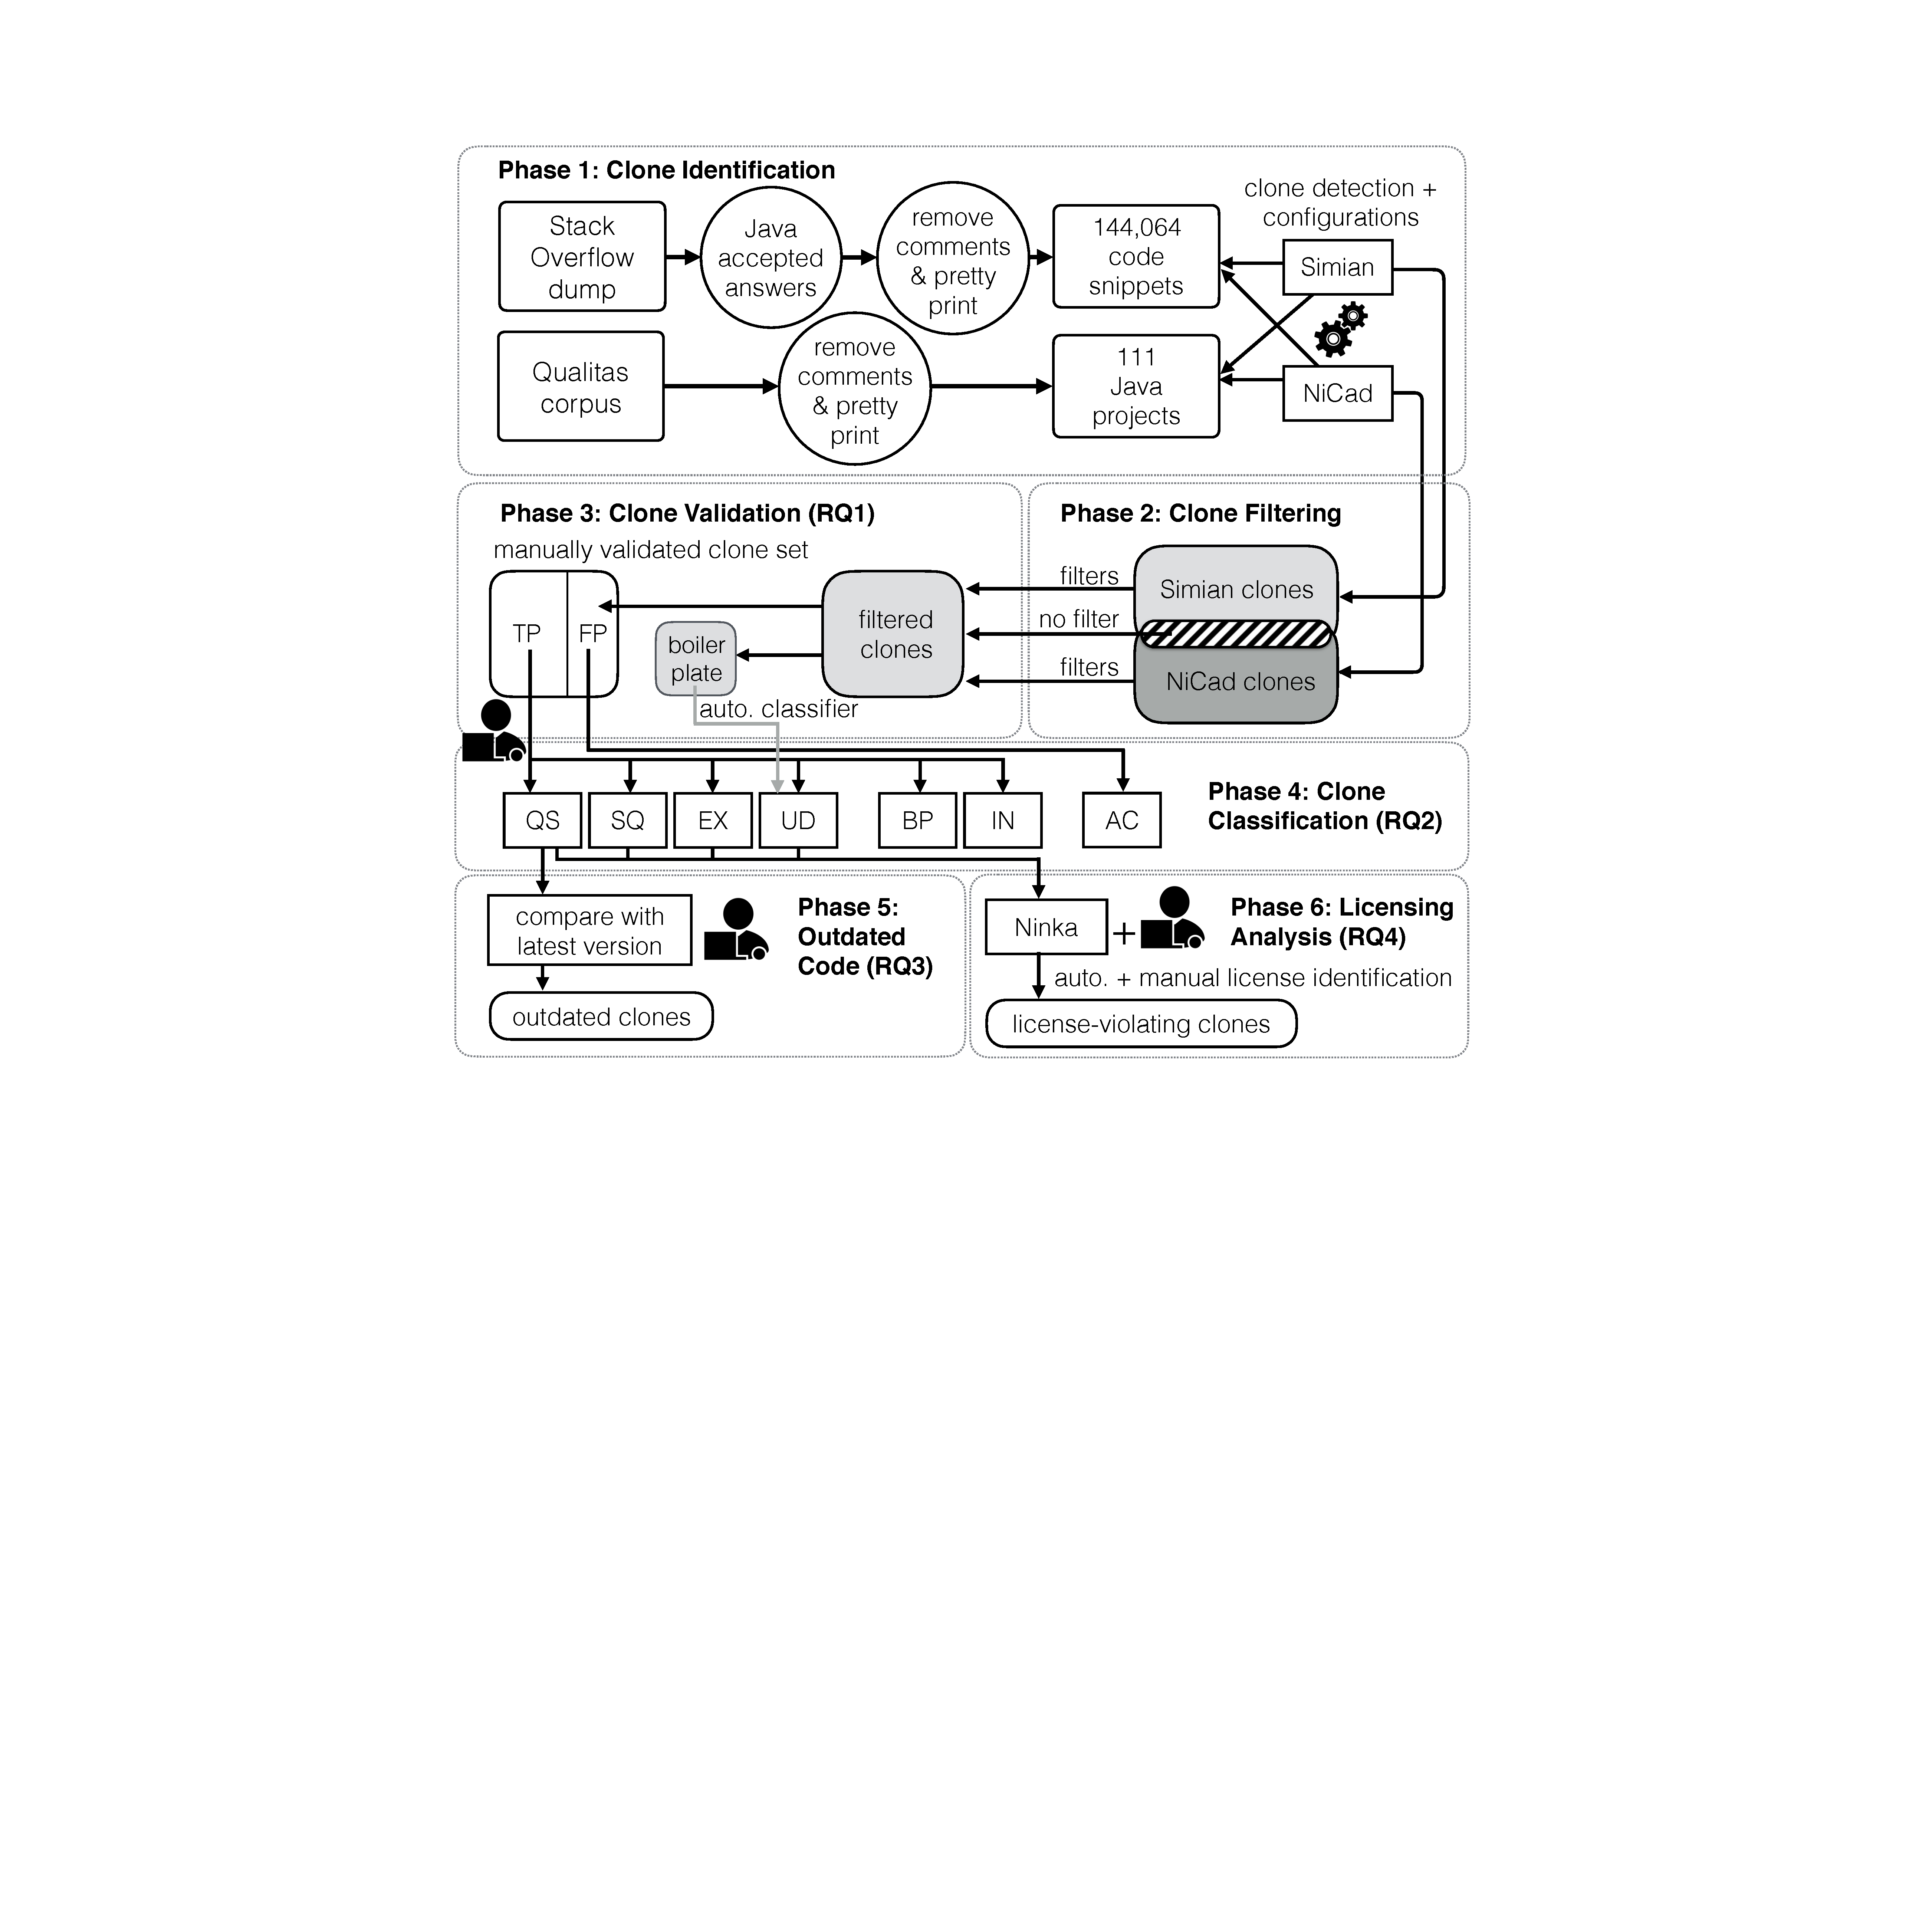
\includegraphics[width=\linewidth]{exp_framework_new}
	\caption{Experimental framework}
	\label{fig:exp_framework}
\end{figure}

%\subsection{Experimental Setup}
%\vspace{1ex}
To answer these five research questions, we perform an empirical study to
locate and study the online code clones between Stack Overflow and open source
projects. 
%
%\subsection{Methodology}
%
We designed our study in 6 phases as depicted in \Cref{fig:exp_framework} where
we build different data sets to answer each of our four research
questions. 

\subsection{Phase 1: Clone Identification}

We rely on two source data sets in this study: Java code snippets in answers
on Stack Overflow and open source projects from the Qualitas corpus
\cite{QualitasCorpus}.

\textbf{Stack Overflow:} 
We extracted Java code snippets from a snapshot of a Stack Overflow
dump\footnote{\url{https://archive.org/details/stackexchange}} in January 2016.
% The archived dump has a size of 9 gigabytes.
The data dump is in XML format containing information of posts (questions and
answers) and we were interested in code snippets embedded in posts which were
located between {\small\texttt{<code>}...\texttt{</code>}} tags. A Stack
Overflow thread contains a question and several answers. An answer can also be
marked as \textbf{accepted answer} by the questioner if the solution fixes
his/her problem. We collected Java code snippets using two criteria. First, we
only focused on code snippets in accepted answers. We chose the snippets in
accepted answers because they actually solved the problems in the questions.
Moreover, they are always displayed just below the questions which makes them
more likely to be reused than other answers. Second, we were only interested in
code snippets of at least ten lines. Although the minimum clone size of six
lines are usual in clone detection~\cite{Bellon2007,Wang2013,Koschke2006},
snippets of at least ten lines are usually more interesting since most of
boiler-plate code of \texttt{equal} or \texttt{hashCode} methods are removed.
Each snippet was extracted from the dump and saved to a file. Moreover, we
filtered out irrelevant code snippets that were part of the accepted answers
but were not written in Java by using regular expressions and manual checking.
~\FIXME{@Jens, should I mention I use PMD CPD to help here? More confusing?}.
Finally we obtained
72,365 Java code snippets containing 1,840,581 lines\footnote{Measured by cloc:
	\url{https://github.com/AlDanial/cloc}} of Java source code. The median of the
snippet size is 10.

\textbf{Open source systems: }
We selected the established \textbf{Qualitas} corpus~\cite{QualitasCorpus}. It is a curated Java corpus that has been used in several
software engineering
studies~\cite{Taube-Schock2011,Beckman2011,Vasilescu2011,Omar2012}. The
projects in the corpus represent various domains of software systems
ranging from programming languages to
visualisation. We selected the release 20130901r
of the Qualitas corpus containing 112 Java open source projects. This
release contains projects with releases no later than 1st September
2013. We intentionally chose an old corpus from 2013 since we are interested in
online code clones in the direction from open source projects to Stack
Overflow. The 20130901r snapshot provides Java code that is more than
2 years older than the Stack Overflow snapshot, which is sufficiently
long for a number of code snippets to be copied onto Stack Overflow
and also to observe if clones become outdated. Out of 112 Qualitas
projects, there is one project, \textsf{jre}, that does not contain
Java source code due to its licensing limitation~\cite{QualitasCorpus}
and is removed from the study. This resulted in 111
projects analysed in the study, for a total of 166,709 Java files containing 19,614,083
lines of code (see \Cref{tab:datasets}). The median project size is 60,667 lines of code.

\begin{table}
	\centering
	\caption{Stack Overflow and Qualitas datasets}
	\label{tab:datasets}
	%\small
	\begin{tabular}{lrrr}
		\toprule
		Dataset & No. of files & SLOC & Median \\
		\midrule
		Stack Overflow & 72,365 & 1,840,581 & ?? \\ 
		Qualitas &  166,709 & 19,614,083 & 60,667 \\ 
		\bottomrule
	\end{tabular} 
\end{table}

\textbf{Clone Detection Tools: } We use clone detection to discover online code
clones. %\textbf{Clone Detection and Configuration: }
There are a number of restrictions in terms of choosing the clone detection
tools for this study. The main restriction is due to nature of code snippets
posted on Stack Overflow, as most of them are incomplete Java classes or
methods. Hence, a detector must be flexible enough to process code snippets that
are not compilable or not complete blocks. Moreover, since the amount of code
that has to be processed is in a scale of millions line of code (as shown in
\Cref{tab:datasets}), a clone detector must be scalable enough to report clones
in a reasonable amount of time. We have tried 7 state-of-the-art clone detectors
including Simian~\cite{simian}, SourcererCC~\cite{Sajnani2016},
NiCad~\cite{Cordy,Roy2008}, CCFinder~\cite{Kamiya2002}, iClones~\cite{Gode2009},
DECKARD~\cite{Jiang2007a}, and PMD-CPD~\cite{pmd-cpd} against the Stack Overflow
and Qualitas datasets. NiCad failed to parse 44,960 Stack Overflow snippets
while PMD CPD failed to complete the execution due to lexical errors. iClones
could complete its execution but skipped 367 snippets due to malformed blocks in
Stack Overflow data set. CCFinder reported 8 errors while processing the two data set. 
Although Simian, SourcererCC, and DECKARD
could successfully report clones, we decided to choose only Simian and
SourcererCC due to their fast detection speed.

\textbf{Simian} is a text-based clone detector that locates clones at line-level
granularity and has been used extensively in several clone
studies~\cite{Ragkhitwetsagul2016, Wang2013, Mondal2011, Cheung2015,
	Krinke2010}. Furthermore, it offers normalisation of variable names and literals
(strings and numbers) which enables Simian to detect literal clones (type-1) and
parameterised clones (type-2). \textbf{SourcererCC} is a token-based clone
detector which detects clones at either function- or block-level granularity. It
can detect clones of type-1, -2 up to type-3 (clones with added and removed
statements) and offer scalability against large code
corpus~\cite{Sajnani2016,Saini2016,Yang2017}. Another benefit of SourcererCC is
its indexing and search processing allows us to detect code clones between two
systems. 

We prepared the Java code in both datasets by removing comments and
pretty-printing to increase the clone detection accuracy. Then, we deployed the
two detectors to locate clones between the two datasets.  For each Qualitas
project, we ran the tools on the project's code and the entire Stack Overflow
data. Due to incomplete code blocks and functions
normally found in Stack Overflow snippets, the built-in SourcererCC's Java
tokeniser could not parse 45,903 snippets, more than half of them. Nevertheless,
the tool provides an option to plug in a customised tokeniser, so we developed a
special Java tokeniser with assistance from the tool's creator. The customised
tokeniser successfully processed all Stack Overflow snippets.
Simian did not provide an option to detect cross-project clones. Hence the
Simian clone report was filtered to contain only clone pairs between Stack
Overflow and Qualitas projects, removing all clone pairs within either Stack
Overflow or within Qualitas. 

\begin{table}
	\centering
	\caption{Configurations of Simian and SourcererCC}
	\label{t:param_tuning}
%		\resizebox{\columnwidth}{!}{
%	\small
	\begin{tabular}{lp{5cm}}
		\toprule
		Tool & Configurations \\
		\midrule
		Simian~(\textit{S}) &  Threshold=10, ignoreStringCase, \newline ignoreCharacterCase, \newline ignoreModifiers \\ 
		\midrule
		SourcererCC~(\textit{SCC}) & Functions, Minimum clone size=10, \newline Similarity=80\% \\
		\bottomrule
	\end{tabular} %
%	}
\end{table}

\textbf{Clone Detection Configuration: } We are aware of effects of
configurations to clone detection results and the importance of searching for
optimised configurations in empirical clone
studies~\cite{Svajlenko2014,Wang2014,cr2016ssbse,Ragkhitwetsagul2016}. However,
considering the massive size of the two datasets and the search space of at
least 15 Simian and 3 SourcererCC parameters, we are unable to search for the
best configurations of the tools. Thus, we decided to configure Simian and
SourcererCC based on their established default configurations chosen by the
tools' creators. All variable renaming are disabled to decrease a number of
false positives since we aim for finding clones that are copied from open source
projects with minimal modifications. The two clone detectors complement each
other by having Simian detecting literal copies of code snippets and SourcererCC
detecting clones with added/deleted statments. We made sure that they 
detected only non-trivial clones by increasing the minimum clone size to ten
lines.
%(denoted as \textit{D}), and (2)~the discovered configurations for
%Bellon's Java projects from \textit{EvaClone}~\cite{Wang2013}, a study
%of optimising clone detectors' configurations based on clone agreement
%(denoted by \textit{E}). \Cref{t:param_tuning} shows the two configurations.
%In total, we have four configurations: Simian with the default
%configuration ($S_D$), Simian with the EvaClone configuration ($S_E$), 
%NiCad with the default configuration ($N_D$)
%and NiCad with the EvaClone configuration ($N_E$).

%We encountered NiCad failures with a few Qualitas projects.~$N_D$
%could not detect clones in \textsf{hibernate} due to clustering
%errors. $N_E$ generated errors during code normalisation for 5
%projects including \textsf{vuze}, \textsf{hibernate},
%\textsf{myfaces}, \textsf{netbeans}, and \textsf{spring}. We have
%contacted the creator of NiCad regarding the issues. They identified
%the issues as problems in the TXL grammar and as problems of long file
%paths, and will be fixed in the next NiCad releases.

The number of online clone pairs reported % by running Simian and NiCad
are presented in \Cref{tab:orig_stats}. Simian reports 721 clone
pairs while SourcererCC reports 1,678 clone pairs. 
SourcererCC reports more clones due to its capability of detecting
type-1 to type-3 clones while Simian only detects type-1 and type-2 clones.
The average clone size reported by Simian is
16.61 lines which is slightly smaller than SourcererCC (17.86 lines).

\begin{table}
	\centering
	\caption{Number of online clones reported by Simian and SourcererCC}
	\label{tab:orig_stats}
	%\small
	%\resizebox{\columnwidth}{!}{%
	\begin{tabular}{lrr}
		\toprule
		Stats & \multicolumn{1}{c}{Total clone pairs} & \multicolumn{1}{c}{Average clone size} \\
		\midrule
		Simian & 721 & 16.61 \\
		SourcererCC & 1,678 & 17.86 \\
		\bottomrule
	\end{tabular} %
	%}
\end{table}

\subsection{Phase 2: Clone Merging} As there are in total 315,786,118 clone
pairs reported, it is infeasible for humans to manually validate them all.
Instead of investigating a random sample, we adopted the idea of \textbf{clone
	agreement} which has been used in clone research studies~\cite{Funaro2010,
	Wang2013,cr2016ssbse} in situations where a clone oracle is missing or
impossible to establish. Clone pairs agreed by multiple clone detection tools
have a higher likelihood to be real clones~\cite{cr2016ssbse}. By using this
agreement-based approach, we reduced the number of clone candidates for manual
investigation and avoid a threat to internal validity of double counting the
same clone pair twice by merging the ones agreed by the two tools. To find
agreement between two clone pairs reported by two different tools, we used the
clone pair matching metric proposed by Bellon et al.~\cite{Bellon2007}. Two
clone pairs which have a large enough number of overlapping lines can be
categorised as either a good-match or an ok-match pair (denoted as \textit{good}
and \textit{ok} respectively) with a confidence value between 0 and 1. Although
good-match has stronger agreement than ok-match, we choose ok-match as our clone
merging method because it does not take clone size into account. Clone containment suits our
online code clones from two tools, Simian (line-level) and SourcererCC
(method-level), better because Simian's clone fragments  are sometimes smaller or bigger than
a method while SourcererCC's clone fragments are always confined to a method boundary.

\ We follow Bellon's original definitions of ok-match~\cite{Bellon2007}, which are based on how much two clone
fragments \textit{CF} is contained in each other:

%\squeezeup
%\begin{displaymath}
%overlap(\textrm{\textit{CF}}_1, \textrm{\textit{CF}}_2) = \frac{|lines(\textrm{\textit{CF}}_1) \cap lines(\textrm{\textit{CF}}_2)|}{|lines(\textrm{\textit{CF}}_1) \cup lines(\textrm{\textit{CF}}_2)|} 
%\end{displaymath}
% \squeezeup
\begin{displaymath}
contained(\textrm{\textit{CF}}_1, \textrm{\textit{CF}}_2) = \frac{|lines(\textrm{\textit{CF}}_1) \cap lines(\textrm{\textit{CF}}_2)|}{|lines(\textrm{\textit{CF}}_1)|}
\end{displaymath}
\noindent%
A clone pair \textit{CP} is formed by two clone fragments
\textit{CF$_1$} and \textit{CF$_2$}, i.e.~\textit{CP} =
(\textit{CF$_1$}, \textit{CF$_2$})
%, and the \textit{good-value} and
and the \textit{ok-value} of two clone pairs are defined as

%\squeezeup
%\begin{align*}
%good(\textrm{\textit{CP}}_1, \textrm{\textit{CP}}_2) = min(overlap(\textrm{\textit{CP}}_1.\textrm{\textit{CF}}_1,\textrm{\textit{CP}}_2.\textrm{\textit{CF}}_1), \\ overlap(\textrm{\textit{CP}}_1.\textrm{\textit{CF}}_2,\textrm{\textit{CP}}_2.\textrm{\textit{CF}}_2))
%\end{align*}
\begin{align*}
ok(\textrm{\textit{CP}}_1,\textrm{\textit{CP}}_2) = min(max(contained(\textrm{\textit{CP}}_1.\textrm{\textit{CF}}_1,\textrm{\textit{CP}}_2.\textrm{\textit{CF}}_1),~~ \\ contained(\textrm{\textit{CP}}_2.\textrm{\textit{CF}}_1,\textrm{\textit{CP}}_1.\textrm{\textit{CF}}_1)),~
\\ max(contained(\textrm{\textit{CP}}_1.\textrm{\textit{CF}}_2,\textrm{\textit{CP}}_2.\textrm{\textit{CF}}_2),~~ \\contained(\textrm{\textit{CP}}_2.\textrm{\textit{CF}}_2,\textrm{\textit{CP}}_1.\textrm{\textit{CF}}_2)))
\end{align*}

\noindent%
Two clone pairs $\textrm{\textit{CP}}_1$ and $\textrm{\textit{CP}}_2$
are called an \textit{ok-match(t)}  iff, for threshold $t \in [0,1]$ holds 
%\squeezeup
\begin{align*}
%good(\textrm{\textit{CP}}_1,\textrm{\textit{CP}}_2) & \geq t\\
ok(\textrm{\textit{CP}}_1,\textrm{\textit{CP}}_2) & \geq t
\end{align*}

Using the ok-match criteria with a predefined threshold \textit{t} of 0.7
similar to Bellon's study~\cite{Bellon2007}, we merge 721 clone pairs from
Simian and 1,678 clone pairs from SourcererCC into a single set of 2,302 online
clone pairs. There are 97 common clone pairs between the two clone sets 
as depicted in~\Cref{fig:clonemerging}.

\begin{figure}
	\centering
	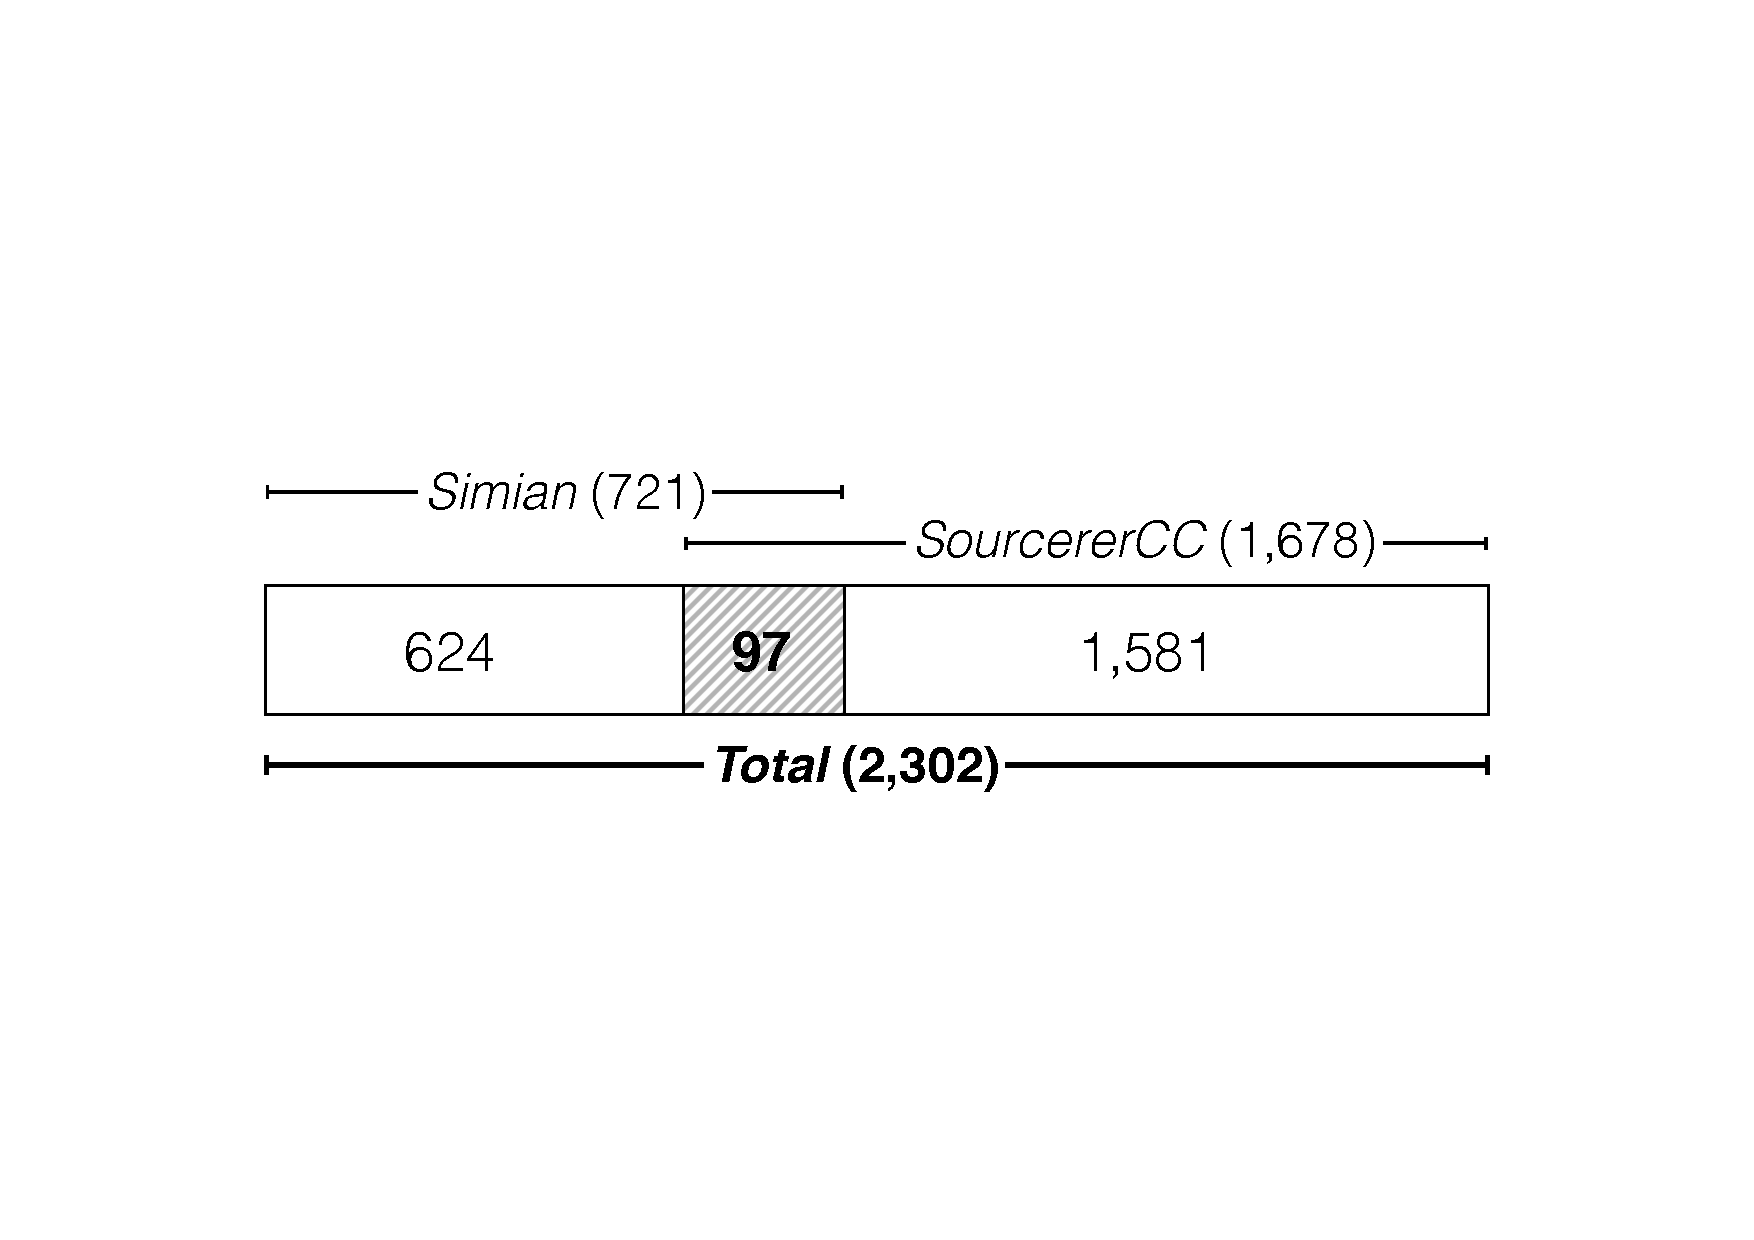
\includegraphics[width=0.8\linewidth]{clone_merging}
	\caption{The result from clone merging using Bellon's ok-match criterion}
	\label{fig:clonemerging}
\end{figure}

\subsection{Phase 3-4: Validation and Classification}
We used the 2,302 merged clone pairsfor
manual validation and classification.
The validation and classification of the pairs was done at the same time. 
The clone validation process (phase 3 in \Cref{fig:exp_framework}) involves checking 
if a clone pair is a true positive or a false positive. 
Moreover, we are also interested in 
the patterns of code cloning so we can gain more insights into 
how these clones are created (phase 4 in \Cref{fig:exp_framework}). 

\textbf{Manual investigation:} 
To mitigate the human error, we deployed two persons in the manual clone
investigation process. The first author, who is a research student working on
clone detection research for three years, and the third author, who is a
software engineering research student who is familiar with code clones, took the
role of the investigators performing a manual validation and classification of
the merged clone pairs. The two investigators separately went through each clone
pair candidate, looked at the clones, and decided if they are a true positive or
a false positive and classified them into an appropriate pattern. After the
validation, the results from the two investigators were compared and 607 (26\%)
conflicts were discussed and resolved. There are 145 conflicts caused by
one investigator being more careful than the other and finding evidence of 
copying while the other could not. They result in a better classification
to a stronger one, i.e.~from UD to QS or EX. 
%There were three conflicts where the two
%investigators could not find a consensus and the third author was involved for
%the final judgement.

% No. of conflicts = 37 (ok) + 352 (simian) + 218 (SCC)
% 33 pairs are changed from MP.UD --> CR.EX,QS
% 112 pairs are changed from CR.UD --> MP.EX,QS

\begin{table}
	\centering
	\caption{The seven patterns of online code cloning}
	\label{tab:classification_scheme}
	%\resizebox{\columnwidth}{!}{%
	\begin{tabular}{c@{~~}p{7.35cm}}
		\toprule
		Patt. & Description \\ 
		\midrule
		QS & Cloned from Qualitas project to Stack Overflow (Q $\rightarrow$ S). \\ 
		
		SQ &Cloned from Stack Overflow to Qualitas project (S $\rightarrow$ Q). \\ 
		
		EX & Cloned from an external source \textit{X} (X $\rightarrow$ S $\wedge$ X $\rightarrow$ Q). \\
		
		UD & Cloned from each other or from an external source \textit{X} outside the project (unknown) (S $\leftrightarrow$ Q $\vee$ (X $\rightarrow$ S $\wedge$ X $\rightarrow$ Q)). \\ 
		\midrule
		BP & Boiler-plate or IDE auto-generated \\ 
		
		IN & Inheritance, interface implementation  \\ 
		
		AC & Accidental similarity, false clones \\ 
		\bottomrule 
	\end{tabular}  %
	%}
\end{table}

\textbf{The online cloning classification patterns:} 
We studied the eight patterns of cloning from Kapser et
al.~\cite{Kapser2006,Kapser2008} and performed a preliminary study to
evaluate its applicability to our study. 
We tried to classify 697 online clone pairs from
the reported clones in phase 1 
%Using the $S_D$ clone report,
%snippets were ranked according to (1)~clone pair frequency,
%(2)~popularity (i.e.~number of associated Qualitas projects),
%(3)~clone size in SLOC, and (4)~ratio of cloned code per snippet. We
%selected these four criteria so that we could cover the online clones
%from various aspects. We selected the top 10 from each ranking and
%obtained 34 unique Stack Overflow snippets. The snippets were
%associated with 697 clone pairs.
%\subsection{Defining Online Code Cloning Patterns}
using Kapser's cloning patterns. We found that 
% the
% clone pairs were categorised into either Customisation or Templating.
% Thus, 
Kapser's patterns are too broad for our study and a
more suitable and fine-grained classification scheme is needed. After
a preliminary study, we adopted one of Kapser's cloning patterns,
\emph{boiler-plate code}, and defined
six new cloning patterns. The seven patterns include QS, SQ, EX, UD, BP,
IN, and AC as presented in \Cref{tab:classification_scheme}. Pattern
QS (\textbf{Q}ualitas to \textbf{S}tack Overflow) represents clones
that have evidence of being copied from a Qualitas project to Stack
Overflow. The evidence of copying can be found in comments in the
Qualitas source code or in the Stack Overflow post's contents. Pattern
SQ (\textbf{S}tack Overflow to \textbf{Q}ualitas) is cloning, with
evidence, in the opposite direction from Stack Overflow to a Qualitas
project. Pattern EX (\textbf{Ex}ternal Sources) is cloning that has
evidence of copying from a single or multiple external sources to
Stack Overflow and to a Qualitas project.  Pattern UD
(\textbf{U}nknown \textbf{D}irection) is cloning that creates
identical or highly similar clones between Qualitas and Stack Overflow
but where we could not find any attribution of copying.
Pattern BP (\textbf{B}oiler-\textbf{P}late) represents clones
containing boiler-plate (according to our definition of boiler-plate 
code in \Cref{tab:boiler-plate_code} which is more specific to Java
than the definition in Kapser's~\cite{Kapser2008}).
%of {\small\verb|equals()|} methods,
%getters/setters, well-known code patterns such as deleting a file
%or implementing a {\small{\texttt{toString}} method,
% or IDE-generated code such as GUI components. 
 Pattern
IN (\textbf{In}heritance/Interface) is cloning by inheritance of the
same super class or implementation of the same interface. These two
activities usually result in similar overriding methods. The last
pattern, AC (\textbf{A}ccidental \textbf{C}lones), represents
accidentally similar clone pairs. These are mainly false positive
clones from the clone detectors such as similar
{\small\texttt{try-catch}} statements.

\begin{table}
	\centering
	\caption{The definition of boiler-plate code}
	\label{tab:boiler-plate_code}
	\begin{tabular}{lp{5.5cm}}
		\toprule
		Type & Description \\ 
		\midrule
		\textbf{API constraints} & Similar code fragments are created because of a constraint by an API. For example, reading and writing to database using JDBC, reading and writing a file in Java. \\
		\midrule
		\textbf{Templating} & An optimised or stable code fragment is reused multiple times. This also includes auto-generated code by IDE. \\
		\midrule
		\textbf{Design patterns} & Java design patterns suggest a way of implementing similar pieces of code. For example, getters, setters, {\small\texttt{equals}}, {\small\texttt{hashCode}}, and {\small\texttt{toString}} method. \\
		\bottomrule 
	\end{tabular}  %
	%}
\end{table}

\begin{figure}
	\centering
	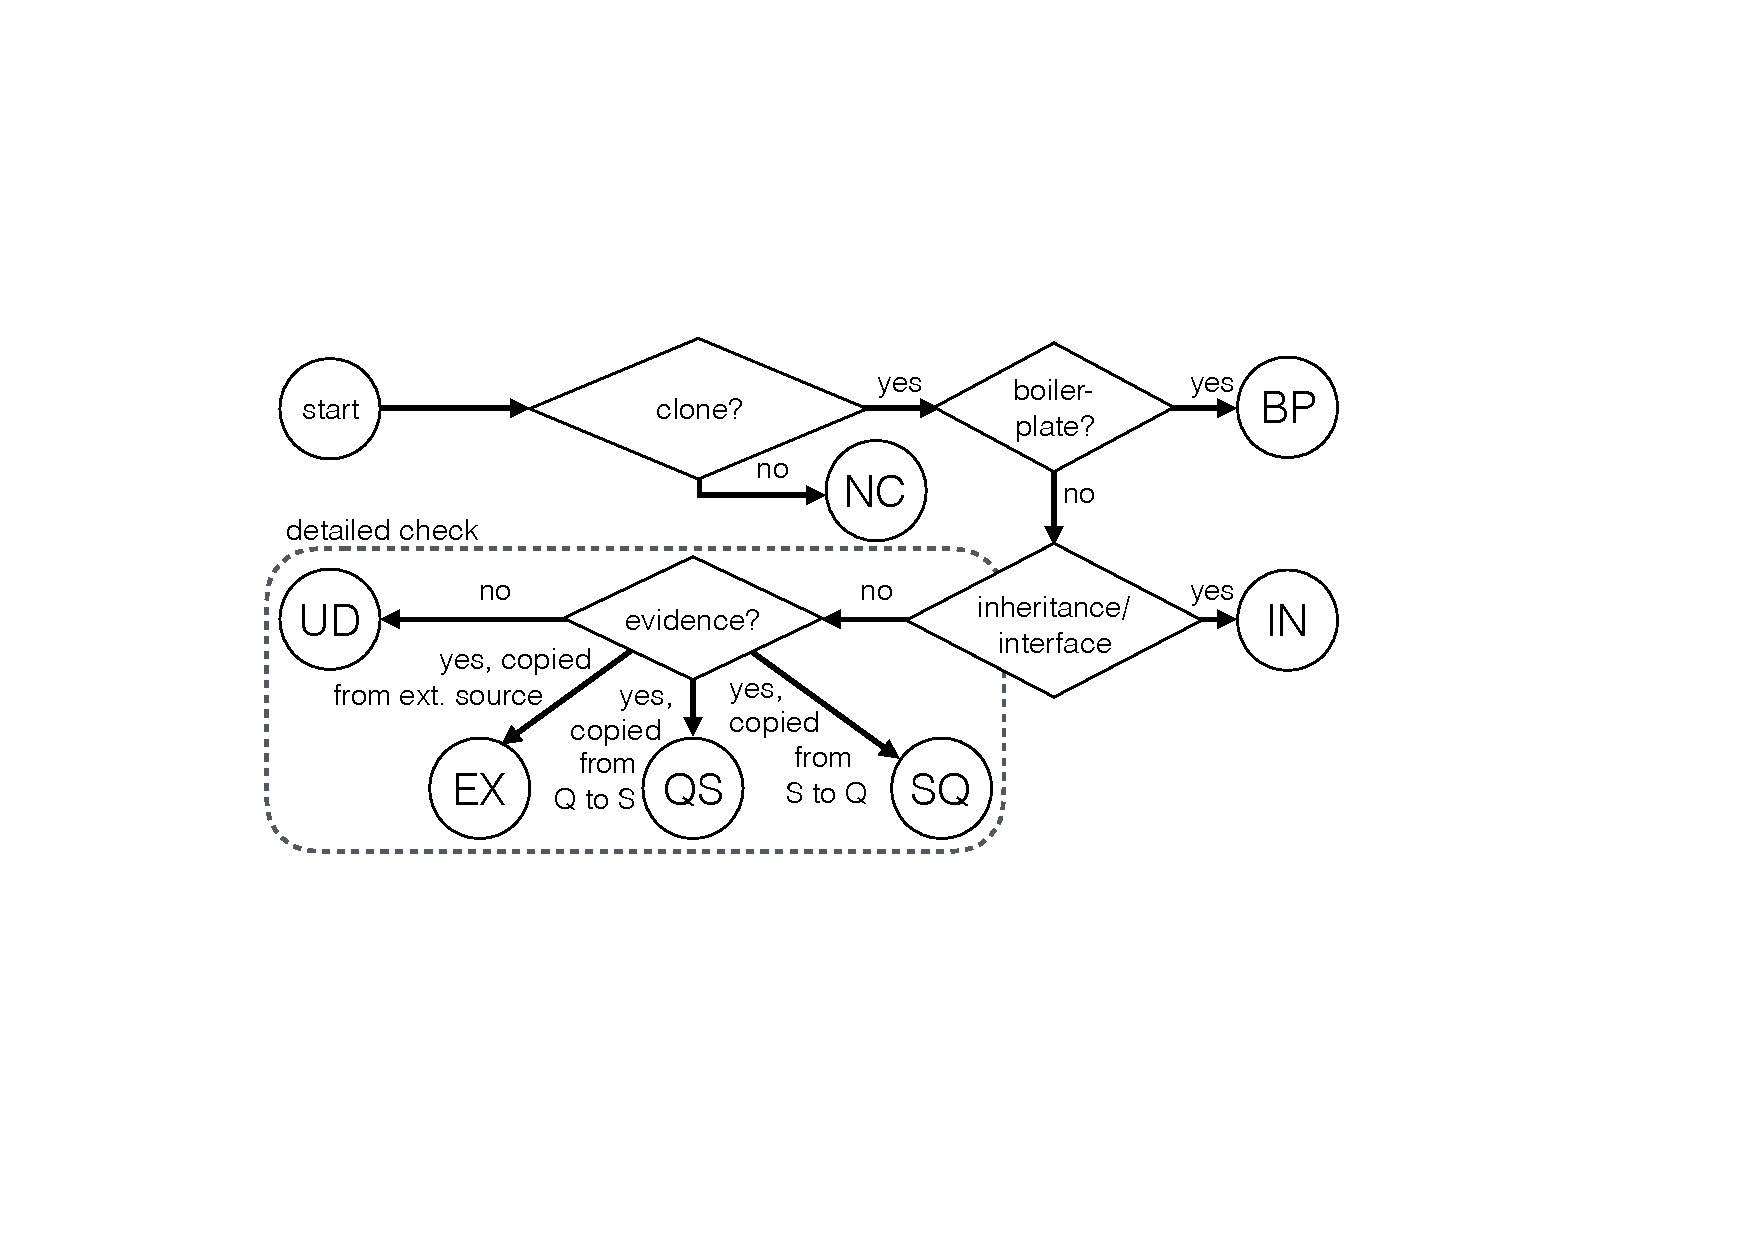
\includegraphics[width=0.9\linewidth]{classification_process}\vspace{-1ex}
	\caption{Online code clone classification process}
	\label{fig:classification_process}
\end{figure}

The classification of the filtered online clone pairs followed the steps
depicted in \Cref{fig:classification_process}. First, we look at a pair of clone
fragments to see their similarity. If they are accidentally similar clones after
code normalisation or false positive clones from the clone detection tools, we
classify the pair into \textbf{AC}. If the two fragments are boiler-plate code,
the pair is classified into \textbf{BP}. If they implement the same interface or
inherited the same class and share similar overriding methods, the pair is
classified into \textbf{IN}. If the pair is not \textbf{BP}, \textbf{IN}, or
\textbf{AC}, we start a detailed investigation. We check the corresponding Stack
Overflow post, read through it carefully and look for any evidence mentioning
code copying. If evidence of copying has been found from a Qualitas project, the
pair is classified in \textbf{QS}. In several occasions, we used extra
information such as questions' contents, name of posters, and tags to gain a
better understanding. On the other hand, if the source code from the Qualitas
project mentions copying from Stack Overflow, the pair is classified into
\textbf{SQ}. If there is evidence of copying from an external source instead of
a Qualitas projects, the pair is classified into \textbf{EX}. Lastly, if there
is no evidence of copying in any direction but the clone fragments are highly
similar, we classify them into \textbf{UD}.

\subsection{Phase 5: Outdated Clones} Outdated code occurs when a piece of code
has been copied from its origin to another location and later the original has
been updated~\cite{Xia2014}. Usually code clone detection is used to locate
clone instances and update them to match with the originals~\cite{Bellon2007}.
However, online code clones are more difficult to detect than in regular
software projects due to its large search space and a mix of natural and
programming languages combined in the same post.

To search for outdated online code clones, we focused on the \textbf{QS} clone
pairs that were cloned from Qualitas to Stack Overflow and compared them with
their latest versions. We downloaded the latest version of the Qualitas projects
from their repositories on October 3, 2017. For each \textbf{QS} online clone
pair, we used the clone from Qualitas as a proxy. We searched for its latest
version by the file name and located the cloned region in the file based on the
method name or specific code statements. We then compared the Stack Overflow
snippet to its latest version line-by-line to find if any change has been made
to the source code. We also made sure that the changes did not come from the
modifications made to the Stack Overflow snippets by the posters but from the
updates in the projects themselves. When we found inconsistent lines between the
two versions, we used {\small\texttt{git blame}} to see who modified those lines
of code and the timestamps. We also collected IDs of issue tracking information
if the code change is linked to an automatic issue tracking system, such as Jira.

\subsection{Phase 6: Licensing Analysis} Software licensing plays an important
role in software development. Violation of software licenses impacts software
delivery and also leads to legal issues~\cite{Sprigman2015}. 
One can run into a licensing issue if one integrates third-party source code
into their software without checking. A study by An et al.~\cite{An2017} reports
1,279 cases of potential license violations between 399 Android apps and Stack
Overflow code snippets.

We analysed licensing conflicts of the online clones in the \textbf{QS},
\textbf{EX}, and \textbf{UD} set. The licenses were extracted by \emph{Ninka},
an automatic license identification tool~\cite{German2010}. Since Ninka works at
file level, we report the findings based on Stack Overflow snippets and Qualitas
source files instead of the clone pairs (duplicates were ignored). For the ones
that could not be automatically identified by Ninka and have been reported as
{\small\texttt{SeeFile}} or {\small\texttt{Unknown}}, we looked at them manually
to see if any license can be found.

\subsection{Stack Overflow Developers' Survey} We support our findings of
outdated and license-violating code snippets on Stack Overflow by asking Stack
Overflow users to take an online survey. The survey was used for assessing awareness of
the developers on the two issues of outdated code and licensing-violating code
snippets. We designed the survey using Google Forms by following the guidelines by Pfleeger and
Kitchenham~\cite{Pfleeger2001,Kitchenham2002}. The survey was completely
anonymous and the participants could decide to leave at any time. It contained
11 questions. There were 7 Likert's scale questions, 3 yes/no questions, and one
open-ended question for additional comments. The first two questions were
mandatory while the other 9 questions were shown to the participants based on
their previous answers. The full survey can be found in our research note~
\FIXME{add URL to the RN}.


\begin{table}
	\centering
	\caption{The two groups of Stack Overflow users invited to take the survey}
	\label{tab:survey_target}
	\begin{tabular}{lrrrr}
		\toprule
		Target group & Reputation & Sent emails & Answers & Rate \\
		\midrule
		Group 1 & 963,731--7,674 & 300 & 112 & 37\% \\
		Group 2 & 7,636--6,999 & 307 & 85 & 28\% \\
		\bottomrule
	\end{tabular}
\end{table}

We selected the participants for our survey based on the users' reputations. On
Stack Overflow, a user's reputation reflects how much the community trust the
user. A user earns reputations when he or she receives up votes for good
questions and useful answers. Accepted answers receive more reputation score
than questions, and regular answers\footnote{Stack Overflow
	Reputation:~\url{https://stackoverflow.com/help/whats-reputation}}. Thus, Stack
Overflow reputation is an indicator of user's skills and their involvement in
asking and answering questions on the site. We call Stack Overflow users who
have high reputations ``Stack Overflow answerers.''

The participants were invited to take the survey via email addresses on their
public Stack Overflow and GitHub profiles. We selected the answerers who had highly
ranked all-time reputations\footnote{Stack Overflow Users (data as of 25 July
	2017):~\url{https://stackoverflow.com/users?tab=Reputation&filter=all}} and
separated them into two groups (see \Cref{tab:survey_target}) so that we can
compare the results or observe similar patterns between them. 
The first group had reputation from 963,731 (the
highest) to 7,674, and the second group had reputation from 7,636 to 6,999 which
we sent out 300 and 307 emails (excluding undelivered ones) respectively. The
survey was open for participation for two months, from 25 August 2017 to 25 August
2017, before we collected and analysed the responses.

\section{Results and Discussion}

We followed the 6 phases in the experimental framework (\Cref{fig:exp_framework})
to answer our four research questions. 
To answer RQ1, we rely on the number of manually validated true positive online clone pairs
in phase 3. We use the results of the manual classification by the
seven patterns of online code cloning to answer RQ2 (phase 4). 
For RQ3, we looked at the true positive clone pairs that are classified 
as clones from Qualitas to Stack Overflow and
checked if they have been changed after cloning (phase 5). Similarly, for RQ4, we looked at the license of each clone in the pattern 
QS, EX, UD and checked for a possibility of licensing violation (phase 6).

\subsection{RQ1: Online Code Clones} 

The statistics on clones obtained from the merged clone data set are
presented in \Cref{tab:snippets}. Simian and SourcererCC
reported clones in 460 snippets, approximately 0.6\% of the
72,365 Stack Overflow snippets, associated with 59 Qualitas
projects. For the cloned Stack Overflow snippets, the
average ratio of cloned code is 53.10\%.
% A quick manual check of Simian's clone report revealed that there
% were 11 problematic snippets. These 11 snippets triggered Simian to
% generate large clone clusters containing a huge number of false
% clones from array initialisation. Hence, their clones were removed
% from further analyses.

% \FIXME{Do you think we should report at this level or in more details 
% 	into $S_D$--$N_D$, $S_D$--$N_E$, $S_E$--$N_D$, $S_E$--$N_E$??}
% I don't think there is a need.

\begin{table}
	\caption{Investigated online clone pairs and corresponding snippets
		and Qualitas projects}
	\label{tab:snippets}
	\centering
	\begin{tabular}{p{2.2cm}rrrr}
		\toprule
		Set & Pairs & Snippets & Projects & Cloned ratio \\
		\midrule
		Reported clones & 2,302 & 460 & 59 & 53.10\% \\ 
		\midrule
		TP from manual validation & 2,076 & 443 & 59 & 53.89\% \\ 
		\bottomrule
	\end{tabular}
\end{table}

During the manual investigation of 2,302 clone pairs, we identified 226 pairs
as being accidental clones (AC), i.e.~false positives. After removing
them, the set still contains 2,076 true positive clone pairs between 443 Stack
Overflow snippets and 59 Qualitas projects. The average cloned ratio for the
true positive clone pairs is 53.89\%.

\textbf{To answer RQ1, we found more than half of Qualitas projects to share
	similar code with Stack Overflow code snippets. In the manually confirmed 
	data set of 2,302 clone pairs, we found 2,076 pairs as true positives which 
	account for 59 Qualitas projects and
	443 Stack Overflow code snippets.}

\subsection{RQ2: Patterns of Online Code Cloning}

We performed a manual classification
of the 2,302 merged clone pairs by following the classification process
in \Cref{fig:classification_process}. 
The classification results are shown in \Cref{tab:classification_good_o} 
and explained in the following.

\begin{table*}
	\centering
	\caption{Classifications of online clone pairs.}
	\label{tab:classification_good_o}
	%\small
	%\resizebox{\columnwidth}{!}
\end{table*}

\textbf{QS: Qualitas $\rightarrow$ Stack Overflow.} We found 248 online clone
pairs with evidences of cloning from Qualitas projects to Stack Overflow.
However, we observed that, in some cases, a cloned code snippet on Stack
Overflow matched with more than one code snippet in Qualitas projects. This is
because there were also code cloning inside Qualitas projects themselves. To
avoid double counting of such online clones, we consolidated clone pairs having
the same Stack Overflow snippet, starting line, and ending line into a single
clone pair. We finally obtained 154 QS pairs having unique Stack Overflow code
snippets and associated with 23 Qualitas projects listed in
\Cref{tab:qs_qualitas_projects}. The most cloned projects are \textsf{hibernate}
and \textsf{spring} with 24 clone pairs, followed by \textsf{eclipse} (21
pairs), \textsf{jung2} (19 pairs), \textsf{spring} (17 pairs), and
\textsf{jfreechart} (13 pairs). The clones are used as examples and are very
similar to their original Qualitas code with limited modifications. Most of them
have a statement in the Stack Overflow post saying that the code is ``copied'',
``borrowed'' or ``modified'' from a specific file or class in a Qualitas
project. For example, according to the motivating example in
\Cref{fig:before-after}, we found evidence in the Stack Overflow Post 22315734
saying that \textit{``Actually, you can learn how to compare in Hadoop from
	WritableComparator. Here is an examle that borrows some ideas from it.''}

\begin{table}
	\centering
	\caption{Qualitas projects associated with QS and UD online clone pairs}
	\label{tab:qs_qualitas_projects}
	%\small
	%\resizebox{\columnwidth}{!}{%
	\begin{tabular}{lrlr}
		\toprule
		\multicolumn{2}{c}{QS} & \multicolumn{2}{c}{UD} \\
		\midrule
		Project & Pairs & Project & Pairs\\
		\midrule
		hibernate & 24 & netbeans & 11 \\
		eclipse & 21 & eclipse & 8 \\
		jung2 & 19 & jstock & 5 \\
		spring & 17 & compiere & 5 \\
		jfreechart & 13 & ireport & 4 \\
		hadoop & 10 & jmeter & 4 \\
		log4j & 8 & jung2 & 3 \\
		tomcat & 8 & jhotdraw & 3 \\
		struts & 5 & c-jdbc & 3 \\
		lucene & 4 & log4j & 3 \\
		weka & 4 & wct & 2 \\
		junit & 3 & hibernate & 2 \\
		poi & 3 & tomcat & 2 \\
		compiere & 2 & spring & 1 \\
		jasperreports & 2 & rssowl & 1 \\
		jboss & 2 & mvnforum & 1 \\
		jgraph & 2 & jfreechart & 1 \\
		jstock & 2 & jboss & 1 \\
		antlr & 1 & hadoop & 1 \\
		itext & 1 & geotools & 1 \\
		jgrapht & 1 & freemind & 1 \\
		ant & 1 & findbugs & 1 \\
		c-jdbc & 1 & cayenne & 1 \\
		\bottomrule
	\end{tabular} 
	%}
\end{table}

\textbf{SQ: Stack Overflow $\rightarrow$ Qualitas.} We found one pair with
evidence of cloning from Stack Overflow post ID 698283 to
{\small\texttt{POIUtils.java}} in \textsf{jstock} project. The user
\textsf{yccheok} who asked the question in Stack Overflow is the author of
\textsf{jstock}. The question is about determining the right method to call
among 7 overloading methods of {\small\texttt{setCellValue}} during runtime. We
could not find evidence of copying or attribution to Stack Overflow in
\textsf{jstock}. However, considering that the 25 lines of code of
{\small\texttt{findMethodToInvoke}} method depicted in \Cref{fig:jstock_code} in Stack
Overflow is identical to the code in \textsf{jstock} including comments, it is almost certain that
the two code snippets form a clone pair. In addition, Stack Overflow answer was
posted on March 30, 2009, while the code in {\small\texttt{POIUtils}} class in
\textsf{jstock} was committed to GitHub on the next day of March 31, 2009.

\begin{figure}
	\begin{lstlisting}
private Method findMethodToInvoke(Object test) {
  Method method = parameterTypeMap.get(test.getClass());
  if (method != null) {
    return method;
  }

  // Look for superclasses
  Class<?> x = test.getClass().getSuperclass();
  while (x != null && x != Object.class) {
    method = parameterTypeMap.get(x);
    if (method != null) {
      return method;
    }
    x = x.getSuperclass();
  }

  // Look for interfaces
  for (Class<?> i : test.getClass().getInterfaces()) {
    method = parameterTypeMap.get(i);
    if (method != null) {
      return method;
    }
  }
  return null;
}
	\end{lstlisting}\vspace{-2ex}
	\caption{The {\small\texttt{findMethodToInvoke}} that is found to be copied from Stack Overflow post 698283 to {\small\texttt{POIUtils}} class.}
	\label{fig:jstock_code}
\end{figure}

We did not find other online clones besides the one mentioned above. 
This very low number of SQ clone pair is very likely due to the age of the
Qualitas corpus as another study~\cite{An2017} showed the presence of clones
from Stack Overflow in newer open source data sets. This is expected and
comes from our experimental design since
we are more interested in a cloning direction from Qualitas to Stack Overflow.

\begin{figure}
	\centering
	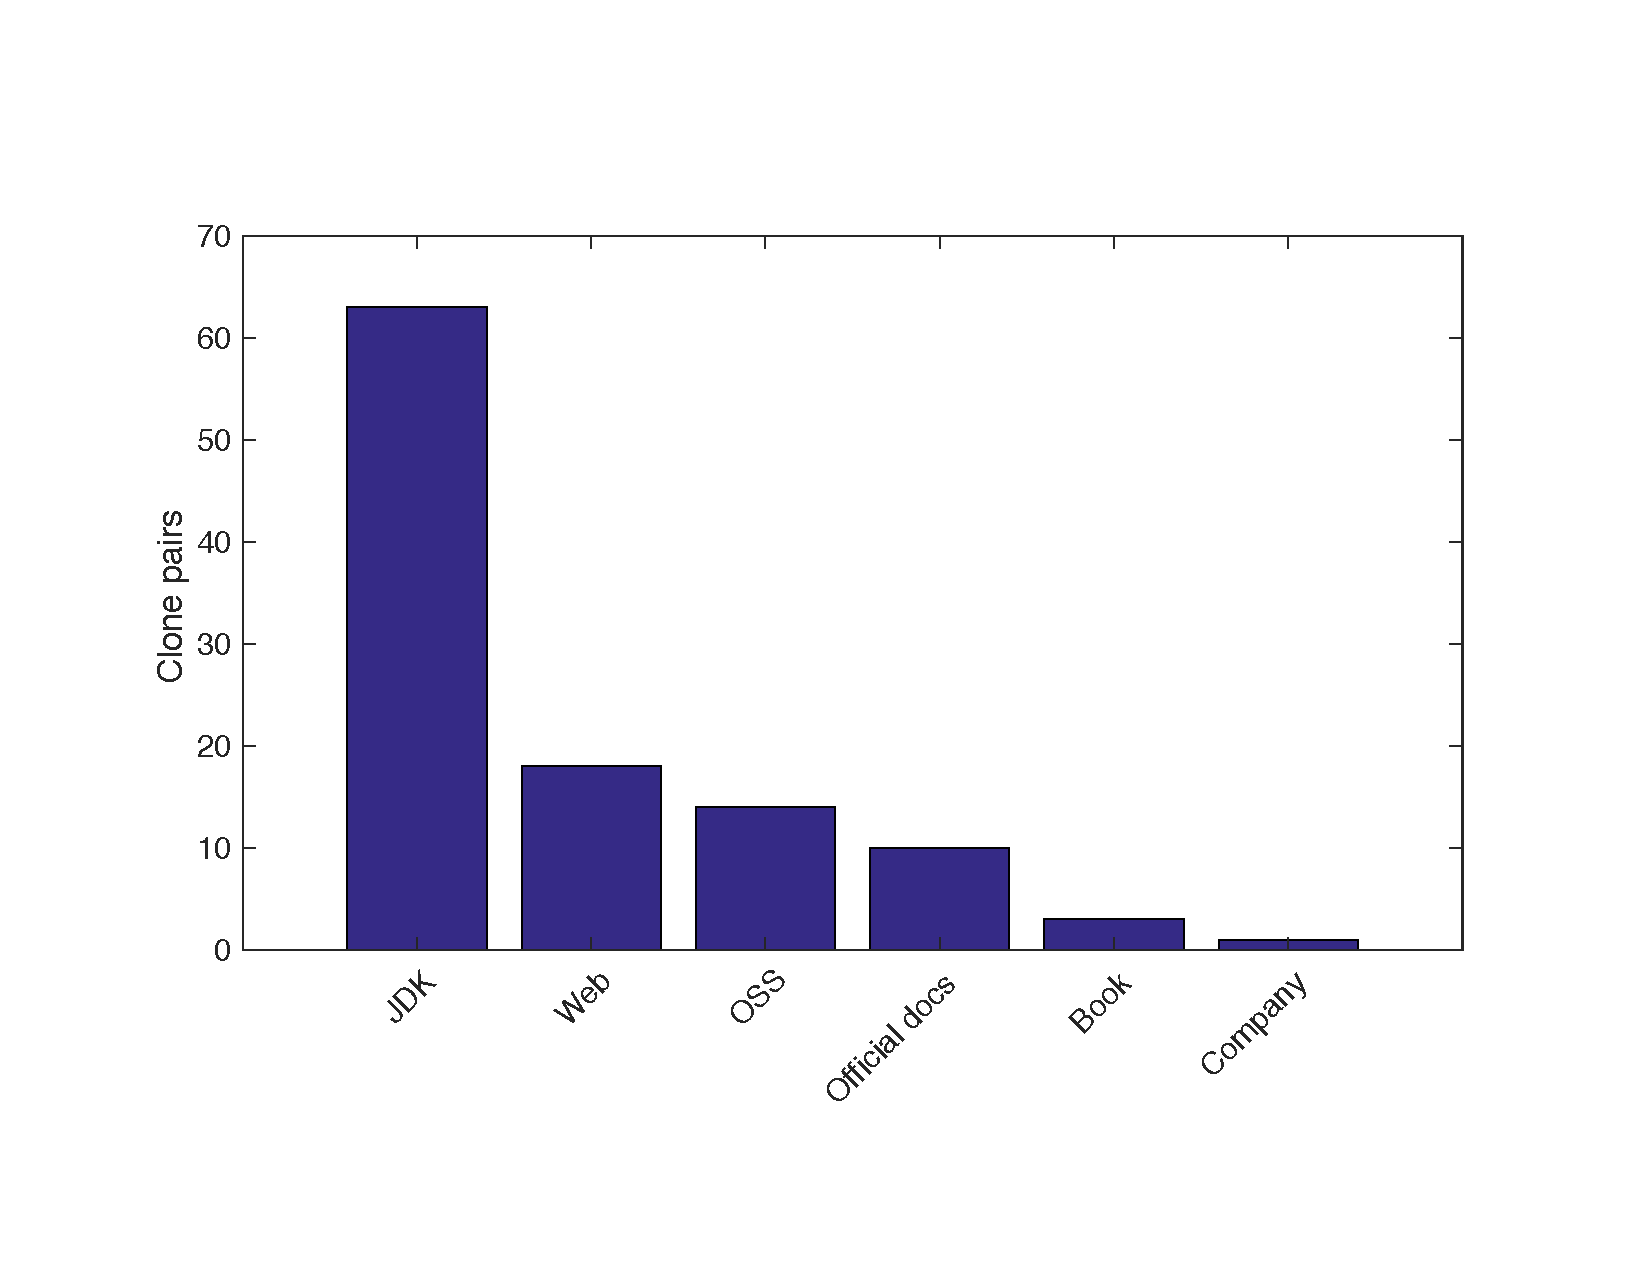
\includegraphics[width=0.9\linewidth]{ex_sources}
	\caption{Original sources of EX clone pairs}
	\label{fig:ex_sources}
\end{figure}

\textbf{EX: External Sources.} We found 199 clone pairs with evidence of cloning
from external sources to Stack Overflow. After getting rid of duplicated SO
snippets due to multiple intra-clone instances in Qualitas, we obtained 111 EX
pairs. Fifty pairs provide evidences of copying to both Stack
Overflow and Qualitas while the rest (61) only provides evidence of copying to
Stack Overflow. All of them contain statements giving an external source of the
cloned code which fall into six groups as displayed in \Cref{fig:ex_sources}. 
We discovered that 63 EX online clone pairs are copied from source code of classes or 
methods in Java SDK, 18 pairs are from websites, 15 pairs are from open source systems,
11 pairs are from Java official documentations from Sun Microsystems or Oracle,
3 pairs are from books, and 1 pair is from a company project.
For example, Stack Overflow Post
9549009 contains a code comment saying \textit{``Copied shamelessly from
	org.bouncycastle.crypto.generators.PKCS5S2ParametersGenerator''} which is an
open source project. Post 92962 includes a {\small\texttt{VerticalLabelUI}}
class with a license statement showing that it is developed by a private company
called \textsf{Sapient}. Post 12879764 has a text saying \textit{``Code modified
	and cleaned from the original at Filthy Rich Clients.''} which is a book for
developing animated and graphical effects for desktop Java applications. Another
example is a copy of code from a website in post 15260207. The text surrounding
source code reads ``\textit{I basically stole this from the web and modified it
	slightly... You can see the original post here
	(\url{http://www.java2s.com/Code/Java/Swing-JFC/DragListDemo.htm}).}''.
Interestingly, the code is actually a copy from Sun Microsystems.

\begin{table*}
	\centering
	\caption{Examples of the outdated QS online clones}
	\label{tab:stale_code_details}
	\resizebox{\linewidth}{!}{
		\begin{tabular}{cc|lcp{4cm}@{}rrc|lc@{}c}
			\toprule
			\multicolumn{2}{c|}{Stack Overflow} & \multicolumn{6}{c|}{Qualitas} & \multicolumn{3}{c}{Changes} \\ 
			\midrule
			Post & Date & Project & Ver. & File & Start & End & Date & Issue ID & Type$^*$ & Date \\
			\midrule
			2513183 & 25-Mar-10 & eclipse & 4.3 & GenerateToStringAction.java & 113 & 166 & & Bug 439874 & \textit{S} & 17-Mar-15 \\
			22315734 & 11-Mar-14 & hadoop & 1.0.0 & WritableComparator.java & 44 & 54 & 25-Aug-11 & HADOOP-11323 & \textit{S} & 20-Nov-14 \\
			23520731 & 7-May-14 & hibernate & 4.2.2 & SchemaUpdate.java & 115 & 168 & 22-May-13 & HHH-10458 & \textit{S} & 5-Feb-16 \\
			18232672 & 14-Aug-13 & log4j & 1.2.16 & SMTPAppender.java & 207 & 228 & & Bug 44644 & \textit{R} & 18-Oct-08 \\ 
			17697173 & 17-Jul-13 & lucene & 4.3.0 & SlowSynonymFilterFactory.java & 38 & 52 & & LUCENE-4095 & \textit{D} & 31-May-12 \\
			21734562 & 12-Feb-14 & tomcat & 7.0.2  & FormAuthenticator.java & 51 & 61 & 4-Aug-10 & BZ 59823 &\textit{R} & 4-Aug-16 \\
			12593810 & 26-Sep-12 & poi & 3.6 & WorkbookFactory.java & 49 & 60 & 7-Dec-09 & 57593 & \textit{R} & 30-Apr-15 \\
			8037824 & 7-Nov-11 & jasperreports & 3.7.4 & JRVerifier.java & 1221 & 1240 & 31-May-10 & N/A & \textit{D} & 20-May-11 \\
			3758110 & 21-Sep-10 & spring & 3.0.5  & DefaultAnnotation\newline HandlerMapping.java & 78 & 92 & 20-Oct-10 & SPR-14129 & \textit{D} & 20-Jan-12 \\
			14019840 & 24-Dec-12 & struts & 2.2.1 & DefaultActionMapper.java & 273 & 288 & & WW-4225 & \textit{S} & 18-Oct-13 \\
			\bottomrule 
			\multicolumn{10}{l}{{\footnotesize * \textit{S}:
					modified/added/deleted statements, \textit{D}: file
					has been deleted,  \textit{R}: method has been
					rewritten completely}}
		\end{tabular} %
	}
\end{table*}

These findings complement a study of clones between software
projects~\cite{Svajlenko2014}. We found that cloning can also happen among
different sources on the Internet just like software projects. The are 18 clone
pairs that originated from programming websites including \url{www.java2s.com}
and \url{exampledepot.com}. Moreover, there is one snippet which comes from a
research website. We found that a snippet to generate graphical \textit{Perlin
	noise} is copied from NYU Media Research Lab
(\url{http://mrl.nyu.edu/~perlin/noise/}) website and is used on Stack Overflow
and in the \textsf{aoi} project with attribution. There are other EX pairs which
are copied from open source libraries or Java SDK such as \textsf{Mozilla
	Rhino}, \textsf{java.util}, \textsf{javax.swing}, \textsf{javax.servlet}, and
the \textsf{bouncycastle} cryptography project.

\textbf{UD: Unknown Direction.} We found 107 online clone pairs, reduced to 65
pairs after consolidating the clones, with no evidence of cloning between Qualitas
and Stack Overflow but with a high code similarity that suggests cloning. 
The most cloned projects is \textsf{netbeans} with 11 clone pairs. Most of the
clones are a large chunk of code handling GUI components. Although these GUI
clones might be auto-generated by IDEs, we did not find any evidence. The second
most cloned project is \textsf{eclipse} (8 pairs), followed by \textsf{jstock},
a free stock market software, and \textsf{compiere}, a software and customer
relationship management (CRM) system, (5 pairs).

\textbf{BP: Boiler-Plate.} There were a large amount of boiler-plate clone pairs
found in this study. We observed 1,505 such clone pairs and 217 after
consolidation. The BP clone pairs account for 65\% of all clone pairs we
classified. The majority of them are {\small{\texttt{equals()}}} methods.

\textbf{IN: Inheritance/interface.} There were 16 clone pairs, 9 pairs after
consolidation, found to be similar because they implement the same interface or
inheriting from the same class. An example is the two implementations of a
custom data type which implements {\small\texttt{UserType}}. They share similar
{\small\texttt{@Override}} methods of {\small\texttt{deepCopy}},
{\small\texttt{isMutable}}, {\small\texttt{assemble}},
{\small\texttt{disassemble}}, and {\small\texttt{replace}}.

\textbf{AC: Accidental Clones.} There were 226 accidental clone
pairs, 53 after consolidation. Mainly, they are false positive clones caused by code
normalisation and false type-3 clones from SourcererCC. 
Examples of the AC clone instances include {\small\texttt{finally}} or
{\small\texttt{try-catch}} clauses that were accidentally the same due
to their very small sizes, and similar {\small\texttt{switch-case}}
statements.

\textbf{To answer RQ2, we found 154 pairs with
	strong evidences to be cloned from 23 Qualitas projects to Stack Overflow, 1 pair
	was cloned from Stack Overflow to Qualitas, and
	111 pairs were found to be cloned to Stack Overflow from external
	sources. However, the largest amount of the clone pairs
	between Stack Overflow and Qualitas projects are \linebreak boiler-plate code
	(217), followed by 65 clone pairs with no evidence that the code has actually been copied,
	and 16 pairs of clones due to implementing the same interface or inheriting the same class.} 


\subsection{RQ3: Outdated Online Code Clones}

\begin{figure*}
	\centering
	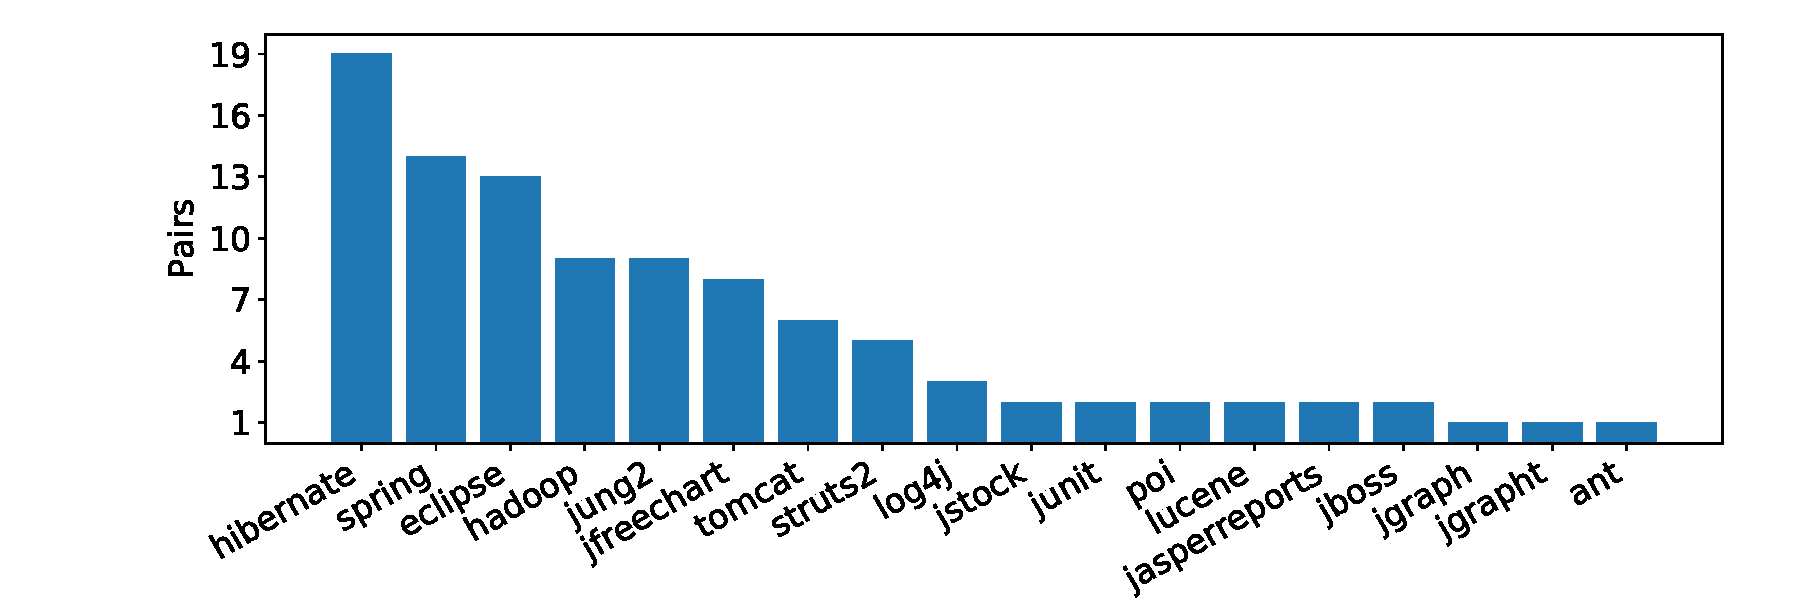
\includegraphics[width=0.8\linewidth]{outdated}
	\caption{Outdated QS online clone pairs group by projects}
	\label{fig:outdated}
\end{figure*}

We discovered 101 outdated online clone pairs out of 154 pairs. As shown in
\Cref{fig:outdated}, \textsf{hibernate} has the highest number of 19 outdated
pairs, followed by 14 from \textsf{spring}, 13 from \textsf{eclipse}, and 9 from
\textsf{hadoop}. Besides the two examples of outdated code in % \textsf{hadoop}'s
{\small{\texttt{WritableComparator.java}}} and
{\small{\texttt{StringUtils.java}}} from \textsf{hadoop} shown in
\Cref{fig:before-after} and \Cref{fig:before-after_2}, we also found a few
outdated code elements which contained a large amount of modifications. For
example, the code snippet in Stack Overflow post 23520731 is a copy of
{\small{\texttt{SchemaUpdate.java}}} in \textsf{hibernate}. The code has been
heavily modified on February 5, 2016.

%\begin{figure}
%	\centering
%	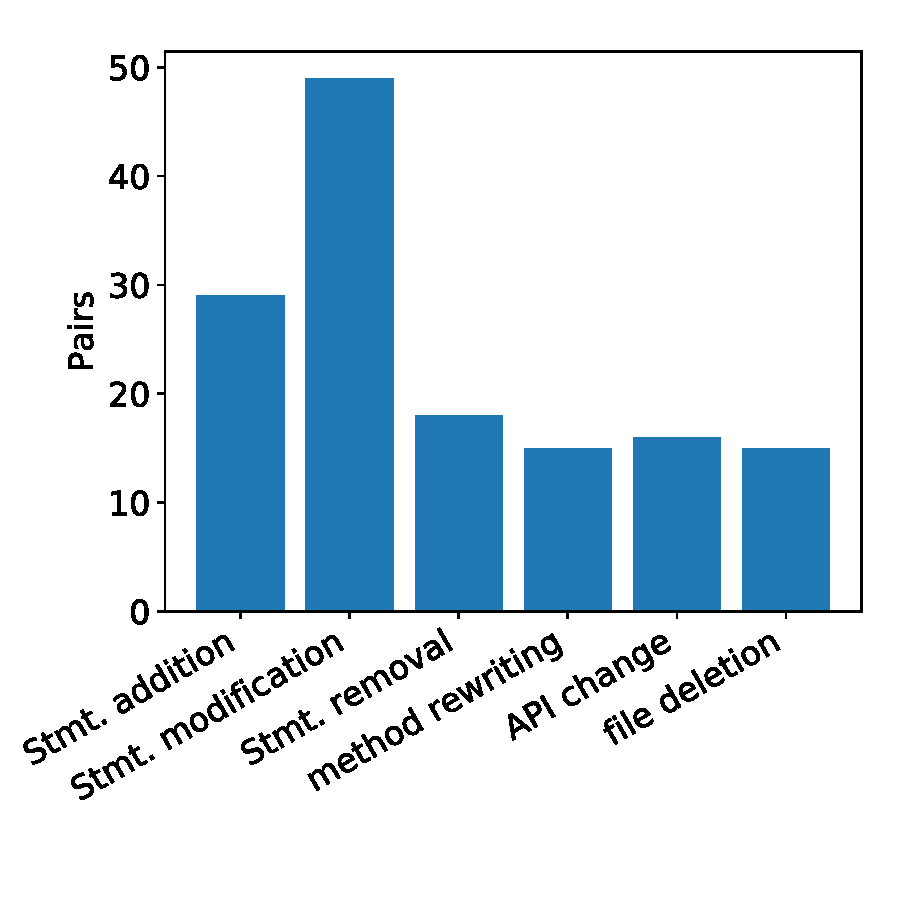
\includegraphics[width=0.7\linewidth]{mod_types}
%	\caption{Six code modification types found when comparing the outdated clone pairs to their latest versions}
%	\label{fig:mod_types}
%\end{figure}

\begin{table}
	\centering
	\caption{Six code modification types found when comparing the outdated clone pairs to their latest versions}
	\label{tab:mod_types}
		\begin{tabular}{lr}
			\toprule
			Modification & Occurrences \\
			\midrule
			Statement modification & 50 \\
			Statement addition & 28 \\
			Statement removal & 18 \\
			Method signature change & 16 \\
			Method rewriting & 15 \\
			File deletion & 15 \\
			\bottomrule 
		\end{tabular}
\end{table}

We analysed code modifications which made Stack Overflow code outdated by going
though commits and git blame information. The summary of six code modification
types found in the 101 outdated online clone pairs are displayed in
\Cref{tab:mod_types} including statement addition, statement modification,
statement removal, method rewriting, API change (changing in method signature),
and file deletion. We occasionally found multiple code modifications applied to
one clone pair at the same time but at a different location. The most often code
changes found is statement modification (49 occurrences), followed by statement
addition (29 occurrences), statement removal (18 occurrences), changing of
method signature, i.e.~API change (16 occurrences), and method rewriting (15
occurrences). Moreover, in the 101 outdated pairs, we found 15 ``dead''
snippets. These snippets cannot be located in the latest version of the
projects. For example, the snippet in Stack Overflow post 3758110, a copy of
{\small{\texttt{DefaultAnnotationHandlerMapping.java}}} in \textsf{spring}, was
deleted in the commit
{\small{\texttt{02a4473c62d8240837bec297f0a1f3cb67ef8a7b}}} by Chris Beams on
January 20, 2012, two years after it was posted.

Moreover, using the information in git commit messages, we can associate each
change to its respective issues in an issue tracking system, such as Bugzilla or
Jira. We found that in 58 cases, the cloned code snippets on Stack Overflow were
changed because of a request in the issue tracking system. Since issue tracking
systems are also used, besides bug reports, for feature request and feature
enhancements, having an issue tracking ID can reflect that the change is important
and not only a superficial fix such as code formatting.

\Cref{tab:stale_code_details} shows examples of the outdated online clones on
Stack Overflow. The table displays information of the clones from both Stack
Overflow and Qualitas side including the dates. We summarise the changes that
make the clones outdated into three types, modified/added/deleted statements
(\textit{S}), file deletion (\textit{D}), and method rewriting (\textit{R}),
along with the issue tracking number and the date of change. The complete set of
101 outdated online clones can be found from the study website.

The outdated online code clones cause problems ranging from uncompilable code
(due to modifications and different API usage in the outdated code) to
introducing vulnerabilities to software~\cite{Xia2014}. An outdated code with a
subtle change (e.g.~\Cref{fig:before-after}) may be copied and reused without
awareness from developers. Moreover, an outdated code with a defect
(e.g.~a race condition problem in \Cref{fig:before-after_2}) is harmful to be reused. Although Stack
Overflow has a voting mechanism that may mitigate this issue, the accepted
answer is still used by naive developers who copy and reuse the outdated code.

\textbf{For RQ3, our results show that 66\% (101) of QS clone pairs on Stack
	Overflow are outdated. 127 pairs differ from their newest versions by
	modifications applied to variable names or method names, added or deleted
	statements, to a fully rewritten code with new method signatures. 15~pairs are
	dead snippets.}

\subsection{RQ4: Software Licensing Violation}

\begin{table}[]
	\centering
	\caption{License mapping of  online clones (file-level)}
	\label{tab:license_abc}
	%\small
	\resizebox{\linewidth}{!}{
		\begin{tabular}{lp{2.2cm}lrrr}
			\toprule
			Type & Stack Overflow\newline (CC BY-NC-SA) & Qualitas & QS & EX & UD \\
			\midrule
			Compatible & No license & No license & 28 & & \\
			\midrule
			\multicolumn{3}{l}{Total} & 28 & & \\
			\midrule
			Incompat. & No license & Apache-2 & 55 & & \\
			          & No license & BSD-3 & 1 & & \\
			          & No license & CDDLorGPLv2 & 1 & & \\
			          & No license & EPLv1 & 19 & & \\
			          & No license & GPLv2+/3+ & 6 & & \\
			          & No license & LesserGPLv2.1+/3+ & 20 & & \\
			          & No license & Unknown & 24 & & \\
			\midrule
			\multicolumn{3}{l}{Total} & 154 & & \\
			\bottomrule
		\end{tabular} 
	}
\end{table}


%If developers copy and reuse these licensed pieces of code in their projects, conflicts may happen without their realisation.
In our study, we reveal another type of toxic code snippets which is software
licensing issues caused by code cloned to Stack Overflow. We found evidence that
154 pieces of code have been copied from Qualitas projects to Stack Overflow as
examples. Their status of accepted answers increase their chances of being
reused. Even though most of the Qualitas projects came with a software license,
we found that the license information were frequently missing after the code was
copied to Stack Overflow. The licensing terms on top of source code files are
not copied because usually only a small part of the file was cloned. In overall,
we can see that most of the Stack Overflow snippets do not contain licensing
terms while their clone counterparts in Qualitas projects do. The summary of
licensing information is listed in \Cref{tab:license_abc}.

\textbf{Compatible license:} There are 40 pairs which have compatible
licenses such as \emph{Apache license v.2}; \emph{Eclipse Public
	License v.1 (EPLv1)}; or a pair of no license vs.~\emph{Creative
	Common Attribution-NonCommercial-ShareAlike 3.0 Unported (CC
	BY-NC-SA 3.0)}. These clones are safe for being reused. Since source
code and text on Stack Overflow are
protected by \emph{CC BY-NC-SA 3.0}
, we can treat the Stack Overflow code snippets
without licensing information as having \emph{CC BY-NC-SA 3.0} by
default. The \emph{CC BY-NC-SA 3.0} license is relaxed and it only
requests an attribution when reused.

\textbf{Incompatible license:} there are 358 clone pairs which do not
contain licensing information after they are posted on Stack Overflow
or contain a different license from their Qualitas clone
counterparts. More than half (79) of \textbf{QS} clone pairs have
their licensing terms removed or changed when posted on Stack
Overflow. For \textbf{EX} clone pairs, we searched for licensing terms of the
original source code from the external sources. We found that 77 out
of 88 EX clone pairs have incompatible licenses.
%They are clones that have been identified to be copied from an external source.
Similarly, the license statement was removed from Stack Overflow
snippets. Of 226 \textbf{UD} clone pairs, 202 pairs have incompatible
licenses. Again, most clones in Qualitas contain a license
while the Stack Overflow snippets do not.
%
%\Cref{fig:sankey_license} shows the direction of changes in online code clone license. The direction of the change is from left to right. The thickness of the line reflects the number of clones for that relationship. In \Cref{fig:sankey_license} (A), we can clearly see that most of the QS online clones have their licenses changed from having a license to ``No license'' on Stack Overflow. The same findings were found for EX online clones as depicted in \Cref{fig:sankey_license} (B). We found that most of the EX clones have their licensing information stripped of after copying to Stack Overflow. These clones are instead covered by the default CC BY-NC-SA 3.0 license of Stack Overflow which is strongly permissive. These used-to-be-licensed code are dangerous for being reused because they can implicitly conflict with the reused software's license.

\textbf{For RQ4, we found 358 code snippets on Stack Overflow that
	violate the license of their original software. The majority of them
	do not contain licensing statements after they have been copied to
	Stack Overflow.}

\subsection{RQ5: Stack Overflow Answerers' Awareness}

We received 112 answers (37\% response rate) from the first group and 85 answers
(28\% response rate) from the second group of Stack Overflow answerers. The response
rate from both groups were high considered other online survey in software
engineering that received approximately 14--20\%~\FIXME{double-check the
	citation again for the magic numbers.}\cite{Punter2003}.
We only present a summary of the survey answers in this paper. The full analysis
is available as a technical report \FIXME{Ok?}.


\begin{figure}
	\begin{subfigure}{.25\textwidth}
		\centering
		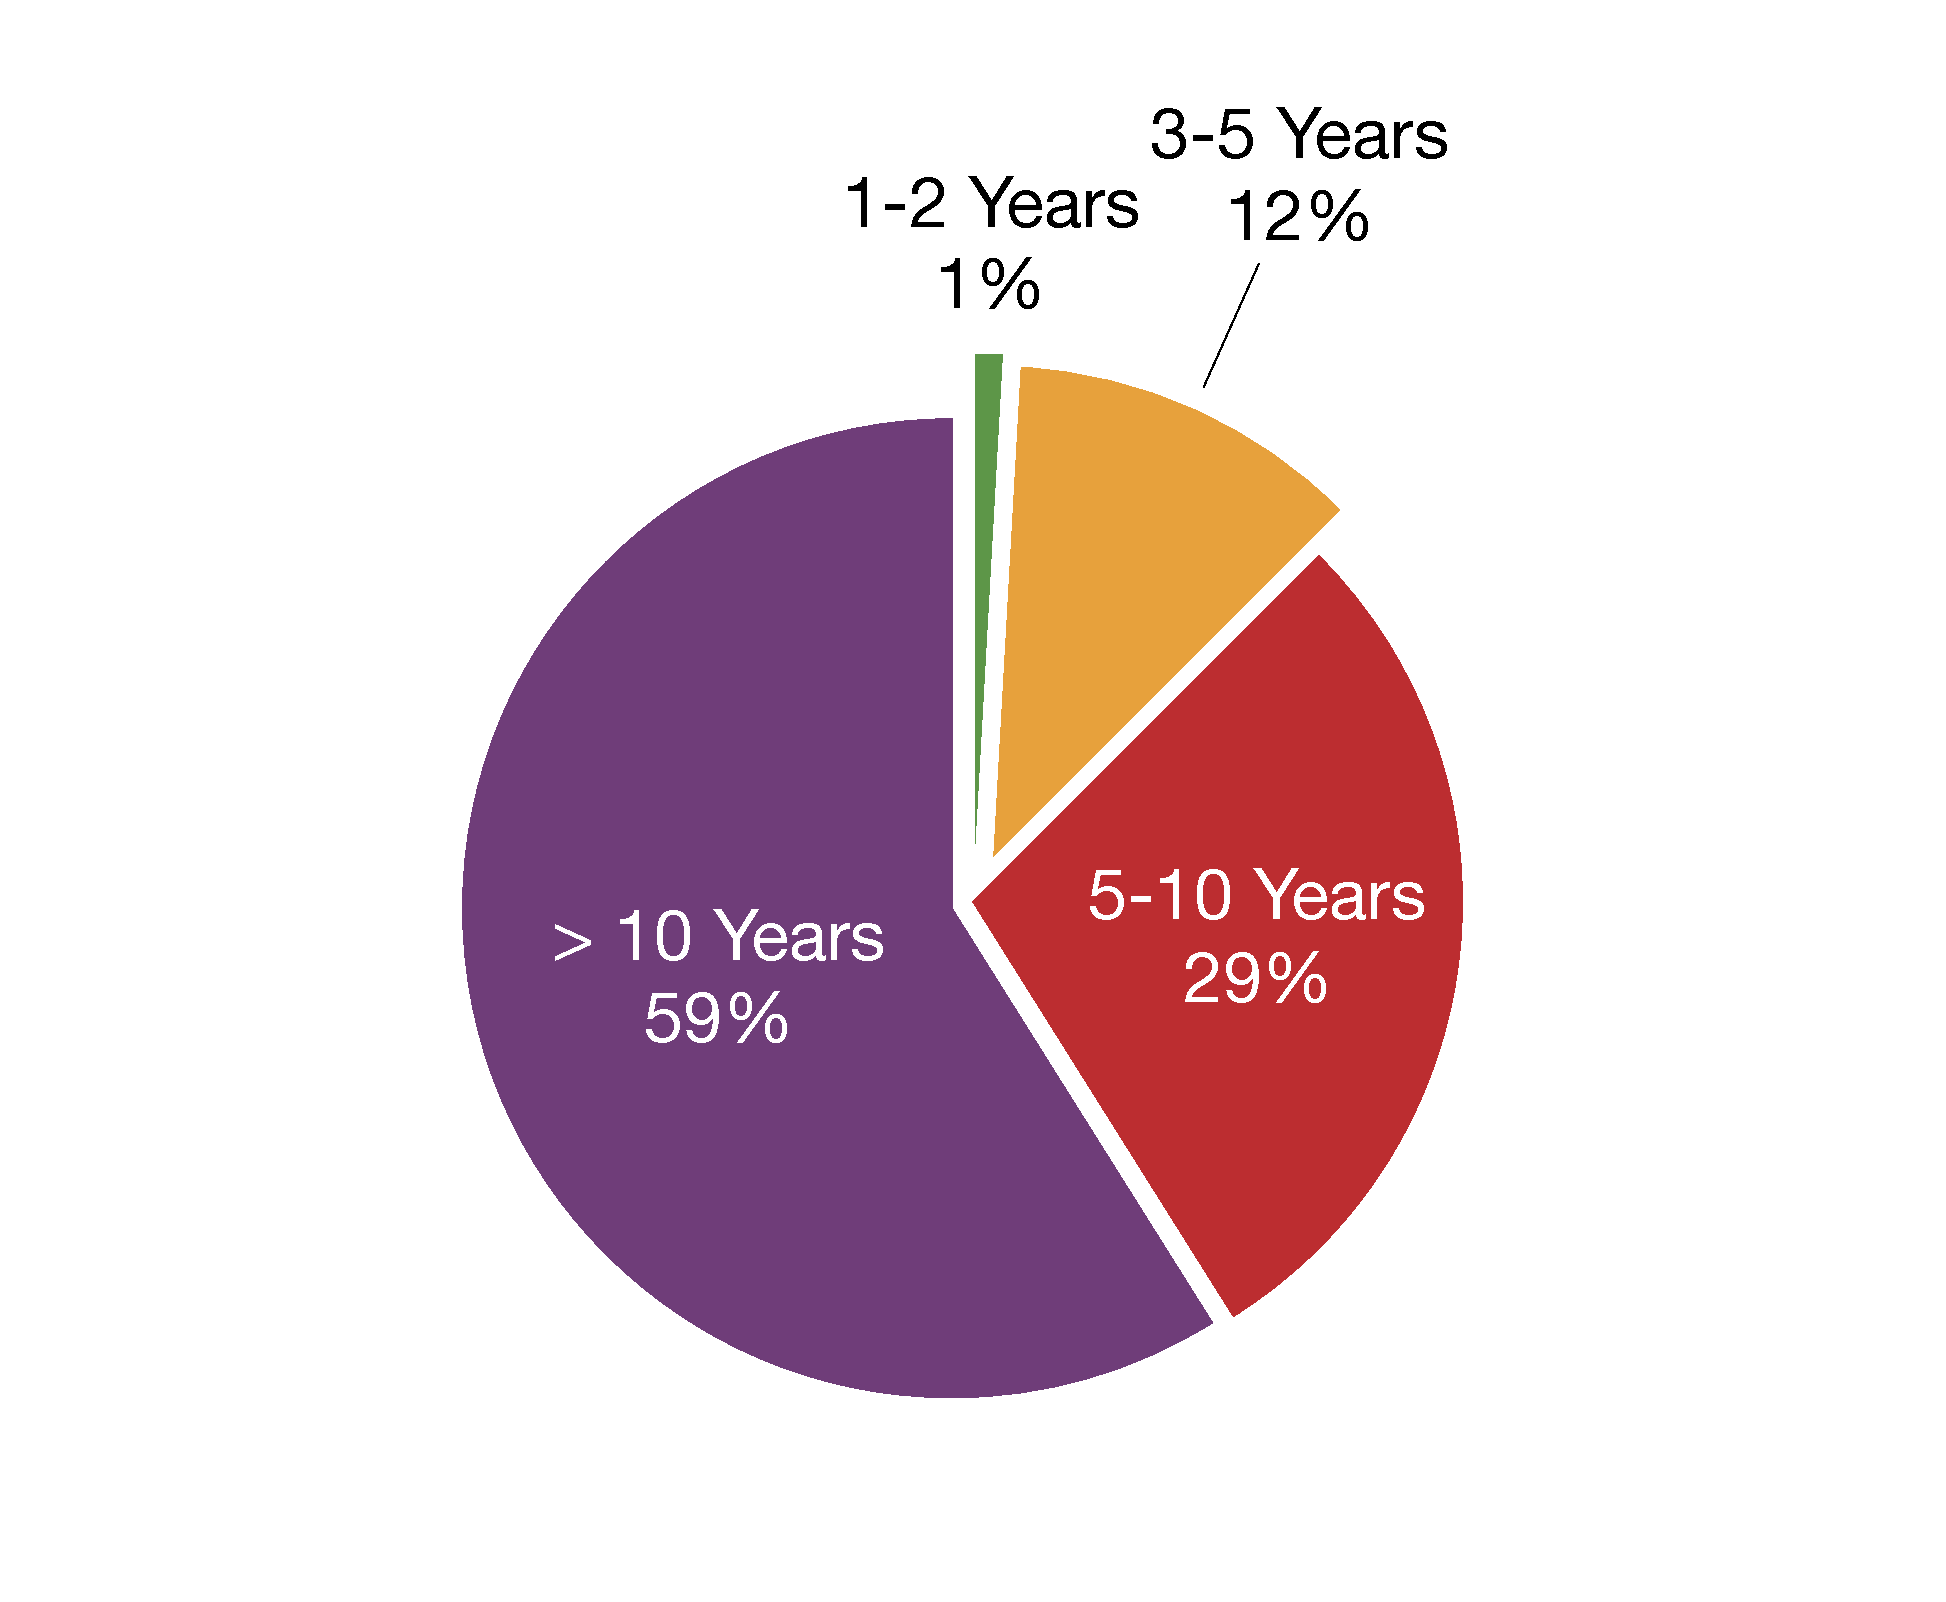
\includegraphics[width=.6\linewidth]{survey_exp_1-crop}
		\caption{Group 1}
		\label{fig:survey_group1_exp}
	\end{subfigure}%
	\begin{subfigure}{.25\textwidth}
		\centering
		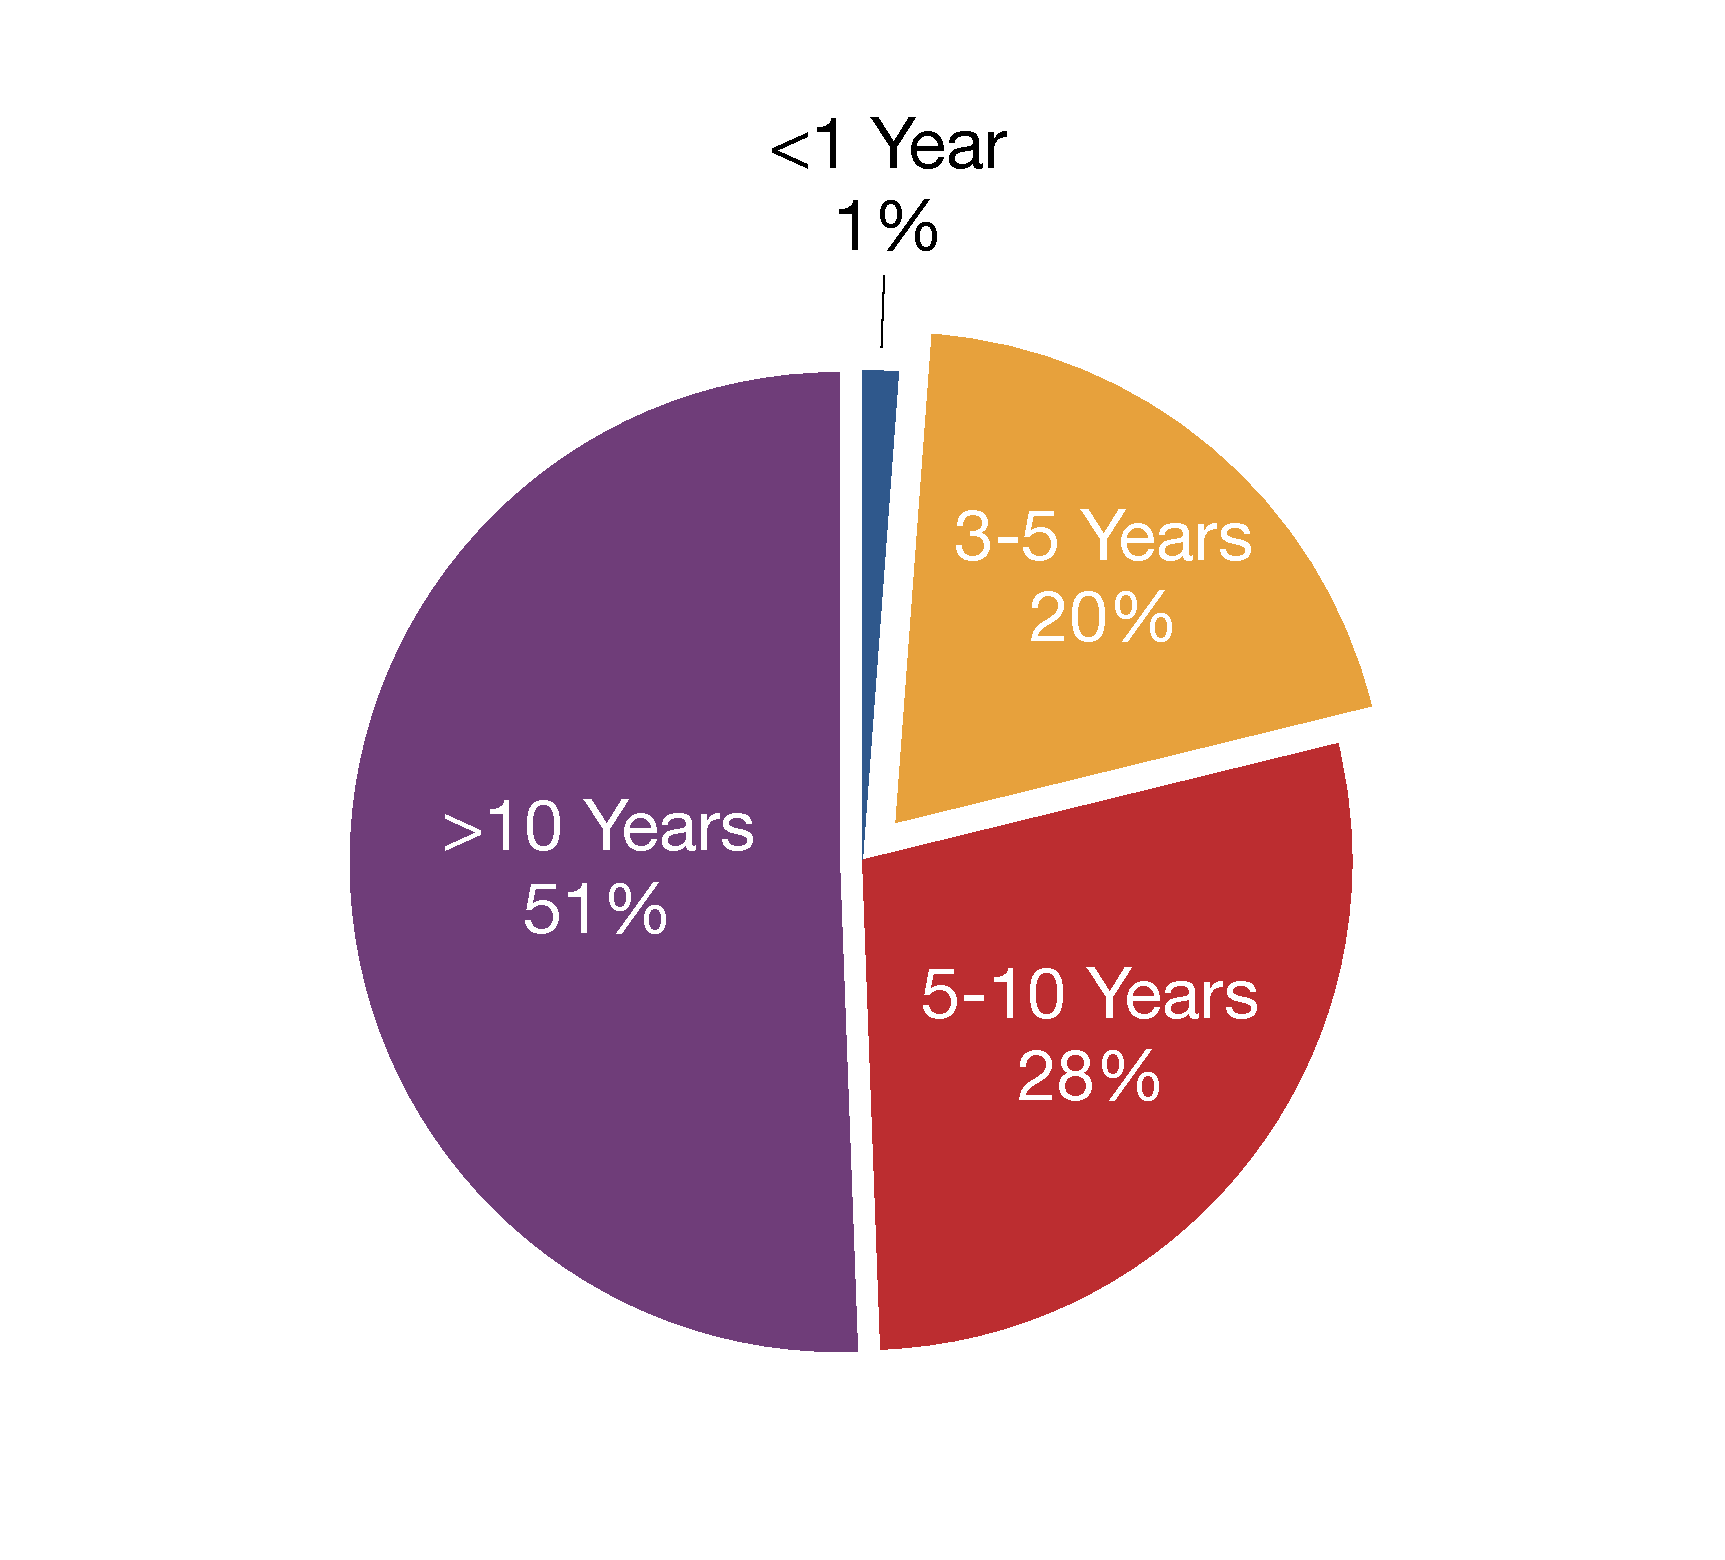
\includegraphics[width=.62\linewidth]{survey_exp_2-crop}
		\caption{Group 2}
		\label{fig:survey_group2_exp}
	\end{subfigure}
	\caption{Experience of the Stack Overflow users}
	\label{fig:survey_exp}
\end{figure}

\subsubsection{Answerers' Experience}
The majority of users in both groups are experienced developers 
with more than 10 years of experience or between 5 to 10 years 
as depicted in \Cref{fig:survey_exp}. They are active users and
regularly answer questions on Stack Overflow.
Eighty one and sixty percent of users from Group 1 and Group 2 
answer questions at least once a week.

\begin{figure*}
	\begin{subfigure}{.5\textwidth}
		\centering
		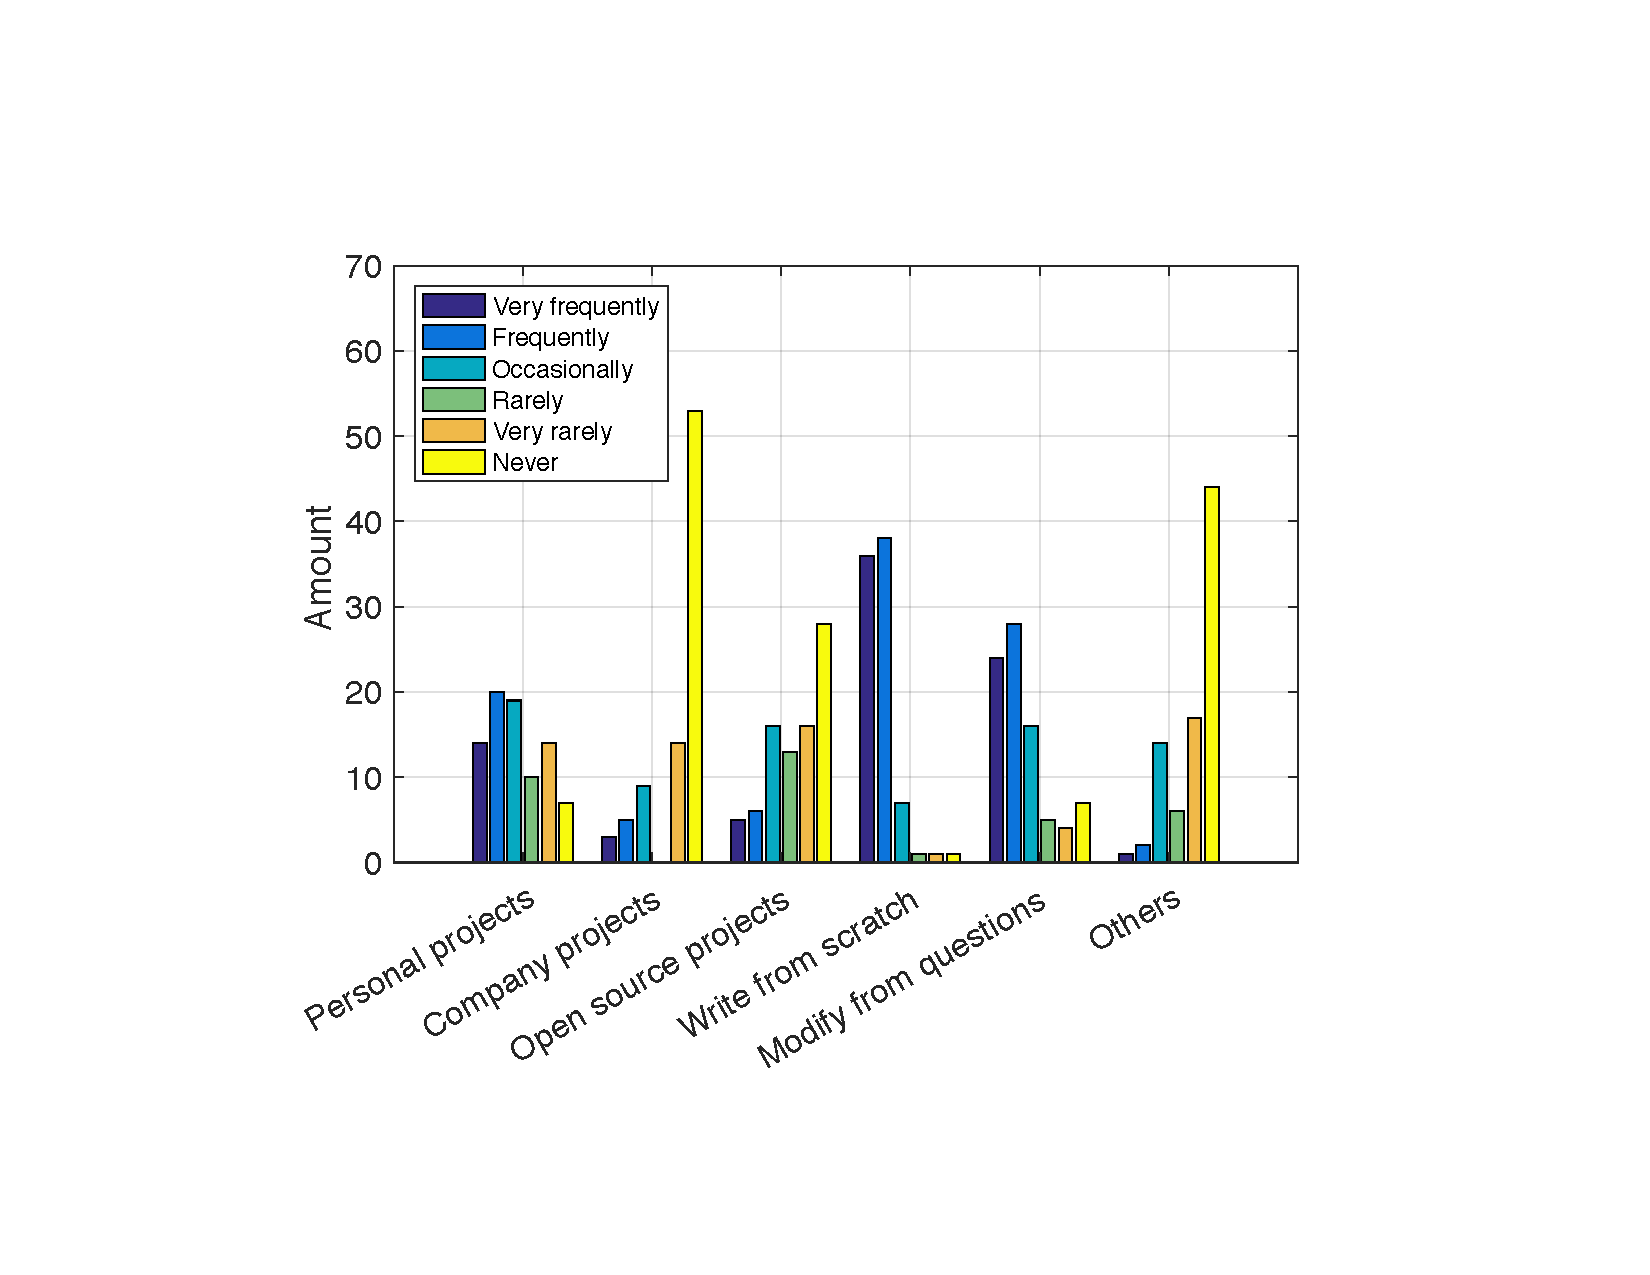
\includegraphics[width=.8\linewidth]{survey_snippet_source_1}
		\caption{Group 1}
		\label{fig:survey_snippet_source_1}
	\end{subfigure}%
	\begin{subfigure}{.5\textwidth}
		\centering
		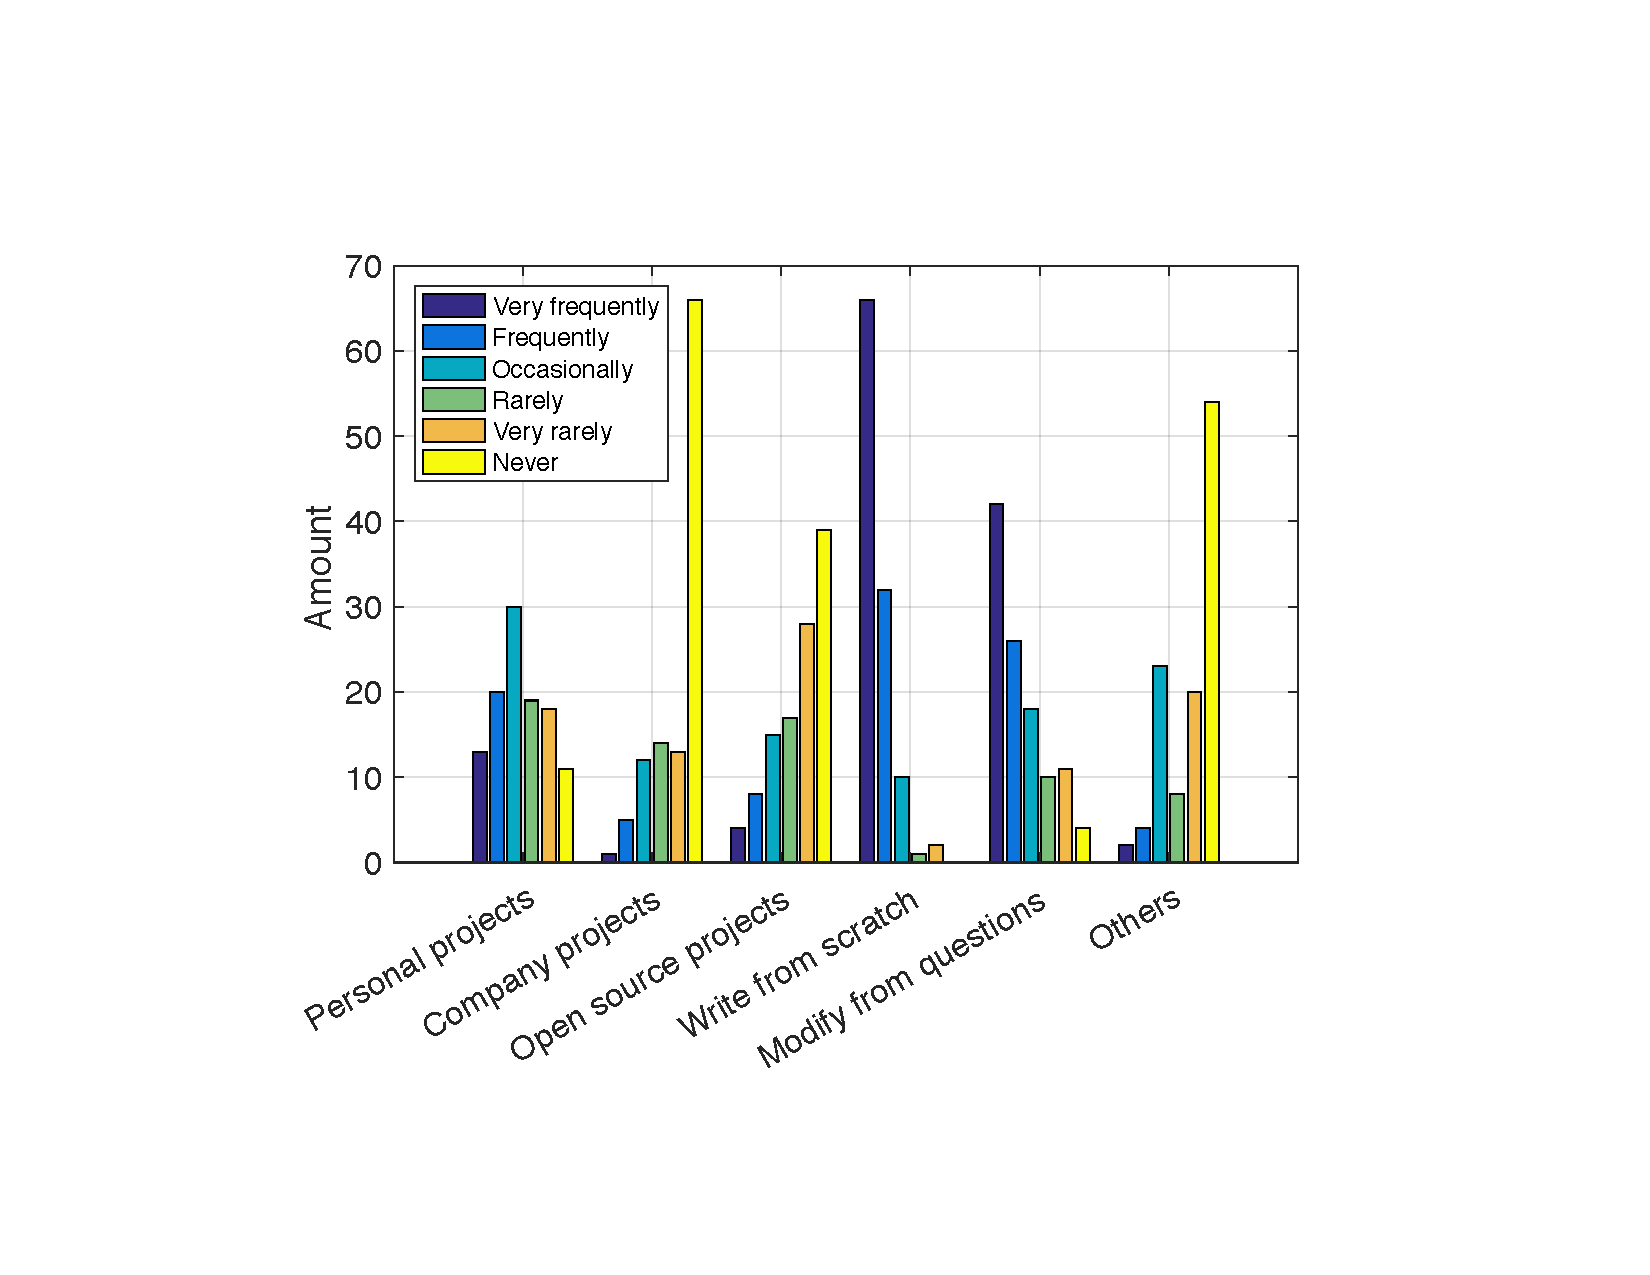
\includegraphics[width=.8\linewidth]{survey_snippet_source_2}
		\caption{Group 2}
		\label{fig:survey_snippet_source_2}
	\end{subfigure}
	\caption{Sources of code snippets in Stack Overflow answers}
	\label{fig:survey_snippet_source}
\end{figure*}

\subsubsection{Code Snippets in Answers} 
A large amount of 91 (81\%) and 58
(68\%) users in both group include code snippets in more than sixty percent of
their answers. \Cref{fig:survey_snippet_source} explains where are these code
snippets from. Stack Overflow answerers mostly write new code from scratch 
or modify from the code snippets in question for each answer, while 
fewer numbers are from other sources including their personal projects, 
their company projects, open source projects. We found 27 answerers in both Group 1
and Group 2 occasionally to very frequently copy code from open source projects.

\begin{figure}
	\begin{subfigure}{.25\textwidth}
		\centering
		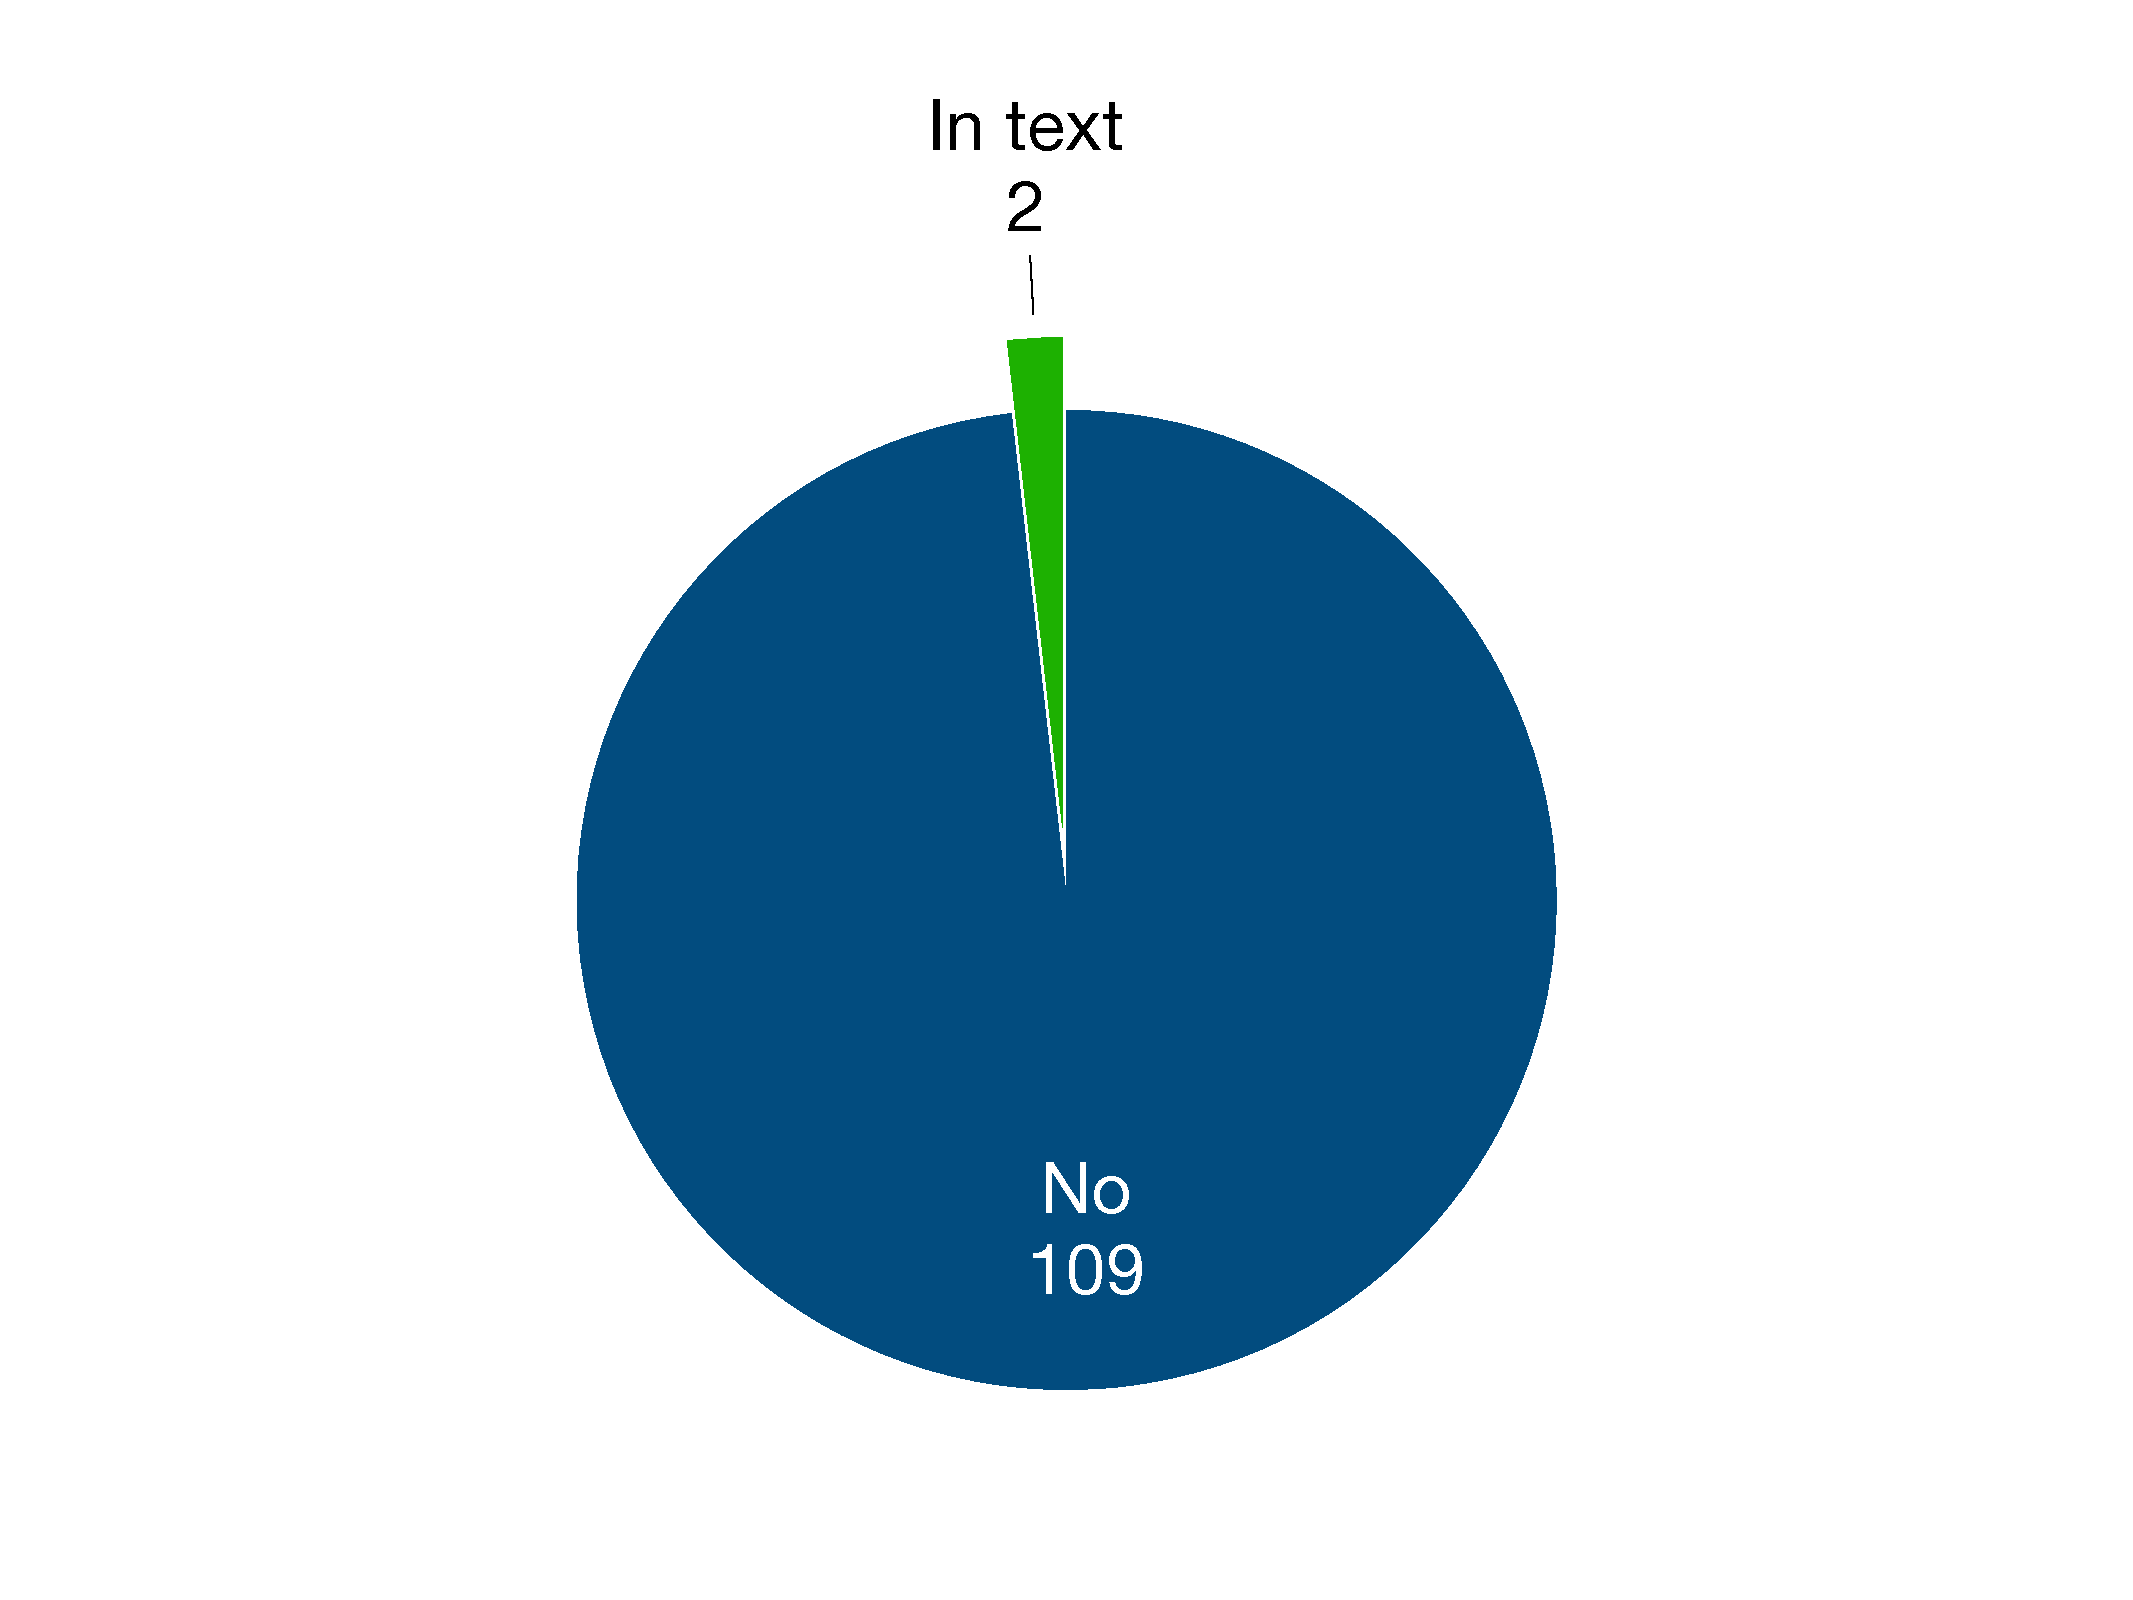
\includegraphics[width=.6\linewidth]{survey_license_1}
		\caption{Group 1}
		\label{fig:survey_license_1}
	\end{subfigure}%
	\begin{subfigure}{.25\textwidth}
		\centering
		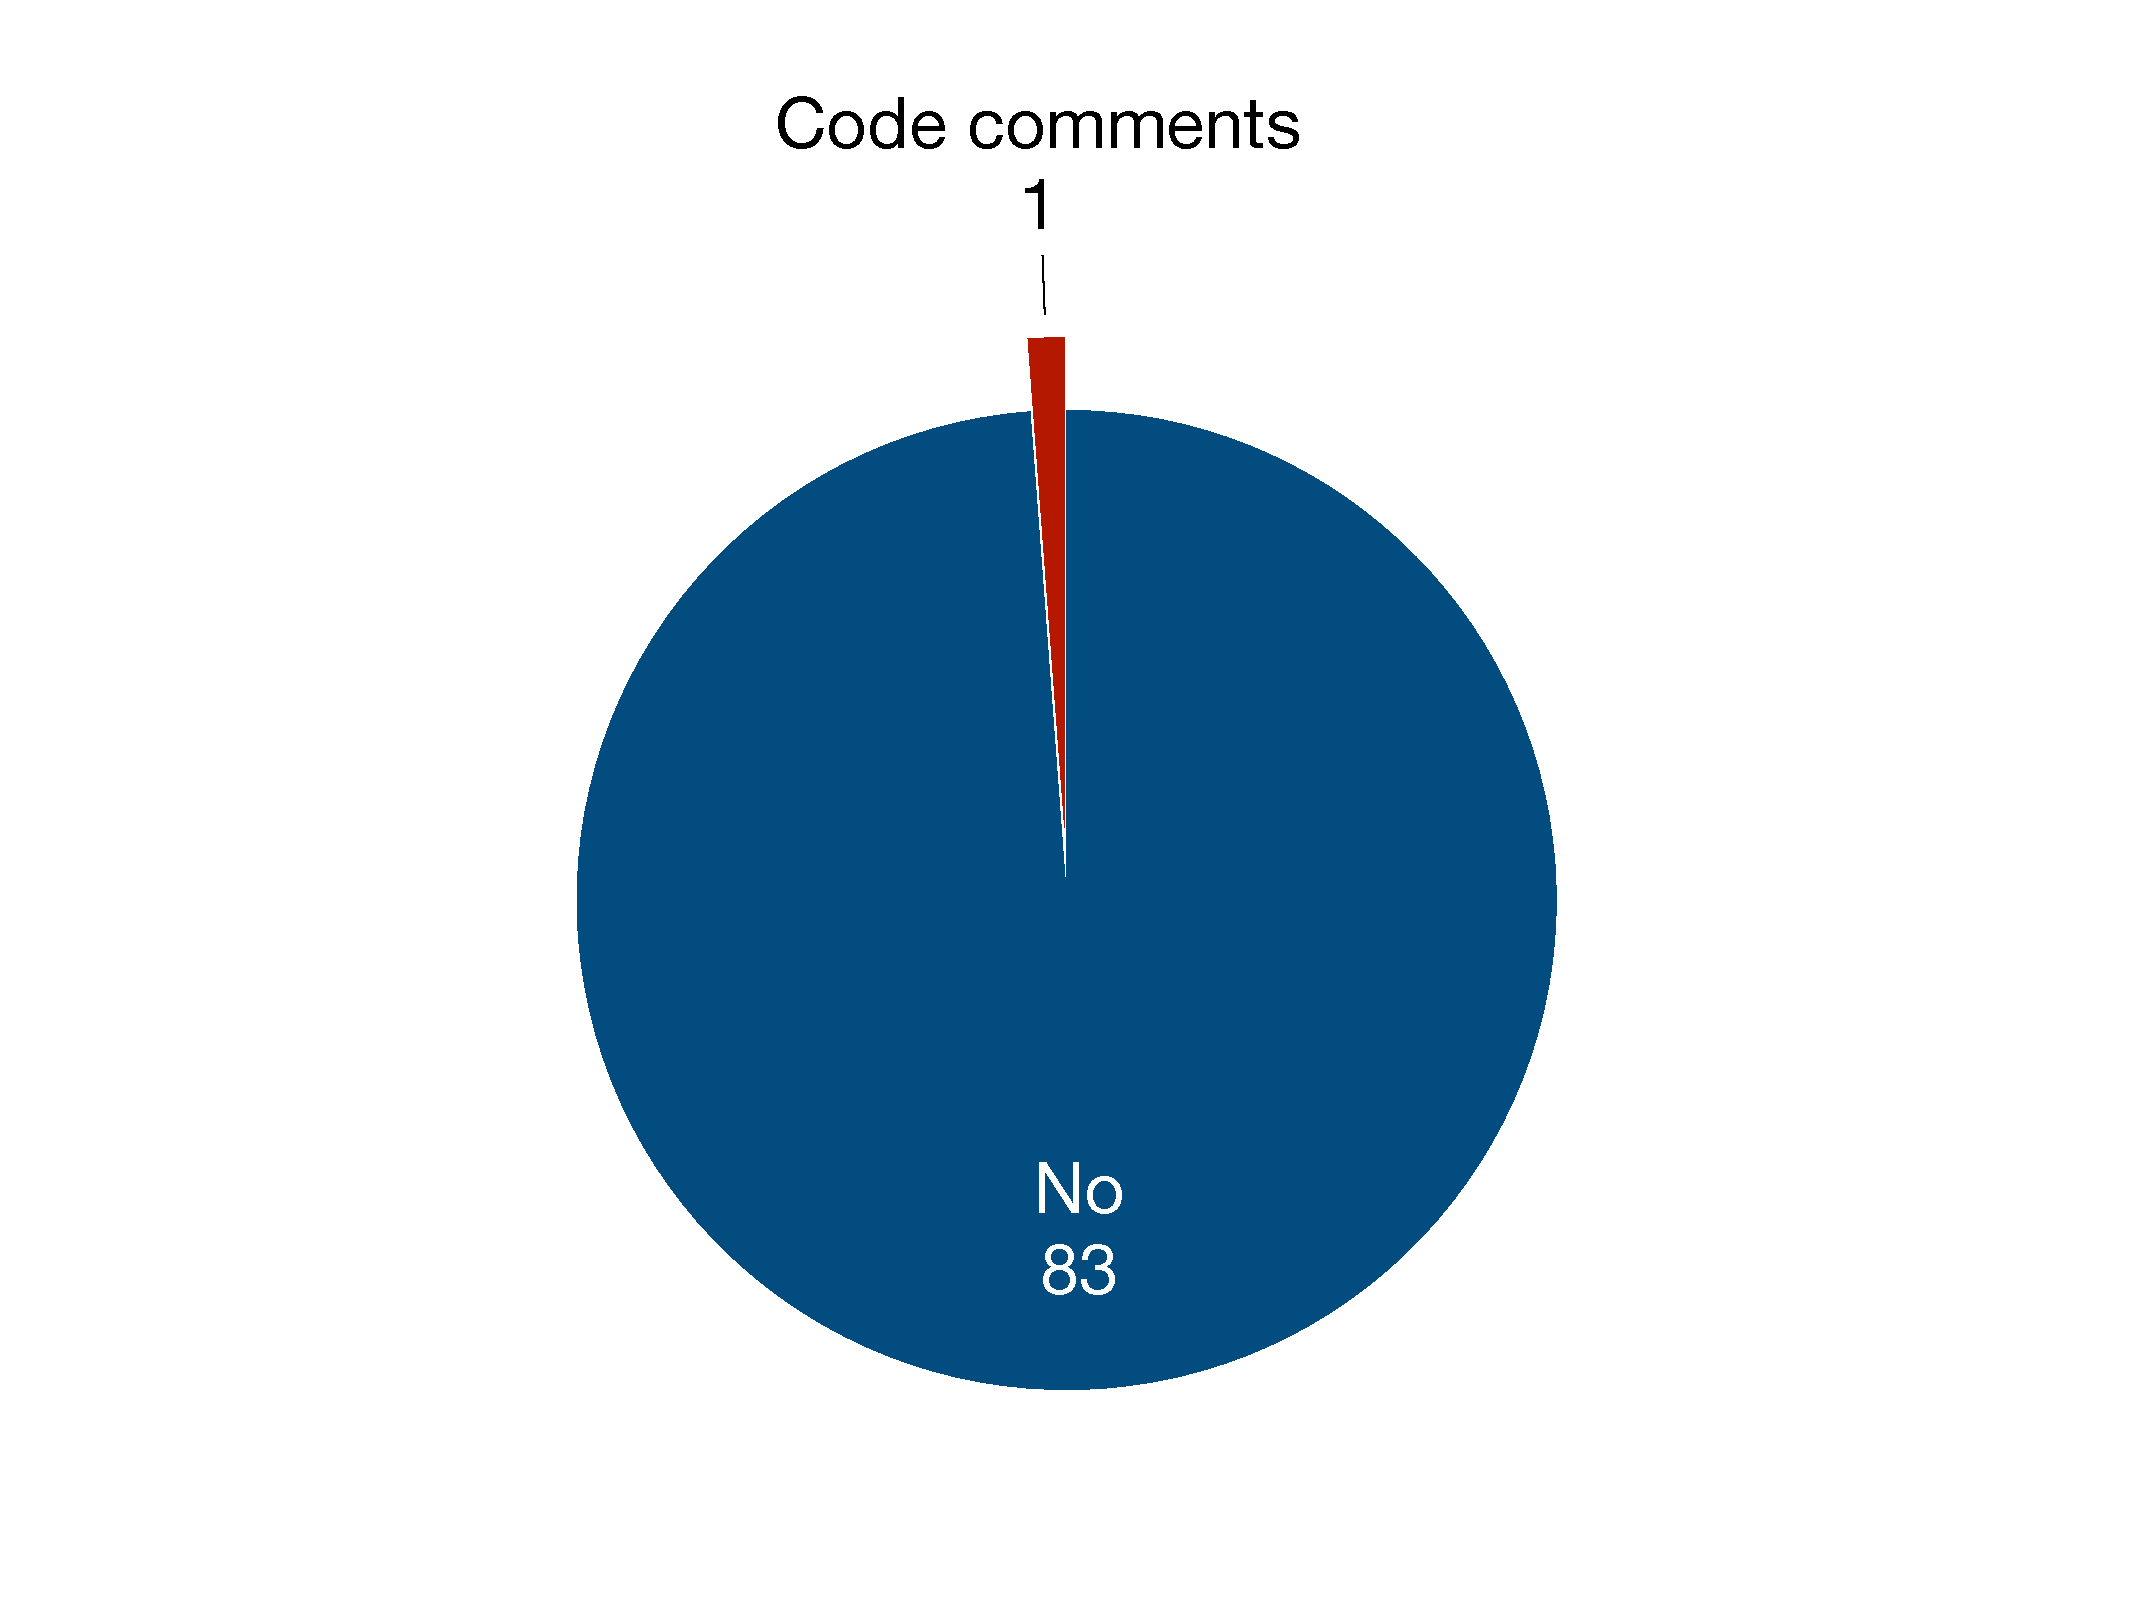
\includegraphics[width=.6\linewidth]{survey_license_2}
		\caption{Group 2}
		\label{fig:survey_license_2}
	\end{subfigure}
	\caption{Software license in Stack Overflow code snippets.}
	\label{fig:survey_license}
\end{figure}

\subsubsection{Outdated Code Snippets} 

We found that 63.1\% of Stack Overflow answerers in Group 1 have been notified of
outdated code in their answers (see \Cref{fig:survey_outdated}). The ratio drops to 47.6\% in
Group 2. Thus, at least roughly half of the top answerers on Stack Overflow
are aware of their outdated code in some of their answers.

\begin{figure}
	\centering
	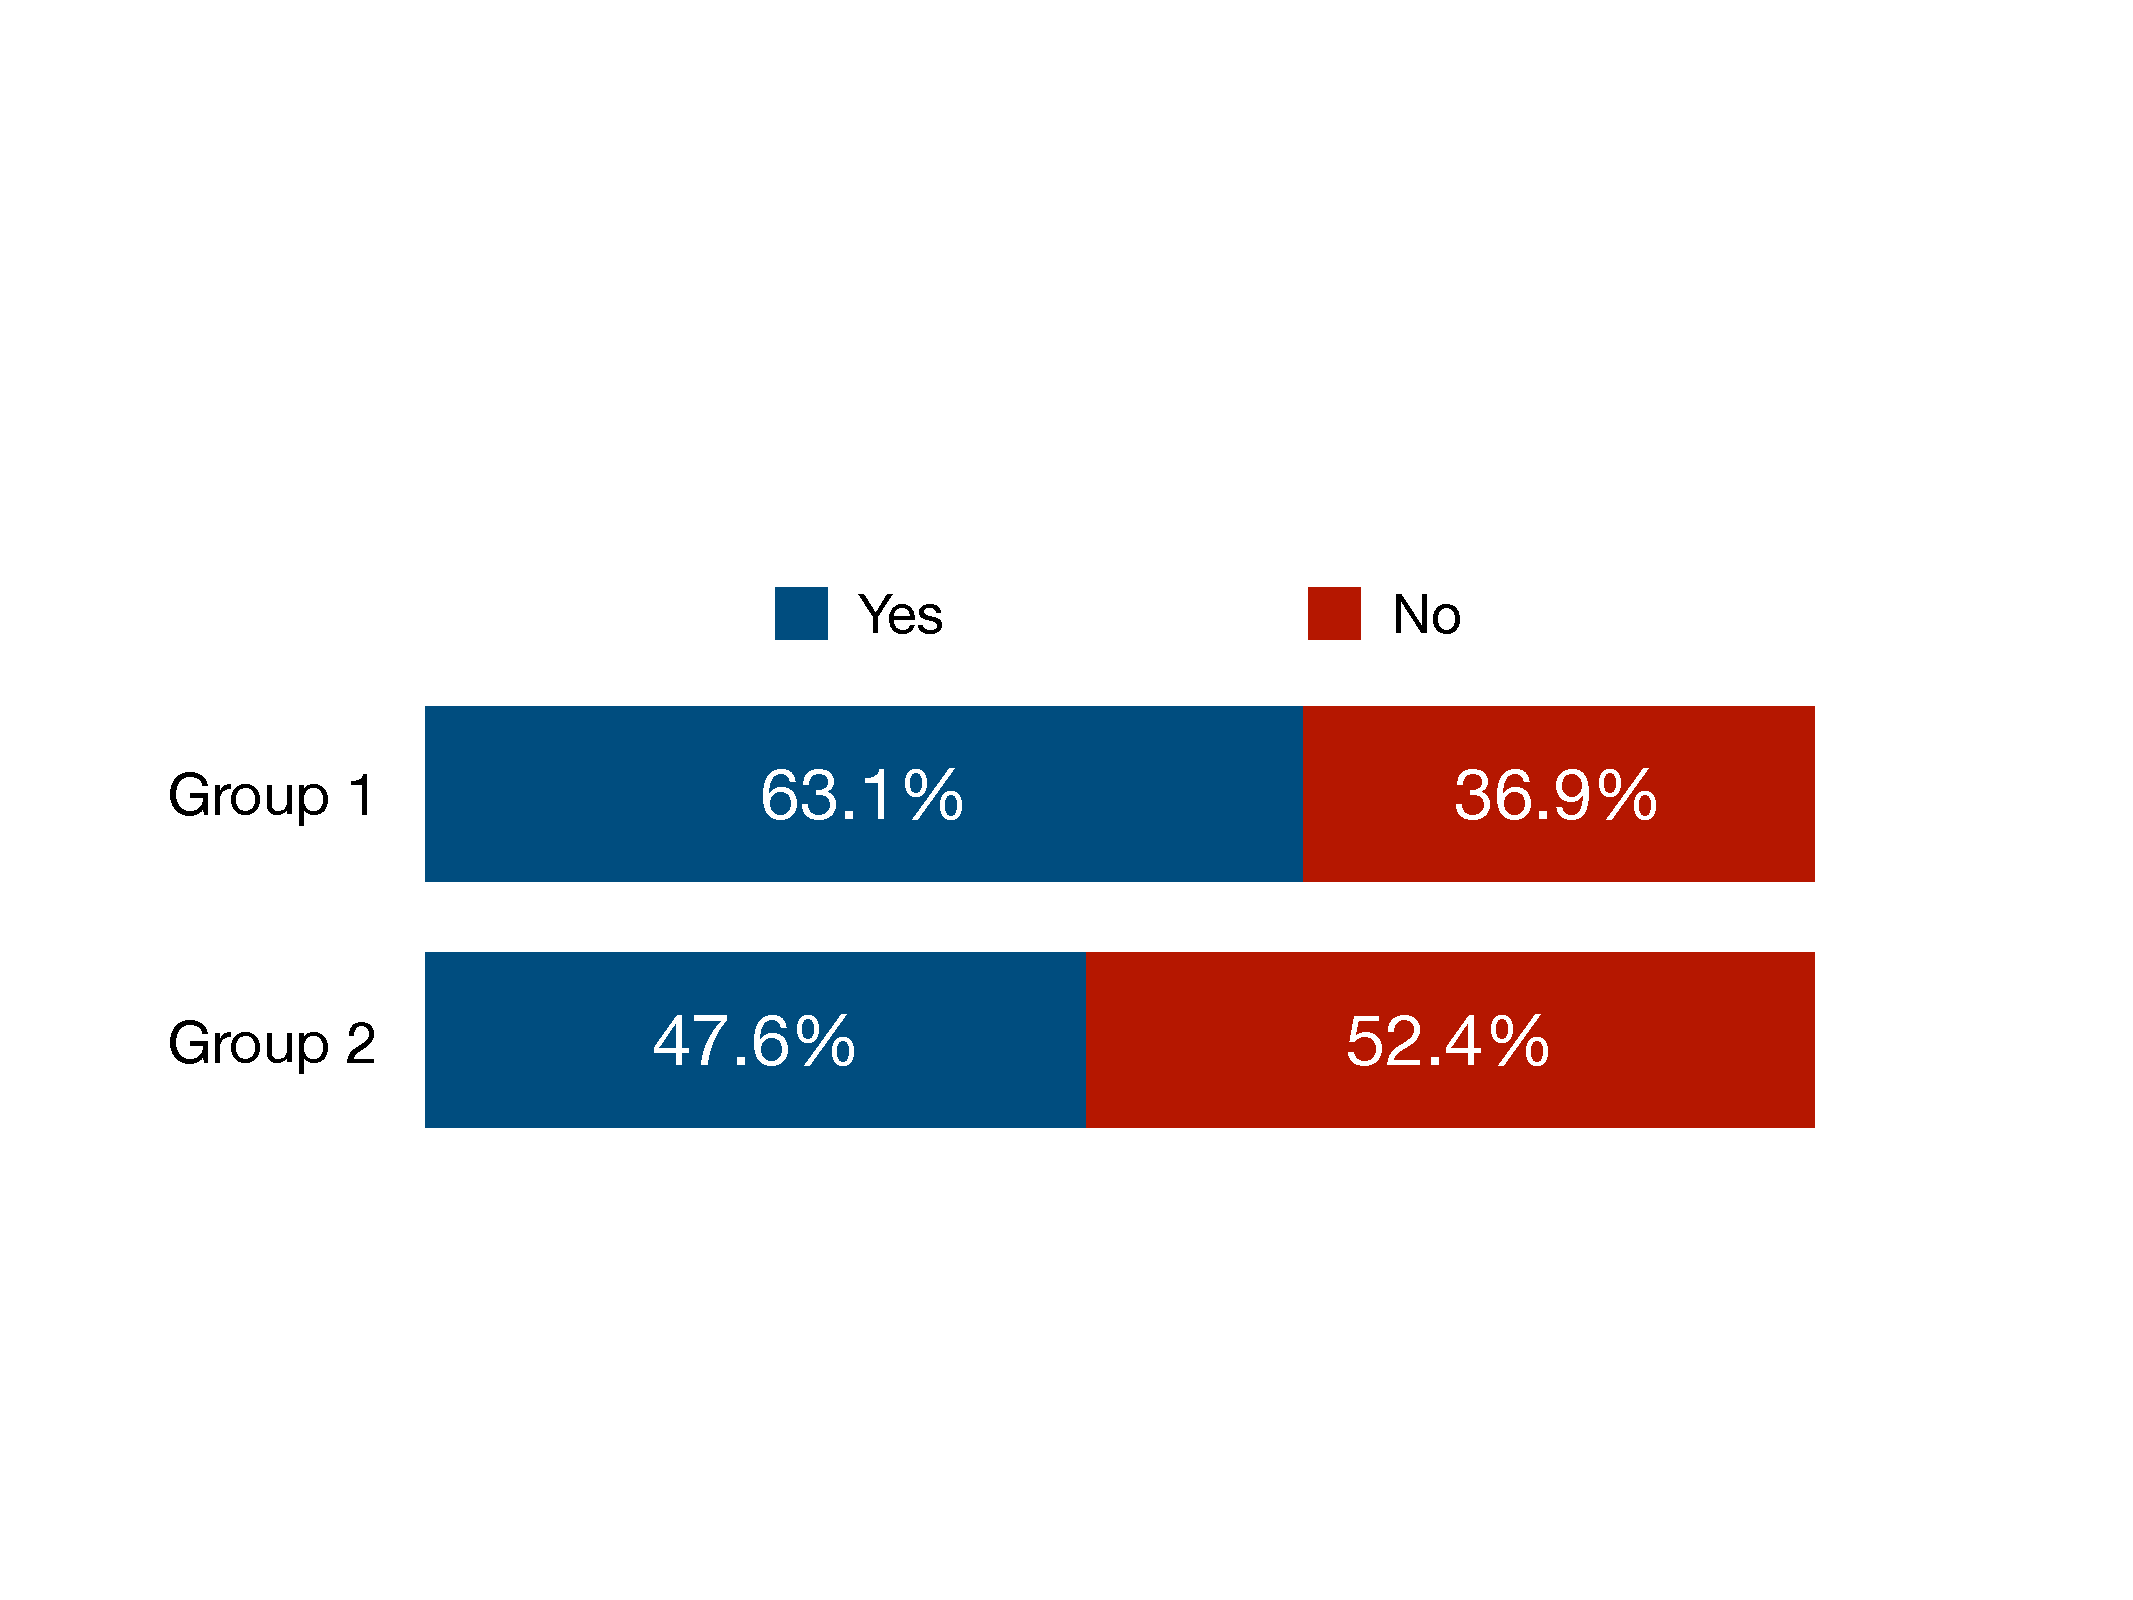
\includegraphics[width=.8\linewidth]{survey_outdated}
	\caption{Percentage of answerers who are notified of outdated code in their Stack Overflow answers.}
	\label{fig:survey_outdated}
\end{figure}%

We then asked the participants to have been notified of their outdated code
(80 and 48 participants from Group 1 and 2 respectively) a
follow-up questions ``how frequently did you fix your outdated code on Stack
Overflow?''. The answers, depicted in \Cref{fig:survey_outdated_fix}, show that
more than half of them frequently fix the outdated code snippets. However, there
are 18.8\% of the answerers in both groups who rarely or never fix their code.

\begin{figure}
	\begin{subfigure}{.25\textwidth}
		\centering
		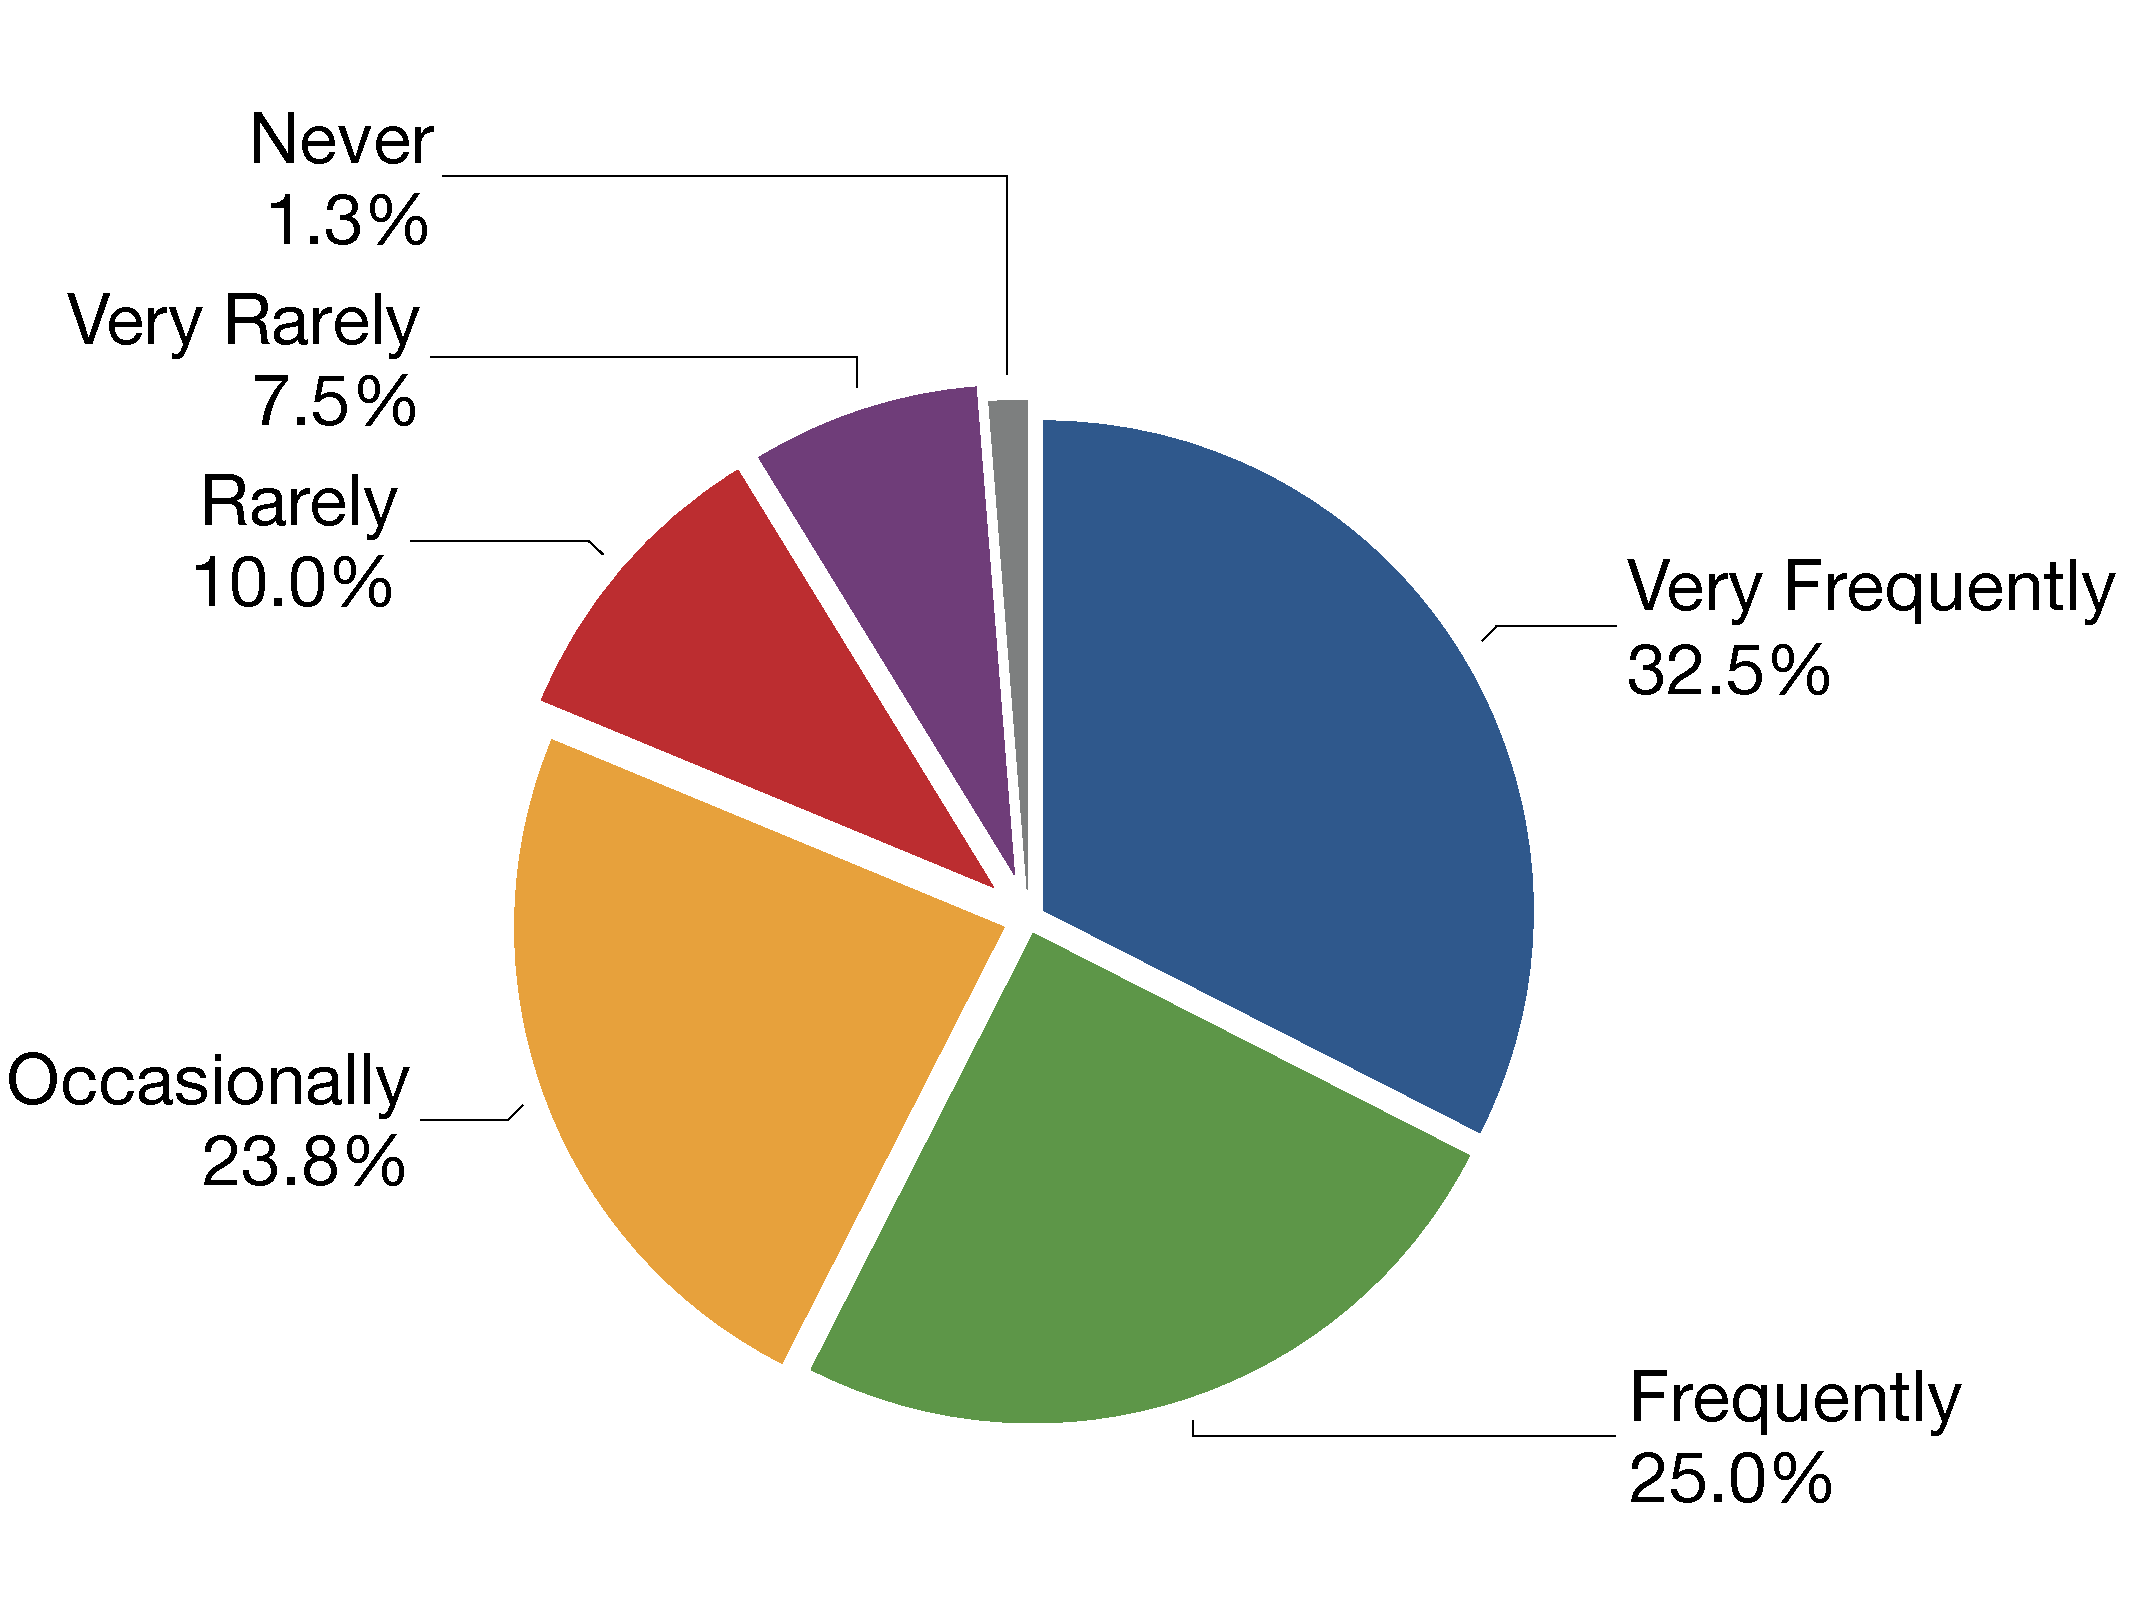
\includegraphics[width=\linewidth]{survey_outdated_fix_1}
		\caption{Group 1}
		\label{fig:survey_outdated_fix_1}
	\end{subfigure}%
	\begin{subfigure}{.25\textwidth}
		\centering
		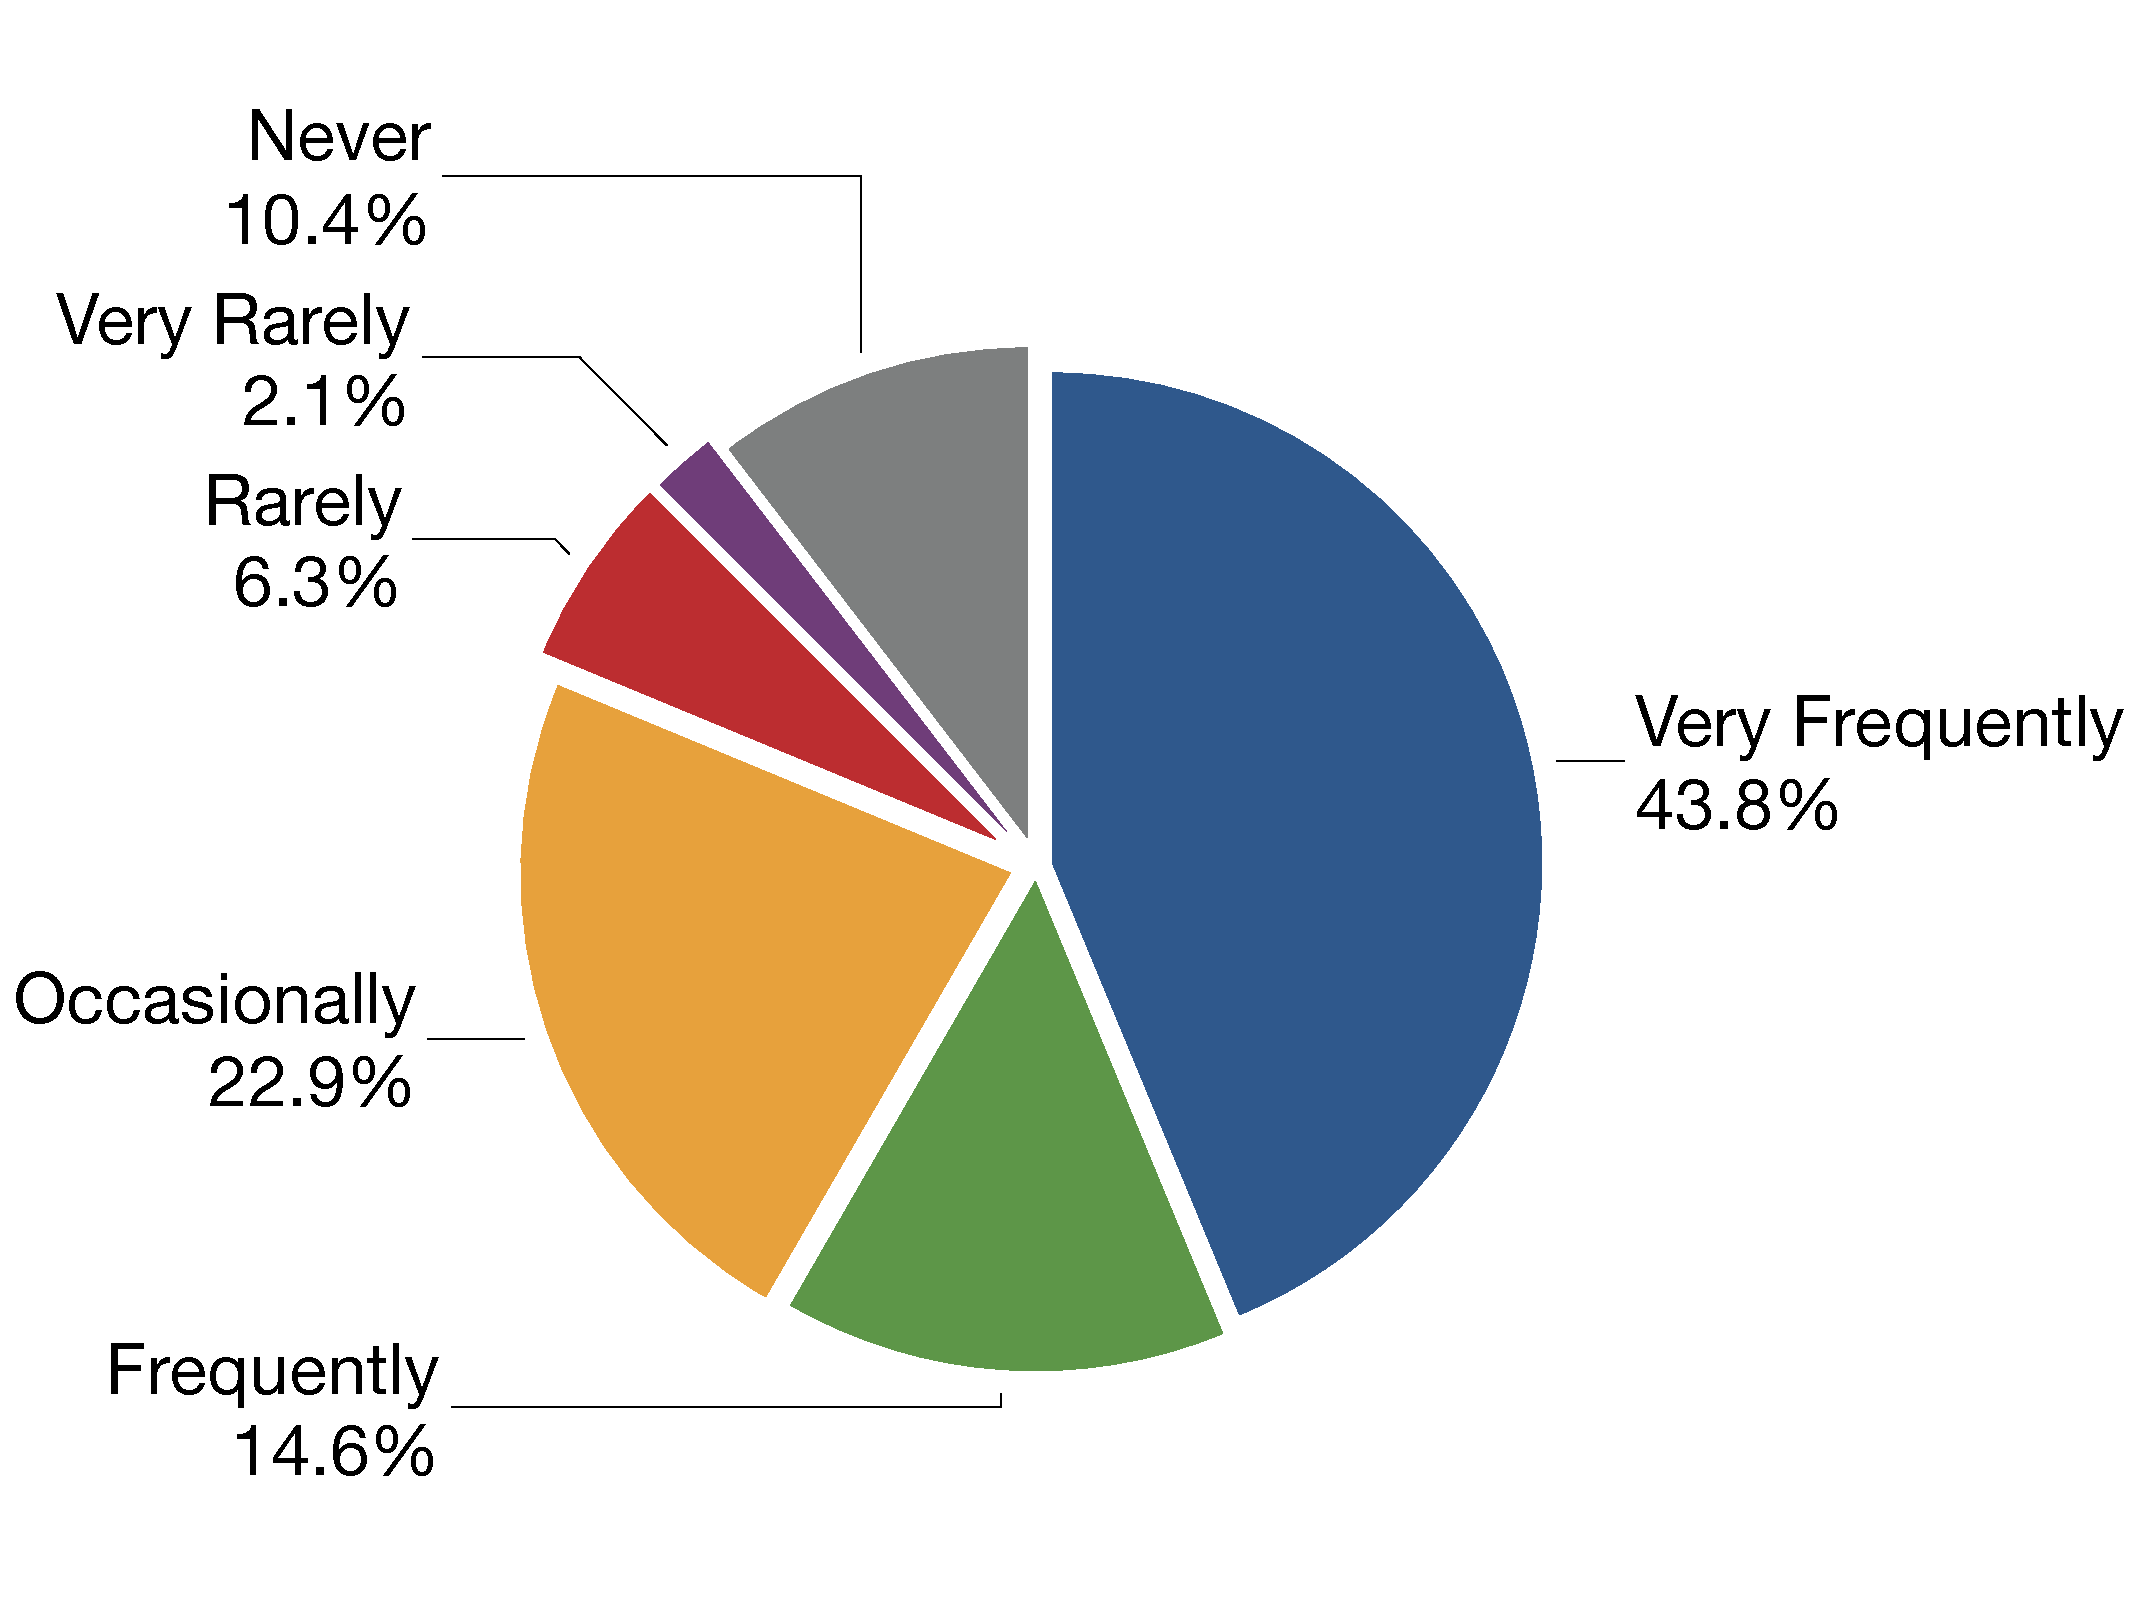
\includegraphics[width=\linewidth]{survey_outdated_fix_2}
		\caption{Group 2}
		\label{fig:survey_outdated_fix_2}
	\end{subfigure}
	\caption{Frequency of the answerers fixing their outdated code.}
	\label{fig:survey_outdated_fix}
\end{figure}

The answers support our findings of outdated online code clones. Although most
of the Stack Overflow answerers know that their code are outdated, the code may
still not be fixed.

\subsubsection{License of Code Snippets} 
More than half of the answerers in both groups (63.1\% and 61.9\% respectively)
are aware that Stack Overflow apply Creative Commons Attribution-ShareAlike 3.0
Unported (CC BY-SA 3.0) to content in the posts, including code snippets, while
the rest of 36.9\% and 38.1\% are not. Nevertheless, we found that almost all 
of them do not include license statement in their code snippets (as depicted in
\Cref{fig:survey_license}) due to several reasons. First, some answerers chose to 
post only their own code or code that was adapted from the question, hence
 they are automatically subjected to CC BY-SA 3.0. Second, they copied code from
company or open source projects that they knew were permitted to be publicly distributed.
Third, some answerers believe that code snippets in their answers are too small 
to claim any intellectual property on them and fall under fair use~\cite{fairuse}.

While nobody explicitly includes a software license in their snippets,
many users include a statement on their profile page that states all their
answers are under a certain license. For example, \textit{All code posted by me on
Stack Overflow should be considered public domain without copyright. For
countries where public domain is not applicable, I hereby grant everyone the
right to modify, use and redistribute any code posted by me on Stack Overflow
for any purpose. It is provided "as-is" without warranty of any kind.}  Many
users either declare their snippets to be public domain, or they grant
additional licenses, e.g. Apache 2.0 or MIT/Expat.

\begin{figure}
	\begin{subfigure}{.25\textwidth}
		\centering
		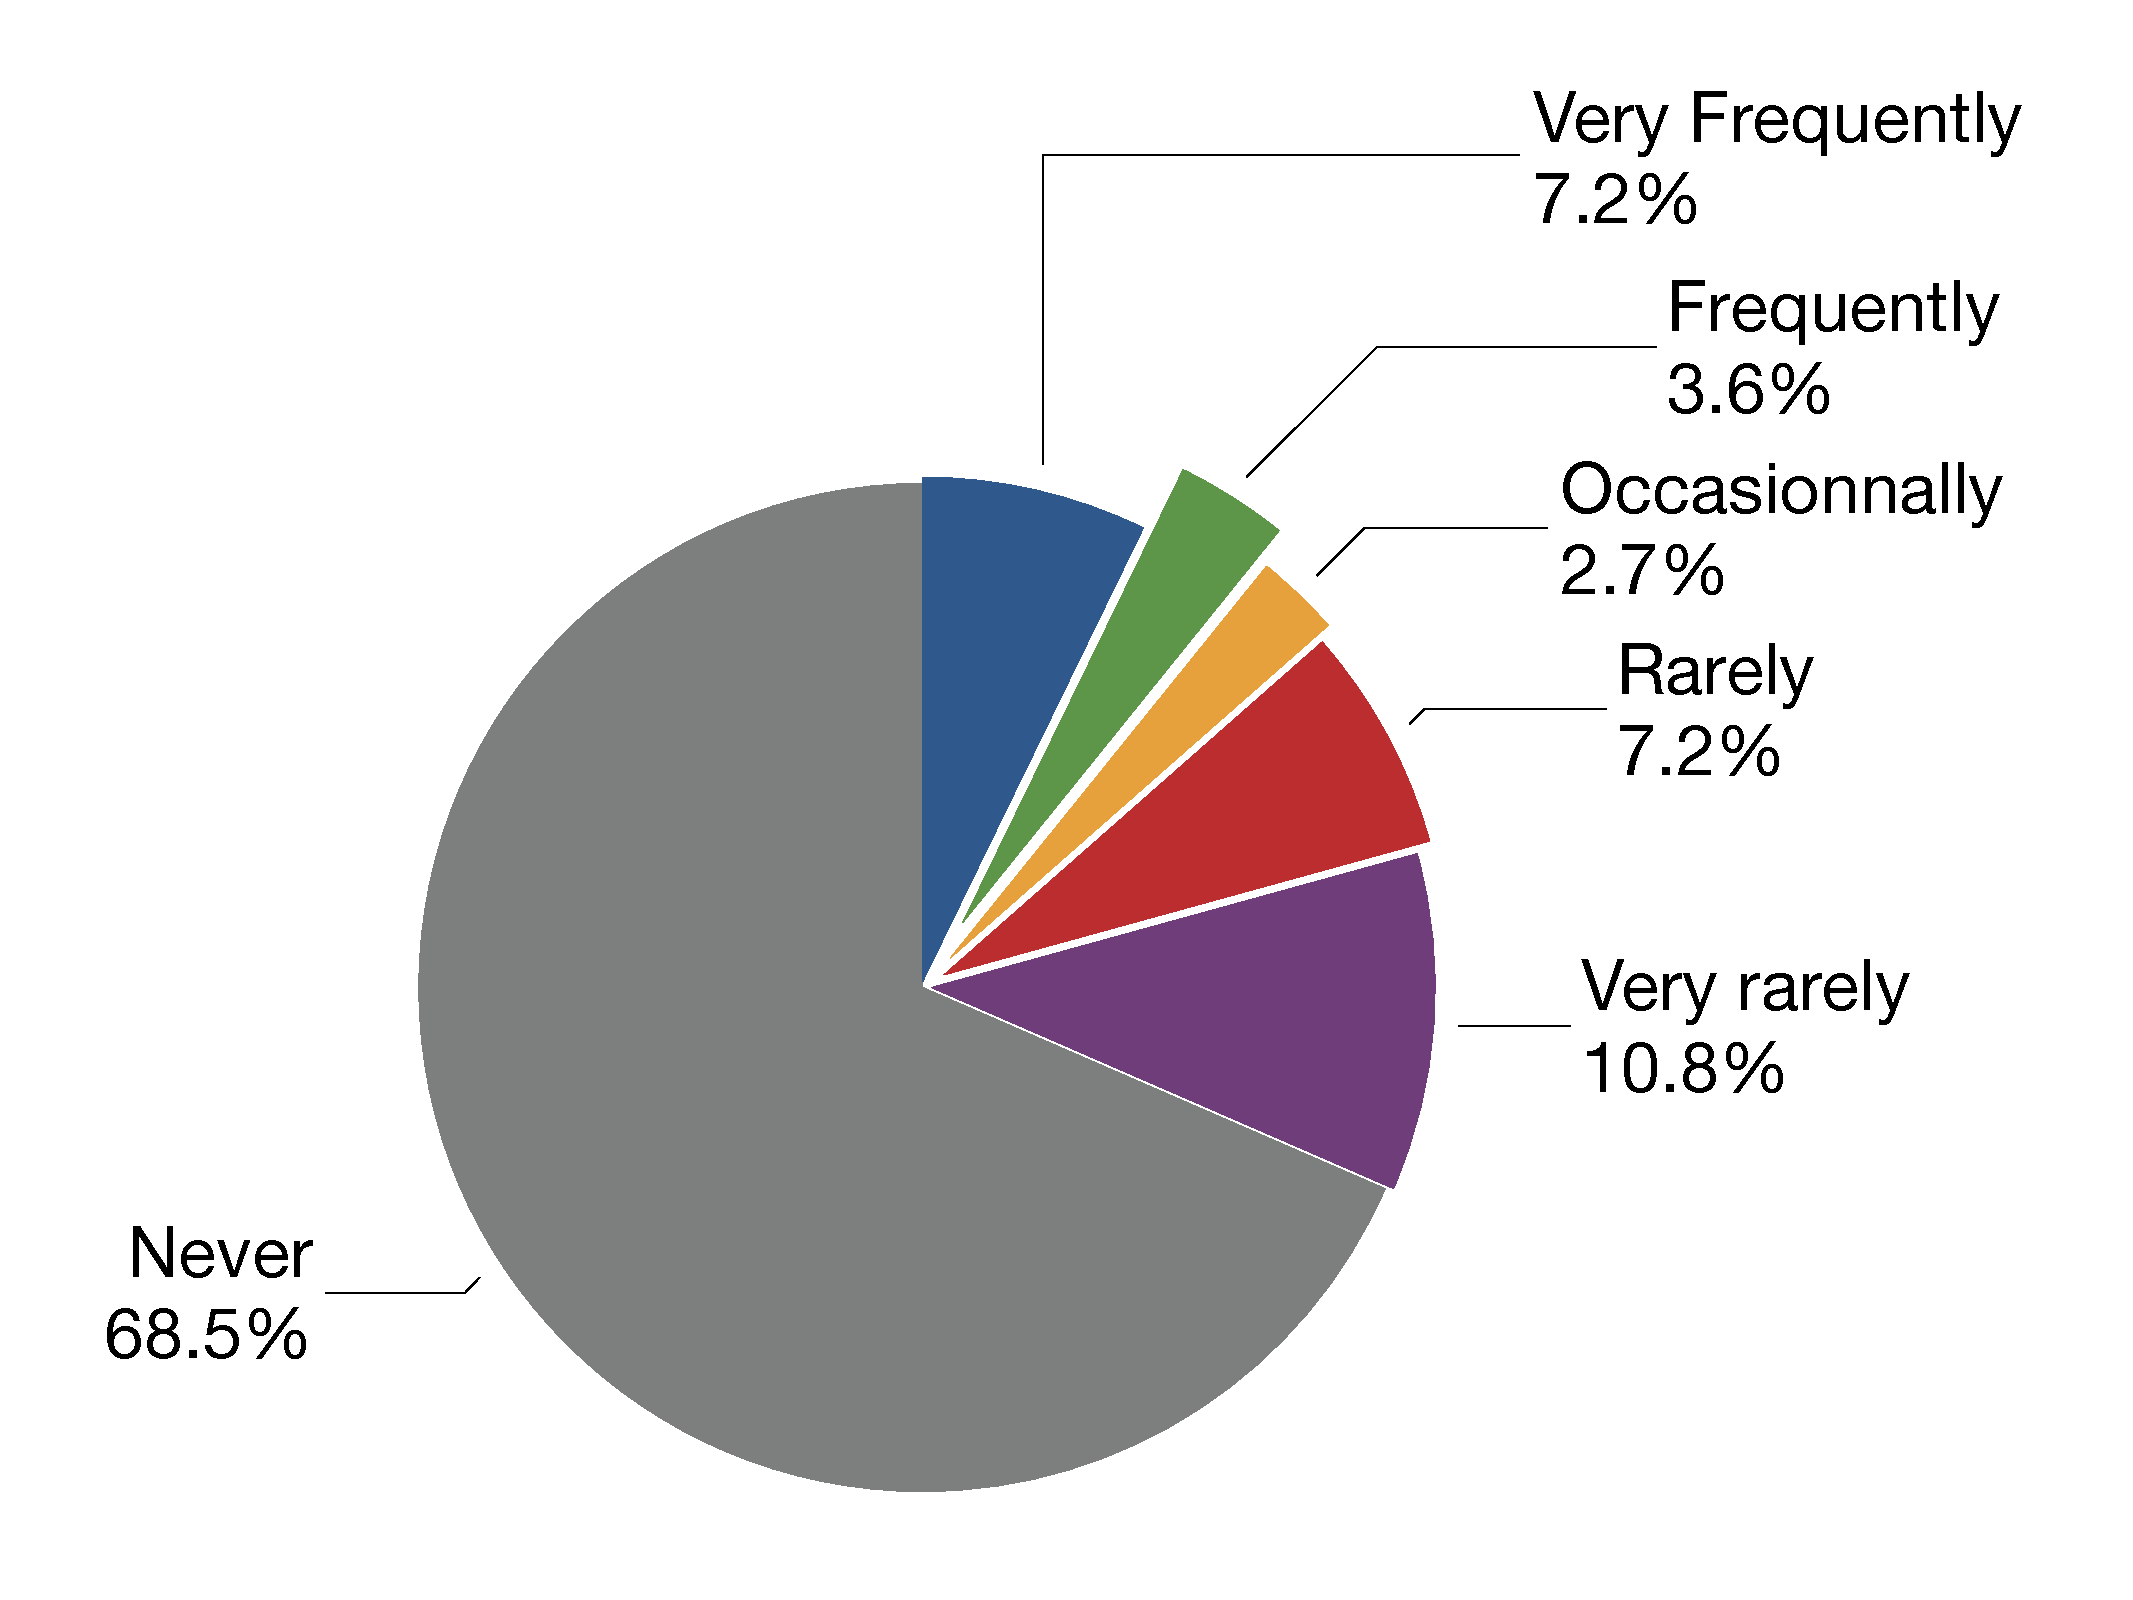
\includegraphics[width=\linewidth]{survey_license_check_1}
		\caption{Group 1}
		\label{fig:survey_license_check_1}
	\end{subfigure}%
	\begin{subfigure}{.25\textwidth}
		\centering
		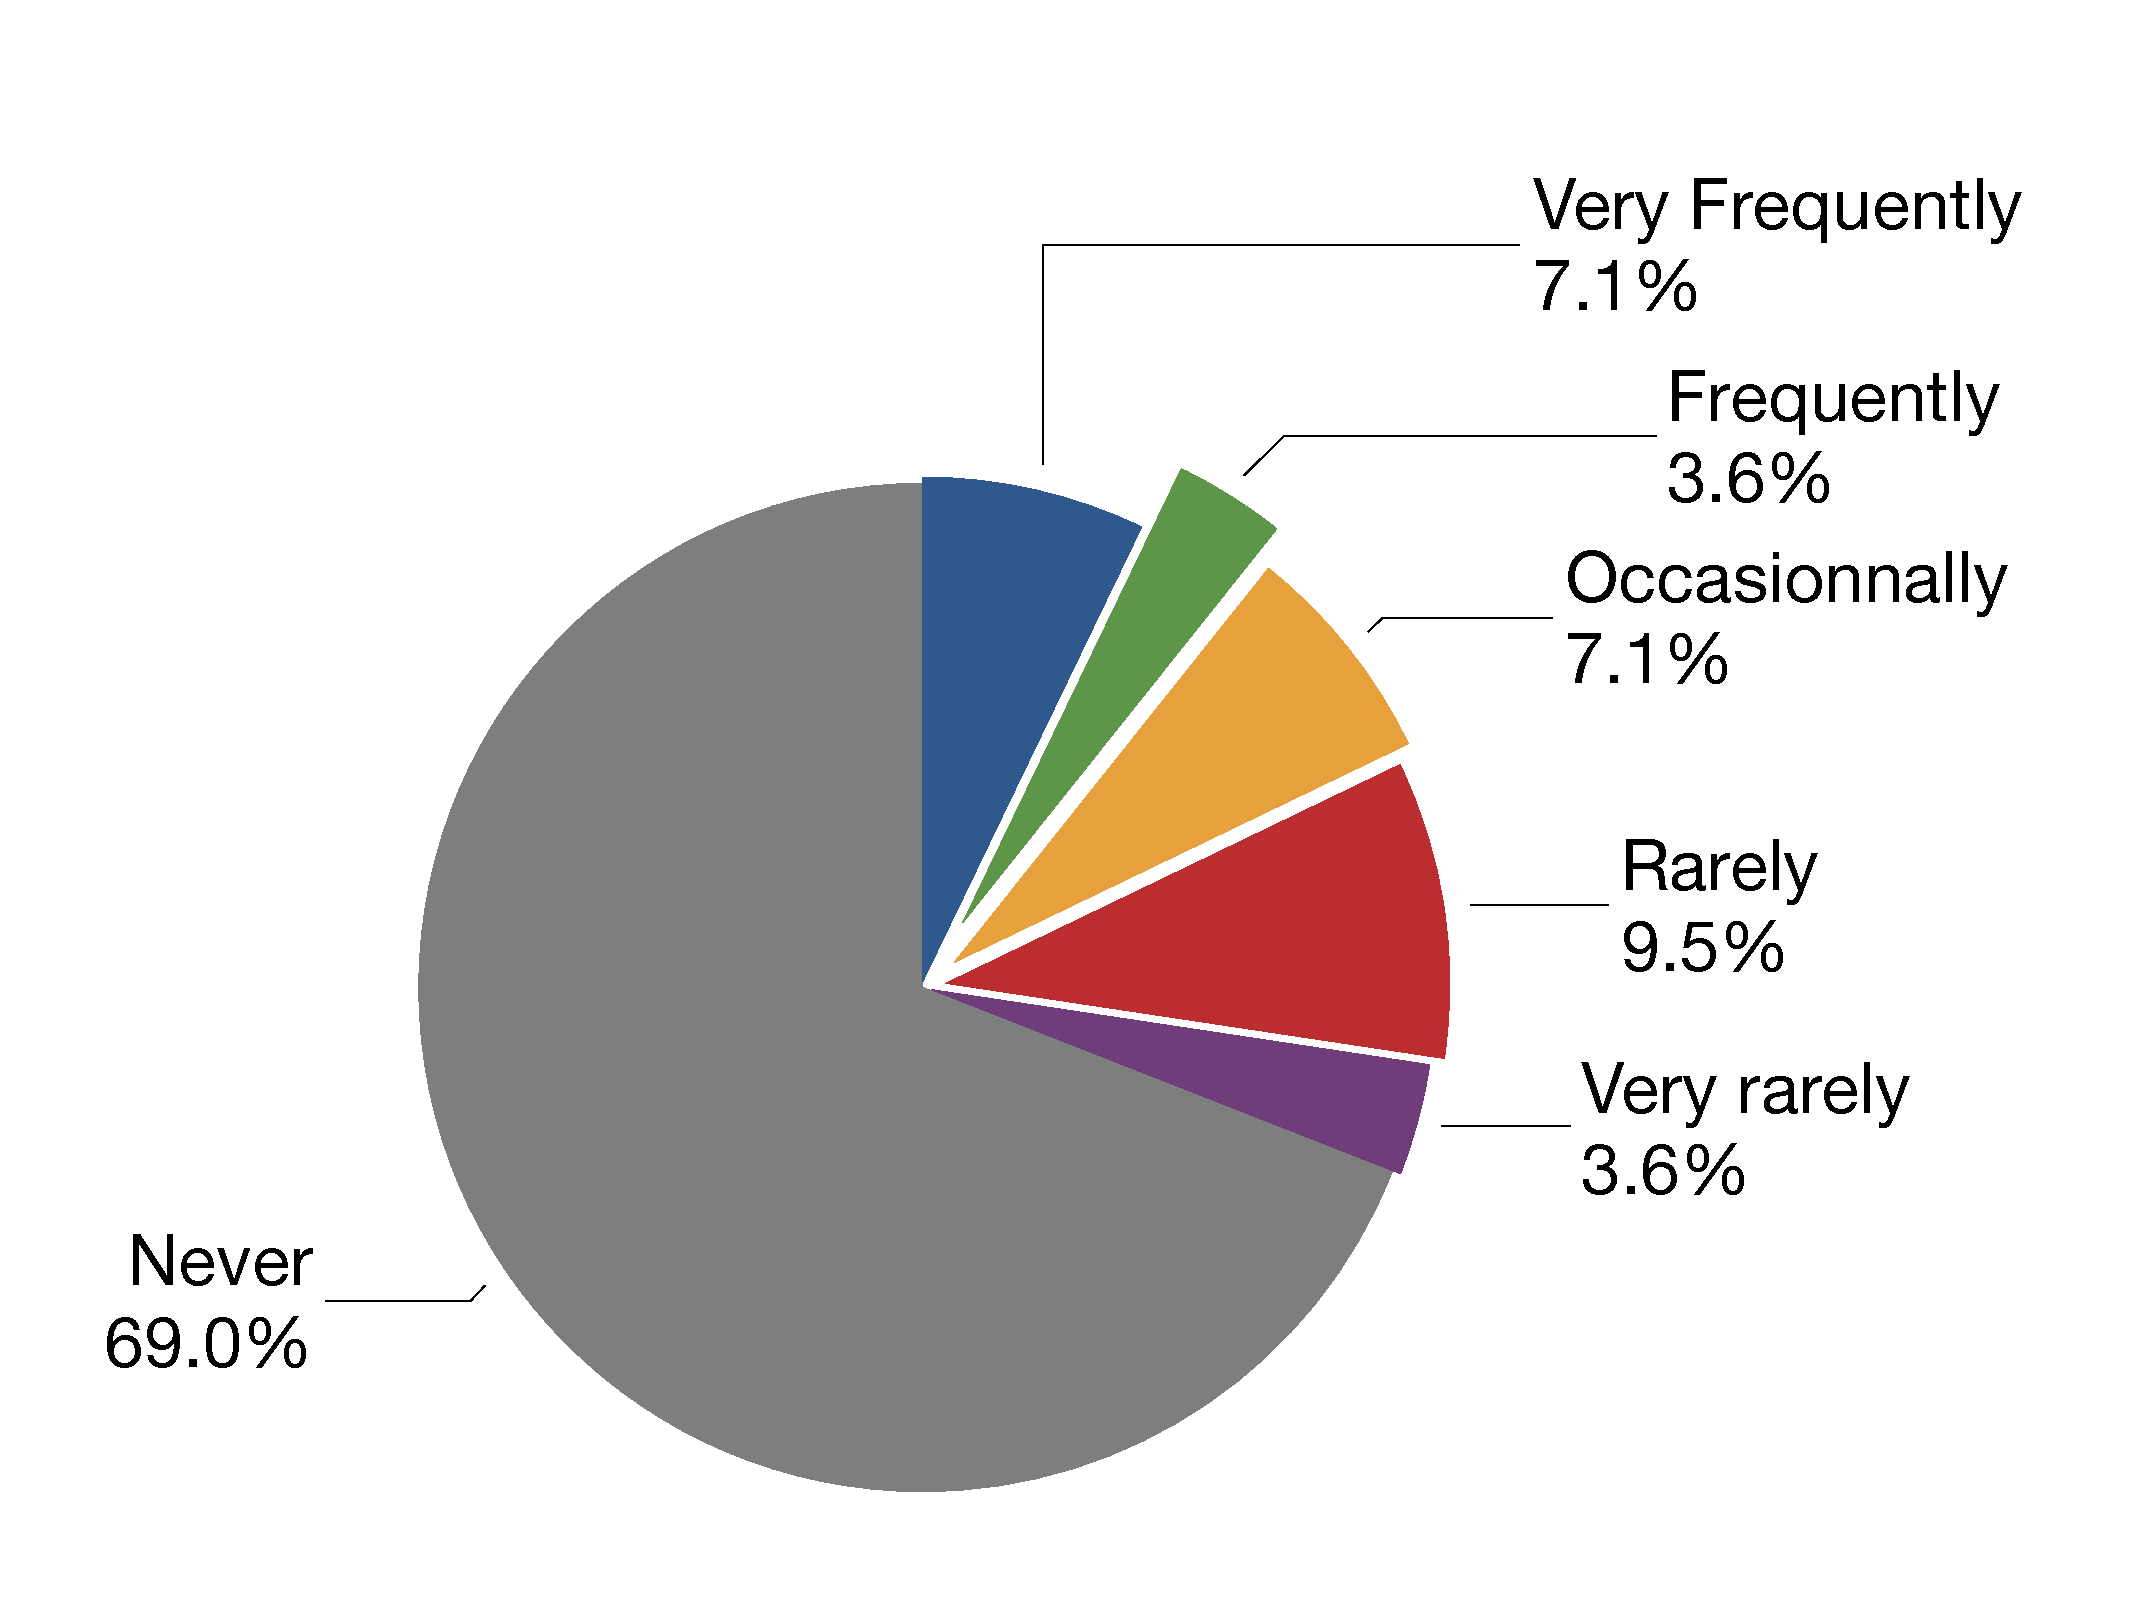
\includegraphics[width=\linewidth]{survey_license_check_2}
		\caption{Group 2}
		\label{fig:survey_license_check_2}
	\end{subfigure}
	\caption{Frequency of the answerers checking license of their code snippets against Stack Overflow's CC BY-SA 3.0.}
	\label{fig:survey_license_check}
\end{figure}

We asked the answerers a follow-up question of how frequently they checked for a conflict between software license of the code snippets they copied to their answers and Stack Overflow's CC BY-SA 3.0. As shown in \Cref{fig:survey_license_check}, approximately 69\% of answerers from both groups did not perform the checking. Nonetheless, they are about 10\% of the answerers who frequently checks for licensing conflicts when they copy code snippets to Stack Overflow.

\subsubsection{Open Comments} 
We also invited the participants to give any comments regarding answering Stack Overflow with code snippets. These are some interesting comments we received.

Comment 1: ``The real issue is less about the amount the code snippets on SO than it is about the staggeringly high number of software "professionals" that mindlessly use them without understanding what they're copying, and the only slightly less high number of would-be professionals that post snippets with built-in security issues.  A related topic is beginners who post (at times dangerously) misleading tutorials online on topics they actually know very little about. Think php/mysql tutorials written 10+ years after \texttt{mysql\_*} functions were obsolete, or the recent regex tutorial that got posted the other day on HackerNew (\url{https://news.ycombinator.com/item?id=14846506}). They're also full of toxic code snippets.''

Comment 2: ``When I copy code it's usually short enough to be considered "fair use" but I am not a lawyer or copyright expert so some guidance from SO would be helpful. I'd also like the ability to flag/review questions that violate these guidelines.''

Comment 3: ``My only concern, albeit minor, is that I know people blindly copy my code without even understanding what the code does.''

Comment 4: ``The main problem for me/us is outdated code, esp. as old answers have high google rank so that is what people see first, then try and fail. Thats why we're moving more and more of those examples to knowledge base and docs and rather link to those.''

Comment 5: ``Lot of the answers are from hobbyist so the quality is poor. Usually they are hacks or workarounds (even MY best answer on SO is a workaround).''

\subsection{Overall Discussion}
%What can we learn for the results? For example, if a developer explicitly reports in his/her code that the snippet was copied from stackoverfow, are there some benefits? We could notify - for instance - the developer when some new issues related to the snippet are posted on stackoverflow? Or could we force people posting code on SO to explicitly report licensing information? Or, could we implement an intelligent IDE that when pasting code from external resource checks for licensing violation? These of course are only some (crazy?) ideas that could be developed on the top of the results we have achieved with this study... 

%We discovered two issues regarding code snippets on Stack Overflow in this study: (1)  outdated online clones on Stack Overflow and (2) missing or incompatible license in Stack Overflow snippets. 
%that there is a considerable amount of cloned code between Stack Overflow that are cloned from 111 projects in the Qualitas corpus. 64 clone pairs are outdated and 358 snippets have incompatible software licenses to their originals. 
Our study discovers links from code in open source projects to code
snippets on Stack Overflow using clone detection techniques. These
links enable us to discover outdated code and licensing problems. The
links can be exploited further to mitigate the problems of reusing
outdated online clones and incompatible license on Stack Overflow code
snippets. We propose the following actionable items:
\begin{itemize}
	\item \textbf{Preventive measure:} We encourage Stack Overflow to enforce attribution when source code snippets have been copied ``from'' licensed software projects to Stack Overflow. Moreover, an IDE plug-in that can automatically detect pasted source code and follow the link to Stack Overflow and then to the original open source projects, could also prevent the issue of license violation.
	\item \textbf{Detective measure:} A system to detect outdated source code
	snippets on Stack Overflow is needed. The system can leverage the
	online clone detection techniques in this study to periodically check
	if the cloned snippets are still up-to-date with their
	originals. %Moreover, Stack Overflow posters have to provide the information of the project including the original file name and its online repository (if exists).
	With such a system, the poster can be notified when the code has been
	updated in the original project so that he/she can update their code
	on Stack Overflow accordingly. On the other hand, with a crowdsourcing
	solution using an IDE plug-in, developers can also report the
	corrected version of outdated code back to the original Stack Overflow
	threads when they reuse outdated code and make corrections to them.
\end{itemize}
The implementation and the evaluation of the above actionable items is part of the agenda of our future work.

\section{Threats to Validity}

\textbf{Internal validity:} 
%
We could not verify all the 315,786,118 clone pairs reported by the
clone detection tools in this study.  Nevertheless, we applied
different mechanisms to ensure the validity to the subset of clone
pairs we classified.  First, we used two widely-used
clone detection tools, Simian and NiCad.  We tried three other
clone detectors but could not add them to the study due to their
scalability issues and susceptibility to incomplete code snippets.
We mitigated the problem of clone
detector's parameter sensitivity by adding another established
configuration from the EvaClone study~\cite{Wang2013}. 
Second, we adopted Bellon's agreement metric~\cite{Bellon2007}
to prioritise and filters clone pairs for the manual
classification. The agreed clone pairs that passed \textit{good}- and
\textit{ok}- criteria had a higher chance to be true positive. 
Nevertheless, we might still suffers from false negatives, i.e.~online 
code clones that are not reported by the tools or are filtered 
out by the automatic classifier before the manual investigation.
% We also
% applied the Bellon's clone agreement to 4 different combinations of
% the tools' configurations.  For disagreed clone pairs, we applied
% several filters to remove spurious and uninteresting clones.

% The number of online clones we found are subject to the clone
% detectors and their configurations.  

% We also
% performed a pairwise matching between the default and EvaClone
% configurations of the two clone detection tools.

Our seven patterns of online code cloning may not cover all possible
online cloning patterns. However, instead of defining the patterns
beforehand, we resorted to extract them from the data sets. We derived
them from a manual investigation of 679 online clone pairs and adopted
one pattern from the study by Kapser et al.~\cite{Kapser2003}.

The 3,636 clone pairs classified by the first author are
subject to manual judgement and human errors.  Although we tried
our best to be careful on searching for evidence and classifying the
clones, some errors may still exist. We mitigated this problem by
having the second author to validate the classifications with a random
sampling. 
% The 64 classification conflicts were discussed and
% resolved.  
The third author made a final judgement when no consensus
could be found by the two authors. This validation process
can be even improved by employing an external investigator. 
%In addition, we are aware of voting mechanism
%in Stack Overflow and plan to incorporate highest-vote answers in the future work.

\textbf{External validity:} We carefully chose the data sets for our
experiment so the findings could be generalise as much as possible.
We selected Stack Overflow because it is one of the most popular
programming Q\&A websites available with approximately 6.8 million
users.  There are a large number of code snippets reused from the
site~\cite{An2017} and there are also several studies encouraging of
doing
so~(e.g.~\cite{Ponzanelli2013,Ponzanelli2014,Keivanloo2014,Park2014}).
Nonetheless, it may not be representative to all the programming Q\&A
websites.

Regarding the code snippets, we downloaded a full data dump and
extracted Java accepted answers
% Instead of analysing every post, we
%only focused on posts marked as accepted answers 
since they are the
most likely ones to be reused. 
% This yields a total of 144,064 snippets.  
Our findings are limited to these restrictions. They may
not be generalised to all programming languages and all answers on
Stack Overflow. We chose the curated Qualitas
corpus for Java open source projects containing 111 projects
\cite{QualitasCorpus}.  The projects span over several areas of
software and has been used in several empirical
studies~\cite{Taube-Schock2011,Beckman2011,Vasilescu2011,Omar2012}. Although
it is a curated and well-established corpus, it may not fully
represent all Java open source software available.

%Lastly, two clone detection tools, Simian and NiCad, are chosen for this study. We have not tried all the tools available and they might not be complete representatives of all available clone detection tools.

\section{Related Work}

\textbf{Stack Overflow} is a gold mine for software engineering
research and
% Its rich and developer-driven data are invaluable. Since
% posts on Stack Overflow may contain code snippets embedded within
% natural language text, they become a huge database for source code and
% code-relevant information. 
%The Stack Overflow data set 
has been put to
use in several previous studies. In terms of developer-assisting
tools, Seahawk is an Eclipse plug-in that searches and recommends
relevant code snippets from Stack Overflow~\cite{Ponzanelli2013}. A
follow up work, Prompter, by Ponzanelli et al.~\cite{Ponzanelli2014}
achieves the same goal but with improved algorithms. The code snippets
on Stack Overflow are mostly examples or solutions to programming
problems. Hence, several code search systems use whole or partial data
from Stack Overflow as their code search
databases~\cite{Keivanloo2014,Park2014,
	Stolee2014,Subramanian2013,Diamantopoulos2015}. Furthermore, Treude
et al.~\cite{Treude2016}~use machine learning techniques to extract
insight sentences from Stack Overflow and use them to improve API
documentation.

Another research area is knowledge extraction from Stack
Overflow. Nasehi et al.~\cite{Nasehi2012}~studied what makes a good
code example by analysing answers from Stack Overflow. Similarly, Yang
et al.~\cite{Yang2016} report the number of reusable code snippets on
Stack Overflow across various programming languages. Wang et
al.~\cite{Wang2013_StackOverflow} use Latent Dirichlet Allocation
(LDA) topic modelling to analyse questions and answers from Stack
Overflow so that they can automatically categorise new
questions. There are also studies trying to understand developers'
behaviours on Stack Overflow,
e.g.~\cite{Movshovitz-Attias2013,Rosen2016,Choetkiertikul2015,Bosu2013}.
% , while some studies aim to improve Stack Overflow itself~\cite{Diamantopoulos2015, Wang2014}. 

\textbf{Code clone detection} is a long-standing research topic in
software engineering. Whether clones are good or bad for software is
still
controversial~\cite{Sajnani2016,Kapser2003,Kapser2008,Krinke2008,Hotta2010,Gode2011,Harder2013}.
% However, by only knowing how many code clones residing in software
% and how they evolve~\cite{Pate2013,Mondal2011} can provide several
% valuable insights into the software systems.
Code clones have several
applications such as software plagiarism
detection~\cite{Prechelt2002}, source code
provenance~\cite{Davies2013}, and software licensing
conflicts~\cite{German2009}.

Two code fragments are clones if they are similar enough according to
a given definition of similarity~\cite{Bellon2007}. Given an open
interpretation of ``definition of similarity'', there are various
clone detection tools and their siblings, code plagiarism detectors,
invented based on plethora of different code similarity
measurements~\cite{Roy2008, Ragkhitwetsagul2016,Svajlenko2014}. 
% Some tools use string comparison techniques such as Simian~\cite{simian}. 
% NiCad~\cite{Roy2008,Cordy} exploits the Longest Common Subsequence
% (LCS) string similarity measure after applying code pretty-printing
% using TXL~\cite{Cordy2006}. 
Many tools do not work on original source code directly but detect clones
at an intermediate representation such as tokens ~\cite{Sajnani2016,Kamiya2002,Li2006,Gode2009,Burrows2007, Smith2009, Duric2012, Prechelt2002, Schleimer2003}, AST~\cite{Baxter1998,Jiang2007a} or program dependence
graphs~\cite{Krinke2001,Komondoor2001}. 

\textbf{Cloning patterns} is initially defined 
by Kapser et al.~\cite{Kapser2003,Kapser2008} by studying clones in 
Linux file systems and deriving 11 patterns of code cloning. 
Our study adopted one of the patterns into our online code cloning patterns.

\textbf{Clone agreement} is useful when a clone oracle is
absent. %Since clone detectors are different in their detection
%approaches, they may behave differently and report different clones
%even on the same data set. 
By exploiting the different behaviours of clone detectors,
one can look for their agreement and obtain
highly-confident clones~\cite{Bellon2007,Wang2013}. %Using the same
%data set, 
Clone pairs that are agreed by multiple tools are more assured to be true
clones than the ones reported by only a single
tool~\cite{Wang2013,cr2016ssbse,Funaro2010}. 
% There are studies that report sensitivities of the tools'
% configurations to the results~\cite{Wang2013,cr2016ssbse}, showing
% that searching for an optimal configuration for every new data set
% is preferred.

\textbf{Software licensing} is crucial for open source and 
industrial software development. Di Penta et al.~\cite{DiPenta2010}
studied the evolution of software licensing in open source 
software and found that licensing statements change over 
time. German et al.~\cite{German2009} found that licensing 
conflicts occur between the clone siblings, i.e.~clones among 
different systems that come from the same source. Later, 
German et al.~\cite{German2010} created an automated tool 
for software license identification, Ninka, which is used
in our online clone license analysis. 
%We use Ninka to analyse software license from Stack 
%Overflow snippets and Qualitas projects. 

\textbf{Reusing of outdated third-party source code} occurs 
in software development. Xia et al.~\cite{Xia2014} show that 
a large number of open source systems reuse outdated third-party 
libraries from popular open source projects. Using the outdated 
code give detrimental effects to the software since they may 
introduce vulnerabilities. Our study similarily finds
% on % the context of 
outdated code on Stack Overflow.

The work that is closely similar to us is a study by 
An et al.~\cite{An2017} where the authors investigated 
clones between 399 Android apps and Stack Overflow posts. 
They found 1,226 code snippets which were reused from 68 Android apps. 
They also observed that there are 1,279 cases of potential 
license violations. The authors rely on the timestamp to 
judge whether the code has been copied from/to Stack Overflow 
along with confirmations from six developers. Instead of Android apps, 
we investigated clones between Stack Overflow and 111 open 
source projects. Their results are similar to our findings that 
there exist clones from software projects to Stack Overflow with 
potential licensing violations. 
\FIXME{Add a discussion of Abdalkareem et al.~\cite{Abdalkareem2017}}
%In our work, we defined seven patterns of online code cloning and 
%performed a large-scale manual check of 3,632 clone pairs. 
%We discovered 112 clone pairs with strong evidences, 
%based on natural text in comments and post contents, that they 
%were copied from Qualitas to Stack Overflow. By comparing the 
%clones to their latest versions in the software, we found that 
%64 code snippets on Stack Overflow are outdated and possibly harmful for reuse.

%\section{Future Work}
%Since this study is limited to only Java language, we are interested in expanding the study further to other popular programming languages such as C, C++, Python, and Javascript on Stack Overflow. The similar study of outdated code and software licensing violation can be repeated. It is interesting to compare the findings among different programming languages. Moreover, other popular software project corpora (e.g.~GitHub) can also be included to increase generalisation of the findings.
%
%We are eager to tackle the issues of outdated and license-violating online code clones with an automated tool. The tool should incorporate a scalable clone detection method of locate similar code from programming Q\&A websites such as Stack Overflow and online code repositories like GitHub. It analyses a software project under development and reports clones that are copied from Stack Overflow. The reported clones have traces to their origins in open source projects or websites along with their freshness (fresh/outdated/dead) so that the developer of the project can be aware of changes made to the copied code snippets. Lastly, the license of the original source code is also reported so the developer can make an informed decision of whether he or she will incorporate that code snippet into their own project.

\section{Conclusions}

Online code clones are clones that have been copied to Q\&A websites
such as Stack Overflow. 
% They are similar to classical clones in software
% projects where they can be outdated and violating software license but
% are much harder to detect. 
We classified 32,533 clone pairs using seven patterns of online code
cloning.  After automatically removing boiler-plate clones, we
manually investigated 3,636 clone pairs. In the 1,216 manually
confirmed clone pairs, we discovered 112 clone pairs that have been
copied, with evidence, from Qualitas projects to Stack Overflow, 197
clone pairs that have been copied from external sources besides
Qualitas to Stack Overflow, and 359 clone pairs that are highly
similar but without evidence of copying.

We performed a detailed analysis of the online clone pairs on two
aspects: outdated code and licensing violation. The investigation of
the 112 clone pairs copied, with evidence, from Qualitas to Stack
Overflow reveals that 64 of them are outdated.  Moreover, we found 358
code snippets on Stack Overflow that violate the license of their
original software.

This study is among, if not the first, to address the important issues
of outdated and license-violating online code clones on programming
Q\&A websites using a hybrid methodology of automatic code clone
detection and a manual clone investigation.


% use section* for acknowledgment
\ifCLASSOPTIONcompsoc
  % The Computer Society usually uses the plural form
  \section*{Acknowledgments}
\else
  % regular IEEE prefers the singular form
  \section*{Acknowledgment}
\fi


The authors would like to thank...


\bibliographystyle{plain}
\bibliography{sigproc}  

% biography section
% 
% If you have an EPS/PDF photo (graphicx package needed) extra braces are
% needed around the contents of the optional argument to biography to prevent
% the LaTeX parser from getting confused when it sees the complicated
% \includegraphics command within an optional argument. (You could create
% your own custom macro containing the \includegraphics command to make things
% simpler here.)
%\begin{IEEEbiography}[{\includegraphics[width=1in,height=1.25in,clip,keepaspectratio]{mshell}}]{Michael Shell}
% or if you just want to reserve a space for a photo:

\begin{IEEEbiography}{Michael Shell}
Biography text here.
\end{IEEEbiography}

% if you will not have a photo at all:
\begin{IEEEbiographynophoto}{John Doe}
Biography text here.
\end{IEEEbiographynophoto}

% insert where needed to balance the two columns on the last page with
% biographies
%\newpage

\begin{IEEEbiographynophoto}{Jane Doe}
Biography text here.
\end{IEEEbiographynophoto}

% You can push biographies down or up by placing
% a \vfill before or after them. The appropriate
% use of \vfill depends on what kind of text is
% on the last page and whether or not the columns
% are being equalized.

%\vfill

% Can be used to pull up biographies so that the bottom of the last one
% is flush with the other column.
%\enlargethispage{-5in}



% that's all folks
\end{document}


